\documentclass[11pt,a4paper,openright,oneside]{book}
\usepackage{amsfonts, amsmath, amssymb,latexsym,amsthm, mathrsfs, enumerate}
\usepackage[utf8]{inputenc}
\usepackage[english]{babel}
\usepackage{epsfig}
\usepackage{csquotes}
\usepackage[sorting=none]{biblatex}
\usepackage{graphicx} % in real document delete demo option
\usepackage{subcaption}
\usepackage{nicematrix}
\usepackage{changepage}
\usepackage[toc]{glossaries}
\usepackage{array}

\addbibresource{refs.bib}
\addbibresource{man-refs.bib}


\parskip=5pt
\parindent=15pt
\usepackage[margin=1.2in]{geometry}
\usepackage{graphicx}
\usepackage{listings}
\usepackage{tikz}
\usepackage{tikz-cd}

\usetikzlibrary{decorations.pathreplacing}

\usepackage{parskip}
\usepackage{algorithm}
\usepackage[noend]{algpseudocode}
\usepackage{hyperref}
\usepackage{cleveref}
\usepackage{color}
\hypersetup{
    linktoc=all,
    % linkcolor=blue,  %choose some color if you want links to stand out
}

\setcounter{page}{0}



\numberwithin{equation}{section}
\newtheorem{defn0}{Definition}[chapter]
\newtheorem{prop0}[defn0]{Proposition}
\newtheorem{thm0}[defn0]{Theorem}
\newtheorem{lemma0}[defn0]{Lemma}
\newtheorem{corollary0}[defn0]{Corollary}
\newtheorem{example0}[defn0]{Example}
\newtheorem{remark0}[defn0]{Remark}
\newtheorem{conjecture0}[defn0]{Conjecture}

\newenvironment{definition}{ \begin{defn0}}{\end{defn0}}
\newenvironment{proposition}{\bigskip \begin{prop0}}{\end{prop0}}
\newenvironment{theorem}{\bigskip \begin{thm0}}{\end{thm0}}
\newenvironment{lemma}{\bigskip \begin{lemma0}}{\end{lemma0}}
\newenvironment{corollary}{\bigskip \begin{corollary0}}{\end{corollary0}}
\newenvironment{example}{ \begin{example0}\rm}{\end{example0}}
\newenvironment{remark}{ \begin{remark0}\rm}{\end{remark0}}
\newenvironment{conjecture}{\begin{conjecture0}}{\end{conjecture0}}

\newcommand{\defref}[1]{Definition~\ref{#1}}
\newcommand{\propref}[1]{Proposition~\ref{#1}}
\newcommand{\thmref}[1]{Theorem~\ref{#1}}
\newcommand{\lemref}[1]{Lemma~\ref{#1}}
\newcommand{\corref}[1]{Corollary~\ref{#1}}
\newcommand{\exref}[1]{Example~\ref{#1}}
\newcommand{\secref}[1]{Section~\ref{#1}}
\newcommand{\remref}[1]{Remark~\ref{#1}}
\newcommand{\conjref}[1]{Conjecture~\ref{#1}}
\newcommand{\figref}[1]{\cref{#1}}
\newcommand{\refeq}[1]{\cref{#1}}



\DeclareMathOperator{\vectorize}{vec}
\DeclareMathOperator{\rank}{rank}
\DeclareMathOperator{\unfolding}{unfold}
\DeclareMathOperator{\folding}{fold}
\DeclareMathOperator{\reshape}{reshape}
\DeclareMathOperator{\IN}{IN}
\DeclareMathOperator{\OUT}{OUT}
\DeclareMathOperator{\TNS}{TNS}
\DeclareMathOperator*{\argmax}{arg\,max}
\DeclareMathOperator*{\argmin}{arg\,min}
\DeclareMathOperator{\Tr}{Tr}
\DeclareMathOperator{\size}{Size}
\DeclareMathOperator{\Det}{Det}
\DeclareMathOperator{\Diag}{Diag}

% --------------------------------------------------
\usepackage{fancyhdr}

\lhead{}
\lfoot{}
\rhead{}
\cfoot{}
\rfoot{\thepage}

\makeglossaries
% Glossary
\newglossaryentry{TN}
{
    name=TN,
    description={Tensor Network}
}

\newglossaryentry{TnALE}
{
    name=TnALE,
    description={Tensor network Alternating Local Enumeration algorithm}
}

\newglossaryentry{TnALS}
{
    name=TnALS,
    description={Tensor network Alternating Least Squares algorithm}
}

\newglossaryentry{TNS}
{
    name=TNS,
    description={Tensor Network States}
}

\newglossaryentry{LSQ}
{
    name=LSQ,
    description={Least Squares problem}
}

\newglossaryentry{SVD}
{
    name=SVD,
    description={Singular Value Decomposition}
}
\newglossaryentry{TN-RS}
{
    name=TN-RS,
    description={Tensor Network Rank Selection problem}
}
\newglossaryentry{TN-PS}
{
    name=TN-PS,
    description={Tensor Network Permutation Selection problem}
}
\newglossaryentry{TN-TS}
{
    name=TN-TS,
    description={Tensor Network Topology Selection problem}
}
\newglossaryentry{FCNN}
{
    name=FCNN,
    description={Fully Connected Neural Network}
}
\newglossaryentry{TR}
{
    name=TR,
    description={Tensor Ring}
}
\newglossaryentry{TT}
{
    name=TT,
    description={Tensor Train}
}
\newglossaryentry{MPS}
{
    name=MPS,
    description={Matrix Product State}
}
\newglossaryentry{FCTN}
{
    name=FCTN,
    description={Fully Connected Tensor Network}
}
\newglossaryentry{CR}
{
    name=CR,
    description={Compression Rate}
}

\begin{document}

\bibstyle{plain}



\thispagestyle{empty}

\begin{titlepage}
\begin{center}
\begin{figure}[htb]
\begin{center}

\includegraphics[width=6cm]{matematiquesinformatica-pos-rgb.png}
\end{center}
\end{figure}

\vspace*{1cm}
\textbf{\LARGE GRAU DE MATEM\`{A}TIQUES } \\
\vspace*{.5cm}
\textbf{\LARGE Treball final de grau} \\

\vspace*{1.5cm}
\rule{16cm}{0.1mm}\\
\begin{Huge}
\textbf{SEARCH OF OPTIMAL LOW-RANK APPROXIMATIONS USING TENSOR NETWORKS} \\
\end{Huge}
\rule{16cm}{0.1mm}\\

\vspace{1cm}

\begin{flushright}
\textbf{\LARGE Autor: Aran Roig}

\vspace*{2cm}

\renewcommand{\arraystretch}{1.5}
\begin{tabular}{ll}
\textbf{\Large Director:} & \textbf{\Large Dr. Nahuel Norberto Statuto Perez} \\
\textbf{\Large Realitzat a:} & \textbf{\Large  Departament de Matemàtiques   } \\
 & \textbf{\Large i Informàtica} \\
\\
\textbf{\Large Barcelona,} & \textbf{\Large \today }
\end{tabular}

\end{flushright}

\end{center}



\end{titlepage}


\newpage
\pagenumbering{roman} 

\section*{Abstract}

Tensor network structure search has been interesting research topic since the raise on
complexity of deep learning models and quantum mechanics. This Bachelor Thesis main goal is to give an 
automated search of an optimal tensor network structure that gives the best low-rank approximation of a given 
tensor.

For these purpose we first give an introduction to some basic tensor algebra, we present tensor networks and tensor
network states. Then we present algorithms that find the cores of a tensor network that better represent an objective tensor.
We also present an algorithm for finding optimal tensor network structures that can guarantee that we will find
the most optimal cores.

Finally, we prove that these algorithms converge under certain assumptions and then we perform
some practical experiments that empirically proves that it is possible to find other more optimized low-rank decompositions of tensors
without significant losses on performance and accuracy.

\section*{Resum}

La recerca de l'estructura òptima de xarxes de tensors ha estat un tema d'interès des de l'augment en la complexitat dels models d'aprenentatge profund i de la mecànica quàntica. 
Aquest treball de final de grau té com a objectiu principal oferir una cerca automatitzada 
d’una estructura òptima d'una xarxa de tensors que representi millor un tensor amb una aproximació de baix rank.

Per aconseguir aquest propòsit, primer oferim una introducció als tensors, a les xarxes tensorials. 
Aleshores presentem algoritmes que troben els nuclis de la xarxa tensorial que millor representen un tensor objectiu.
També presentem un algoritme per trobar quina estructura de xarxa tensorial ens pot garantir que poguem trobar els nuclis més optims.

Finalment demostrem que aquests algoritmes convergeixen sota algunes suposicions i després fem
uns quants experiments que empíricament mostren que és possible trobar altres descomposicions de baix rang de tensors
sense que suposin una pèrdua significant en rendiment i precissió.

% TODO: Omplir això
% 15A69 - Multilinear Algebra, Tensor Calculus, Graph Theory, no se
{\let\thefootnote\relax\footnote{2020 Mathematics Subject Classification. 11G05, 11G10, 14G10}}



\newpage 


\section*{Agra\"{\i}ments}

Vull agrair a ... 
\newpage

{\hypersetup{linkcolor=black}
\tableofcontents
}

\newpage
\printglossary[title=Glossary]
\newpage
\pagenumbering{arabic} 
\setcounter{page}{1}
\chapter{Introduction}


% TODO: Fer mes intro a les nn, com afecten al món, i tal.
Over the last years, high-dimensional data has become ubiquitous in modern science and engineering,
arising in areas such as quantum many-body physics and machine learning. However, as the dimensionality of the
data increases, so does the burden of the increase of computational and storage cost often referred
as the curse of dimensionality. To address this challenge, low-rank approximation techniques have emerged as powerful tools,
enabling the efficient representation, compression, and manipulation of large-scale tensors. Recent research 
has proven promising results in the capabilities of compression of
tensor networks. Qing et. al. for example see empirically that tensor networks can be very useful
for neural network parameter compression \cite{qingCompressingNeuralNetworks2025} or even image
recovering \cite{lyuMultiDimensionalImageRecovery2022}

Sometimes, the low-rank approximation of a given tensor is not guaranteed to be represented from
a fixed tensor network structure. There has been a lot of recent research on solving
the problem on finding the optimal structures. On \cite{liPermutationSearchTensor2022} Li et. al. 
present an algorithm that aims to find an optimal tensor network permutation.
We will see in more detail the Tensor network Alternating Local Enumeration (\gls{TnALE}) algorithm presented
by Li. et. al on \cite{liAlternatingLocalEnumeration2023}. The presented algorithm aims to
solve the rank search of the core tensors and the optimal permutation. We will extend this algorithm
for also solving the structure search of tensor networks.

The concept of tensor networks appeared from the study of many-body quantum systems \cite{orusTensorNetworksComplex2019}
and recently has attracted significant interest on machine learning. 
Foundamental research on tensor networks started
in $1971$ by the paper "Applications of negative dimensional tensors". In which
he introduced the Penrose Notation for representing contractions of various tensors, and how this
diagrammatic approach could be used in various applications in physics \cite{biamonteLecturesQuantumTensor2020}. Forwarding
to recent years, on 2014, Román Orus \cite{181204011TensorNetworks} and later in 2019 presented the first
idea of applying them in machine learning \cite{orusTensorNetworksComplex2019}.

The main goal of this thesis will be to compress tensors by getting a low-rank approximation of them by
finding an approximate representation of a given tensor network state. We will present two different algorithms
for achieving this goal: the Tensor network Alternating Least Squares (\gls{TnALS}) algorithm and backpropagation. We will compare these two algorithm and we will
discuss their use cases. Then, we will present the \gld{TnALE} algorihtm and we will prove its convergence
presenting beforehand zero gradient theory.

Finally, we will do some experiments with these algorithms: we will perform lossy compression on images and
also we will compress the parameters of a simple neural network.

%\section{Objectives}

\section{Thesis structure}

% TODO: Cambiar això una mica

The second chapter of the thesis will focus on the preliminaries about tensor algebra. We will introduce 
tensors from a mathematical standpoint presenting the tensor product space.
We will see that the tensor product space forms vector space and then we will describe
some operations between tensors.

After that, we will also describe some reshaping operations that can be applied to tensors to transform its
orders i.e their number of dimensions. These reshaping operations will be useful on the following chapters
since we will need them for presenting the TnALS algorithm and also for the last chapter of applications, when
we transform matrices into tensors and then apply all the theory that we have presented.

On the third chapter we will present the basics of the Penrose Notation and we will give a formal
definition to tensor networks and tensor network states (\gls{TNS}). We will give some
common examples of tensor networks and after that we will define the notion
of the rank of a tensor related to a TNS, called $G$-rank. We will see that the $G$-rank can be a lot smaller
than the traditional tensor rank as it is discussed in \cite{yeTensorNetworkRanks2019},
proving that there exists better compression methods than the canonical
polyadic decomposition, which we will see on the same chapter.

On the fourth chapter we will describe the main algorithms of this thesis. First, we will give two algorithms
that fixed a tensor network (\gls{TN}), finds a low-rank decomposition of smaller tensors that can represent our original tensor
with a certain error. These algorithms are the \gls{TnALS} and the backpropagation algorithm.
We will also solve this problem using backpropagation.

Then, we will unfix the tensor structure and we will present the \gls{TnALE} algorithm which finds the most optimal
tensor network structure for representing a tensor $T$ by evaluating a loss function that depends on the
structure itself. The advantage of TnALE respect other algorithms
is that it also saves some evaluations of some tensor network structure candidates. Lastly we will prove
that \gls{TnALE} converges to an optimal structure, and also we will prove the fact of
skipping certain evaluations, all of this under some given assumptions.

Finally on the fifth chapter we will apply all of these algorithms for practical cases such as compressing images,
compressing the weight matrices of fully connected neural networks.

\chapter{Tensors}


\iffalse
\begin{definition}[Graph isomorphisms]
    We say that two graphs $G, H$ are \textbf{isomorphic} if 
\end{definition}


\begin{definition}[Outer product]
    We define the \textbf{outer product} of $n$ vectors 
    $a_1 \in \mathbb{R}^{N_1}, a_2 \in \mathbb{R}^{N_2}, \dots, a_n \in \mathbb{R}^{N_n}$
    as the $n$th-order tensor $\mathcal{T} \in \mathbb{R}^{N_1 \times N_2 \times \dots \times N_n}$ with its entries being
    $$\mathcal{T}(i_1, \dots, i_n) = a_1(i_1) a_2(i_2) \cdots a_n(i_n)$$
\end{definition}

\begin{example}
The outer product of two vectors $a \in \mathbb{R}^I$ and $b \in \mathbb{R}^J$ is denoted by $a \circ b$ and it results
as a matrix $M = a \circ b \in \mathbb{R}^{I \times J}$ with its entries defined as $M_{ij} = a_i b_j$.
\end{example}


\begin{definition}[Inner product]
The inner product of two tensors $\mathcal{X}, \mathcal{Y} \in \mathbb{R}^{N_1 \times \cdots \times N_n}$ is defined by
$$\langle \mathcal{X},\mathcal{Y} \rangle = \sum_{i_1, \dots, i_N}^{N_1, \dots, N_n} \mathcal{X}_{i_1, \dots, i_n} \mathcal{Y}_{i_1, \dots, i_n} = 
\vectorize(\mathcal{X})^T \vectorize(\mathcal{Y}) = \langle \vectorize(\mathcal{X}), \vectorize(\mathcal{Y}) \rangle$$
\end{definition}


\begin{definition}[Kronecker product]
    \normalfont{\cite{panagakisTensorMethodsComputer2021}} Given two matrices $A \in \mathbb{R}^{N_1 \times N_2}$ and $B \in \mathbb{R}^{M_1 \times M_2}$,
    their kronecker product is defined as the matrix $A \otimes B \in \mathbb{R}^{N_1 \cdot M_1 \times N_2 \cdot M_2}$ with
    $$A \otimes B = \begin{bmatrix}
        a_{11}B & \cdots & a_{1N_2}B \\ 
        \vdots & \ddots & \vdots \\
        a_{N_1 1}B & \cdots & a_{N_1 N_2}B \\
    \end{bmatrix}$$
\end{definition}

\begin{definition}[Khatri-Rao product]
    \normalfont{\cite{panagakisTensorMethodsComputer2021}} Given two matrices $A \in \mathbb{R}^{N \times R}$ and $B \in \mathbb{R}^{M \times R}$ their
Khatri-Rao, also known as column-wise Kronecker product is defined as $A \odot B \in \mathbb{R}^{N \cdot M \times R}$
    $$ A \odot B = \begin{bmatrix} A_{:,1} \otimes B_{:,1} & A_{:,2} \otimes B_{:,2} & \cdots & A_{:,R} \otimes B_{:,R}  \end{bmatrix}$$
        

\end{definition}

\begin{definition}[Frobenius norm]
The \textbf{Frobenius norm} of a tensor $\mathcal{T} \in \mathbb{R}^{N_1 \times \cdots \times N_n}$ is given by
$$\|\mathcal{T}\|_F = \sqrt{\langle \mathcal{T}, \mathcal{T} \rangle} = \sqrt{\sum_{i_1, \dots, i_n}^{N_1, \dots, N_n}
\mathcal{T}_{i_1 \dots i_n}^2}$$
\end{definition}

\begin{definition}[Tensor transposition]
    \normalfont{\cite{zhengFullyConnectedTensorNetwork2021}} Let $\mathcal{T} \in \mathbb{R}^{N_1 \times \cdots \times N_n}$
    be an $n$th-order tensor and $p$ a permutation of the vector $(1, 2, \dots, n)$. We define the \textbf{vector $p$ based tensor
    transposition of $\mathcal{T}$} as the tensor $\overrightarrow{\mathcal{T}_p} \in \mathbb{R}^{N_{p_1} \times \cdots \times N_{p_n}}$ with its entries defined as follows:
    $$\overrightarrow{\mathcal{T}_p}(i_1, i_2, \cdots, i_n) = (i_{p_1}, i_{p_2}, \cdots, i_{p_n})$$
\end{definition}

\begin{definition}[Tensor contraction]
    \normalfont{\cite{zhengFullyConnectedTensorNetwork2021}} Suppose that $p$ and $q$ are reorderings of the vectors
    $(1,2,\dots,n)$ and $(1,2,\dots,m)$ respectively, and let ${\mathcal{X} \in \mathbb{R}^{N_1 \times \cdots \times N_n}}$ 
    and $\mathcal{Y} \in \mathbb{R}^{M_1 \times \cdots \times M_m}$ two tensors with $N_{p_i} = M_{q_i}$ for all $i = 1,2,\dots,d$
    with $d \leqslant \min{(n, m)}$. We define the tensor contraction along the $p_{1:d}$-modes of $\mathcal{X}$ and the $q_{1:d}$-modes
    of $\mathcal{Y}$ as the tensor $\mathcal{Z}$ of order $n + m - 2d$
$$\mathcal{Z} = \mathcal{X} \times_{p_{1:d}}^{q_{1:d}} \mathcal{Y} \in \mathbb{R}^{N_{p_{d+1}} \times \cdots \times N_{p_{n}} \times N_{q_{d+1}} \times \cdots \times N_{q_m}}$$
whose elements are defined by:
$$\mathcal{Z}(i_{p_{d+1}}, \cdots, i_{p_n}, j_{q_{d+1}}, \cdots, j_{q_m}) = $$$$ \sum_{i_{p_1} = 1}^{N_1} \sum_{i_{p_2} = 1}^{N_2} \cdots \sum_{i_{p_d} = 1}^{N_d}
\overrightarrow{\mathcal{X}_p}(i_{p_1}, \cdots, i_{p_d}, i_{p_{d+1}}, \cdots, i_{p_n}) \overrightarrow{\mathcal{Y}_q}(i_{p_1}, \cdots, i_{p_d}, j_{q_{d+1}}, \cdots, j_{q_m})$$
\end{definition}



\fi


In this chapter we will construct tensors in a formal way and we will lay down the basics of tensor algebra. We will
define the notion of rank of a tensor and then,
we will describe some basic tensor reshaping operations.
All of this will be crucial for then presenting tensor contractions and \gls{TN}s on the following chapter.

\section{The tensor product space}

From now on, we will denote $\mathbb{V}_1, \dots, \mathbb{V}_n$ as finite vector spaces over a field $\mathbb{K}$ ($\mathbb{R}$ if unspecified) of dimension $\dim{\mathbb{V}_i} = N_i \; \forall i = 1, \dots, n$.

We will now present the definition of a tensor. One of the most simple definitions for presenting a tensor
are multilinear maps:

\begin{definition}
    A \textbf{multilinear map} is a mapping ${T: \mathbb{V}_1 \times \dots \times \mathbb{V}_n \rightarrow \mathbb{K}}$ which satisfies:
    \begin{enumerate}
        \item $T(v_1, \dots, \lambda v_i, \dots, v_n) = \lambda \cdot T(v_1, \dots, v_i, \dots, v_n)$
        \item $T(v_1, \dots, v_i + u, \dots, v_n) = T(v_1, \dots, v_i, \dots, v_n) + T(v_1, \dots, u, \dots, v_n) \\ {\forall i = 1, \dots, n, \; u \in \mathbb{V}_i, \lambda \in \mathbb{K}}$
    \end{enumerate}
    \label{def:multilinear-maps}
\end{definition}


We will call multilinear maps tensors. The order of a tensor will be defined as the value of $n$.
For example, kinear maps and bilinear maps are specific cases of tensors with $n=1$ and $n=2$ respectively.

This definition gives a clear intuition about what is a tensor, but it doesn't extract all of the properties that tensor have.
For example, following this definition it is not obvious that all multilinear maps $T: \mathbb{V}_1 \times \cdots \mathbb{V}_n \rightarrow \mathbb{K}$
form a vector space. The next thing that we are going is transform this definition so that we can define tensors
as an element of a given vector space. We will achieve this define by defining a relation between all the vectors in the free vector space
over the cartesian product of $\mathbb{V}_1 \times \cdots \times \mathbb{V}_n$ that capture the properties of multilinear maps.

The first ingredient that we will need is defining what are the free vector spaces over a set:

\begin{definition} Let $S$ be a set and $\mathbb{K}$ a field. We denote the free vector space over $S$ as $\mathbb{K}[S]$, which
    is the vector space containing all linear combinations of elements from $S$ with coefficients of $\mathbb{K}$, i.e:
    $$\mathbb{K}[S] = \left\{ \sum_{i=1}^n a_i s_i \mid s_i \in S, n \in \mathbb{Z}_+, a_i \in \mathbb{K}  \right\}$$
\end{definition}

\begin{example} If we take $\mathbb{K} = \mathbb{R}$ and $S = (x,y)$, then the elements of $\mathbb{R}[S]$ have the form $ax + by$ with $a, b \in \mathbb{R}$.
We can clearly see  that $\mathbb{R}[S]$ is a vector space of dimension $2$ over the field $\mathbb{R}$ and therefore
isomorphic to $\mathbb{R}^2$
\end{example}

Now we will present the relation of each element of the free vector space of $\mathbb{V}_1 \times \cdots \times \mathbb{V}_n$ and
multilinear maps.

Let $\mathbb{L} = \mathbb{K}[\mathbb{V}_1 \times \dots \times \mathbb{V}_n]$.
    We define relation $\sim_R$ as the smallest equivalence relation that satisfies: 
    $$(v_1, \dots, \alpha v_i, \dots, v_n) \sim_R \alpha(v_1, \dots, v_n) \; \forall i = 1, \dots, n, \forall \alpha \in \mathbb{K}$$
    $$(v_1, \dots, v_i + u_i, \dots, v_n) \sim_R (v_1, \dots, v_i \dots, v_n) + (v_1, \dots, u_i, \dots, v_n) \; \forall i = 1, \dots, n$$

\begin{proposition}
    $[0]_R$ is a subspace of $\mathbb{K} \left[ \mathbb{V}_1 \times \cdots \mathbb{V}_n \right]$

    \begin{proof}
        $0 \in [0]_R$. It is sufficient to see that for all $\lambda \in \mathbb{K}$ and $u, v \in [0]_R$ then $u + \lambda v \in [0]_R$.
        We can write $u + \lambda v \sim_R (u_1 + v_1, \dots, u_i + \lambda v_i, \dots, u_n + v_n) \sim_R 
        (u_1, \dots, u_n) + (v_1, \dots, \lambda v_i, \dots, v_n) \sim_R 0 + \lambda 0 \sim_R 0$ and therefore
        $u + \lambda v \sim_R 0$ since $R$ is an equivalence relation.
    \end{proof}
\end{proposition}

Because of this proposition, the quotient space $\mathbb{L} / [0]_R$ is well defined.

\begin{definition} 
    The \textbf{tensor product space} $\mathbb{V}_1 \otimes \dots \otimes \mathbb{V}_n$ is defined as the quotient $\mathbb{L} / [0]_R$. 
    Each element of the tensor product space is the image of the quotient mapping ${\varphi: \mathbb{L} \rightarrow \mathbb{L} / [0]_R}$
    defined by sending each element $(v_1, \dots, v_n) \in \mathbb{L}$ to its equivalence class that we
    will write as $v_1 \otimes \dots \otimes v_n$. 
\end{definition}

We will give an small example of a tensor product space:

\begin{example}
    Given $\mathbb{R}^2$ and $\mathbb{R}^3$ with its canoncial vector space
    structures, $\mathbb{R}^2 \otimes \mathbb{R}^3$ is defined by the equivalence classes that follow the relations
    $$(\alpha u, v) \sim \alpha (u, v) \sim (u, \alpha v) \quad \forall \alpha \in \mathbb{K}, \; u \in \mathbb{R}^2, v \in \mathbb{R}^3$$
    $$(u + u', v) \sim (u, v) + (u' + v) \quad \forall u, u' \in \mathbb{R}^2, v \in \mathbb{R}^3$$
    $$(u, v + v') \sim (u, v) + (u + v') \quad \forall u \in \mathbb{R}^2, v, v' \in \mathbb{R}^3$$
    And an element of $\mathbb{R}^2 \otimes \mathbb{R}^3$ would be the representant of $[((1, 2, 3), (0, 4))]$ in which
    for example other representants of the same equivalence class would be $2 \cdot ((1,2,3), (0, 2))$ or ${((1, 0, 3), (0, 2)) + ((0,2,0), (0, 2))}$
\end{example}
% \begin{definition}[Order of a tensor] Given a tensor $T \in \mathbb{V}_1 \times \cdots \times \mathbb{V}_n \rightarrow \mathbb{K}$ We define the \textbf{order} of the tensor $T$ as $n$.
% \end{definition}


We will now state and prove the universal property of the tensor product:

\begin{theorem}[Universal property of the tensor product]
    Let $\varphi$ be the quotient mapping from $\mathbb{V}_1 \times \cdots \times \mathbb{V}_n$ to $\mathbb{V}_1 \otimes \cdots \otimes \mathbb{V}_n$. 
    For every multilinear map $h: \mathbb{V}_1 \times \cdots \times \mathbb{V}_n \rightarrow X$ where $X$ is any vector space there exists an unique linear map 
    $\tilde{h}: \mathbb{V}_1 \otimes \cdots \otimes \mathbb{V}_n \rightarrow X$ such that the following diagram commutes:

    \centering
% https://q.uiver.app/#q=WzAsMyxbMCwwLCJWXFx0aW1lcyBXIl0sWzEsMCwiViBcXG90aW1lcyBXIl0sWzEsMSwiWCJdLFswLDEsIlxcdmFycGhpIl0sWzAsMiwiaCIsMl0sWzEsMiwiXFx0aWxkZSBoIl1d
\begin{tikzcd}
	{\mathbb{V}_1 \times \cdots \times \mathbb{V}_1} & {\mathbb{V}_1 \otimes \cdots \otimes \mathbb{V}_n} \\
	& X
	\arrow["\varphi", from=1-1, to=1-2]
	\arrow["h"', from=1-1, to=2-2]
	\arrow["{\tilde h}", from=1-2, to=2-2]
\end{tikzcd}


\begin{proof}
    Let $\varphi(v_1, \dots, v_n) := [(v_1, \dots, v_n)] \in \mathbb{V}_1 \otimes \cdots \otimes \mathbb{V}_n$. Let $h : \mathbb{V}_1 \times \cdots \mathbb{V}_n \rightarrow X$ be a
    multilinear map. We define $\tilde H : \mathbb{K}[\mathbb{V}_1 \times \cdots \times \mathbb{V}_n] \rightarrow X$ by:
    $$\tilde H \left( \sum_{i=1}^p a_i (v_i^1, \dots, v_i^n) \right) := \sum_{i=1}^p a_i h(v_i^1, \dots, v_i^n) $$
    Consider now the vector subspace $[0]_R$ of $\mathbb{K}[\mathbb{V}_1 \times \cdots \times \mathbb{V}_n]$.
    Since $h$ is multilinear, we can see that $\tilde H$ sends every element of $[0]_R$ to
    $0 \in X$, therefore $W \subseteq \ker{ \tilde H}$ and hence $\tilde H$ induces a well-defined linear map $\tilde h: \mathbb{K}[\mathbb{V}_1 \times \cdots \times \mathbb{V}_n]/R = \mathbb{V}_1 \otimes \cdots \otimes \mathbb{V}_n \rightarrow X$
    that satisfies $\tilde h (v_1 \otimes \cdots \otimes v_n) = h(v_1, \dots, v_n)$

    Suppose that exists another mapping $f : \mathbb{V}_1 \otimes \cdots \otimes \mathbb{V}_n \rightarrow X$ such that $f(v_1 \otimes \cdots \otimes v_n) = h(v_1, \dots, v_n)$, then we would have
    $$f \left( \sum_{i=1}^p a_i v_i^1 \otimes \cdots \otimes v_i^n \right) = \sum_{i=1}^p a_i h(v_i^1, \dots, v_i^n) = \tilde h \left( \sum_{i=1}^n a_i v_i^1 \otimes \cdots \otimes v_i^n \right)$$
    therefore, the linear mapping $\tilde h$ is unique
\end{proof}
\end{theorem}

An interesting observation of the universal property of tensor products is that if we take any multilinear map ${T: \mathbb{V}_1 \times \cdots \times \mathbb{V}_n \rightarrow X}$
and we fix $X$ to be the field $\mathbb{K}$, then there exists an unique linear map $\tilde T: \mathbb{V}_1 \otimes \cdots \otimes \mathbb{V}_n \rightarrow \mathbb{K}$
which is an element of the dual space $(\mathbb{V}_1 \otimes \cdots \otimes \mathbb{V}_n)^*$ which is isomorphic to $\mathbb{V}_1 \otimes \cdots \otimes \mathbb{V}_n$, proving
that the multilinear maps that we have defined at \defref{def:multilinear-maps} are isomorphic to the elements of the tensor product space
$\mathbb{V}_1 \otimes \cdots \otimes \mathbb{V}_n$



% TODO: Posar on es demostra això o demostrar-ho
\iffalse
The universal property of the tensor product can be extended to the tensor product of more than two spaces by changing the condition
of bilinearity to multilinearity: If we consider the tensor product $\mathbb{V}_1 \otimes \cdots \otimes \mathbb{V}_n$, for every
multilinear map $h : \mathbb{V}_1 \times \cdots \times \mathbb{V}_n \rightarrow X$ then there exists an unique linear map
$\tilde h : \mathbb{V}_1 \otimes \cdots \otimes \mathbb{V}_n \rightarrow X$ with $h = \varphi \circ \tilde h$
\fi

Also, thanks to this theorem we explicitly construct the vector space ${\mathbb{V}_1 \otimes \dots \otimes \mathbb{V}_n}$ and a
basis of it:

\begin{proposition} Let $\{e_1^i, e_2^i, \dots, e_{N_i}^i\}$ be basis for each $\mathbb{V}_i$ and $N_i = \dim \mathbb{V}_i$. Then the set
$$\mathcal{B}_{\otimes} = \{e_{i_1}^1 \otimes \cdots \otimes e_{i_n}^n = [(e_{i_1}^1, \dots, e_{i_n}^n)]_R : 1 \leqslant i_j \leqslant N_j, 1 \leqslant j \leqslant n\}$$
is a basis of $\mathbb{V}_1 \otimes \cdots \otimes \mathbb{V}_n$.
\begin{proof}
If we have $v_1 \otimes \cdots \otimes v_n \in \mathbb{V}_1 \otimes \cdots \otimes \mathbb{V}_n$, if we write
$v_i = \displaystyle\sum_{j=1}^{N_i} \lambda_j^i e_j^i$ then, because of the multilinearity of $R$ we get that
$$v_1 \otimes \cdots \otimes v_n = \left(\sum_{i=1}^{N_1} \lambda_1^i e_1^i \right) \otimes \cdots \otimes 
\left( \sum_{i=1}^{N_n} \lambda_n^i e_n^i \right) = \sum_{s_1, \dots, s_n}^{N_1, \dots, N_n} \lambda_{1}^{s_1} \cdots \lambda_n^{s_n} (e_1^{s_1} \otimes \cdots \otimes e_n^{s_n})$$
And since all elements of $\mathbb{V}_1 \otimes \mathbb{V}_n$ can be written in this form, $\mathcal{B}_\otimes$ spans the entire space. For proving
the independance of each element of $\mathcal{B}_\otimes$, suppose that we have a linear combination such that
\begin{equation}
\sum_{s_1, \dots, s_n}^{N_1, \dots, N_n} \lambda_{s_1, \dots, s_n} e_{s_1}^1 \otimes \cdots \otimes e_{s_n}^n = 0
\label{eq:base_rep}
\end{equation}
Let $\{\phantom{}^* e_1^i, \dots, \phantom{}^* e_n^i \}$ be the dual basis for $\mathbb{V}^i$ such that $\phantom{}^* e_j^i (e_k^i) = \delta_{jk}$. We define now the multilinear map
$$\begin{align}
    f_{(k_1, \dots, k_n)}: \mathbb{V}_1 \times \cdots \times \mathbb{V}_n & \longrightarrow \mathbb{K} \\
    (v_1, \dots, v_n) & \longmapsto \phantom{}^* e_{k_1}^1 (v_1) \cdot \phantom{}^* e_{k_2}^2 (v_2) \cdots \phantom{}^* e_{k_n}^n (v_n)
\end{align}$$
With $1 \leqslant k_i \leqslant N_i$. The image of $f_{(k_1, \dots, k_n)}$ extracts the coefficient $\lambda_{k_1, \dots, k_n}$ of any tensor $v_1 \otimes \cdots \otimes v_n$.

Applying the universal property of the tensor product, there exists an unique linear map $\tilde f_{(s_1, \dots, s_n)} : \mathbb{V}_1 \otimes \cdots \otimes \mathbb{V}_n \rightarrow \mathbb{K}$
such that
$$\tilde f_{(k_1, \dots, k_n)}(e_{j_1}^1 \otimes \cdots \otimes e_{j_n}^n) = f_{(k_1, \dots, k_n)}(e_{j_1}^1, \dots, e_{j_n}^n) = \delta_{j_1 k_1} \cdot \delta_{j_2 k_2} \cdots \delta_{j_n k_n}$$
If we now apply the linerar combination to $\tilde f_{(s_1, \dots, s_n)}$ we get
$$\tilde f_{(k_1, \dots, k_n)} \left( 
\sum_{s_1, \dots, s_n}^{N_1, \dots, N_n} \lambda_{s_1, \dots, s_n} e_{s_1}^1 \otimes \cdots \otimes e_{s_n}^n 
\right) =  \sum_{s_1, \dots, s_n}^{N_1, \dots, N_n} \lambda_{s_1, \dots, s_n} \cdot \delta_{k_1 s_1} \cdot \delta_{k_2 s_2} \cdots \delta_{k_n s_n} = \lambda_{k_1, \dots, k_n}$$
But from \eqref{eq:base_rep} $\lambda_{k_1, \dots, k_n} = 0$ for all
$1 \leqslant k_i \leqslant N_i$. Therefore, the elements of $\mathcal{B}_\otimes$ are independent and form a basis.
\end{proof}
\end{proposition}


From now on we can directly work with the tensor space as if it was a regular vector space
with a well defined basis. The dimension
    of ${\mathbb{V}_1 \otimes \dots \otimes \mathbb{V}_n}$ is ${N_1 \cdot N_2 \cdots N_n}$ and its elements can be expressed as
    \begin{equation} \label{eq:base-representation}
T = \sum_{s_1, \dots, s_n}^{N_1, \dots, N_n} T_{s_1, \dots, s_n} \cdot  e_{s_1}^1 \otimes \cdots \otimes e_{s_n}^n
\end{equation}

Using the basis that we defined in the last proposition. 
If we wanted to store a tensor in a computer program (we will do it on the following chapters) it would be enough to save all the $T_{s_1, \dots, s_n}$ entries
since it is an element of a vector space with a well defined basis.

\begin{definition}
We will define the \textbf{size} of the tensor $T \in \mathbb{V}_1 \otimes \cdots \otimes \mathbb{V}_n$ as $\size(T) = N_1 N_2 \cdots N_n$. We will 
also say that the \textbf{order} of a tensor $T$ is $n$, which is the same as the order of its respective multilinear map $T: \mathbb{V}_1 \times \cdots
\times \mathbb{V}_n \rightarrow \mathbb{K}$.
\end{definition}

We can now start presenting basic tensor algebra. Adding and multiplying by an scalar is already defined by the underlying
vector space. We will define the tensor product 
between two tensors of different tensor product spaces. We will need this operation
later because when we define \gls{TN}s, we will need to contract tensors of different orders.

Suppose that
$T \in \mathbb{V}_1 \otimes \cdots \mathbb{V}_n$ and $U \in \mathbb{W}_1 \otimes \cdots \otimes \mathbb{W}_m$. We want 
that the tensor product
operation results in a tensor $T \otimes U \in \mathbb{V}_1 \otimes \cdots \otimes \mathbb{V}_n \otimes \mathbb{W}_1 \otimes \cdots \otimes \mathbb{W}_m$.

% (POSAR COSES DEL KROENKER PRODUCT, PRESENTARLO)
\begin{definition}[Tensor product] With the above notation, let $\dim \mathbb{V}_i = N_i$, $\dim \mathbb{W}_j = M_j$
    and some basis $\{e_1^i, \dots, e_{N_i}^i\}$ of each $\mathbb{V}_i$ and $\{p_1^j, \dots, p_{M_j}^j\}$ of each $\mathbb{W}_j$,
    we define the tensor product
    $T \otimes U$ as
    \begin{equation}
        T \otimes U = \sum_{i_1, \dots, i_n}^{N_1, \dots, N_n} \sum_{j_1, \dots, j_m}^{M_1, \dots, M_m} T_{i_1, \dots, i_n} U_{j_1, \dots, j_m} \cdot
    e_{i_1}^1 \otimes \cdots \otimes e_{i_n}^n \otimes p_{j_1}^1 \otimes \cdots \otimes p_{j_m}^m
    \label{eq:tensor_product}
\end{equation}
\end{definition}

Which naturally is an element of $\mathbb{V}_1 \otimes \cdots \otimes \mathbb{V}_n \otimes \mathbb{W}_1 \otimes \cdots \otimes \mathbb{W}_m$
because we are creating a linear combination of elements of the basis of that space.
If we do the tensor product for two tensors of order $1$ (which are isomorphic to vectors), this operation is called the \textbf{outer product},
so we can state that the tensor product is a generalization of it.

\begin{example}
    Let $\{a_1, a_2\} \subset \mathbb{V}_1$, $\{b_1, b_2\} \subset \mathbb{V}_2$ and $\{c_1, c_2\} \subset \mathbb{W}_1$, $\{d_1, d_2\} \subset \mathbb{W}_2$ be basis
    of their corresponding vector spaces. Let $T \in \mathbb{V}_1 \otimes \mathbb{V}_2$ and $U \in \mathbb{W}_1 \otimes \mathbb{W}_2$ defined as:
    $$T = 2 (a_1 \otimes b_1) + 3 (a_2 \otimes b_1) \qquad U = c_1 \otimes d_1 + c_2 \otimes d_2$$
    Then, the tensor product $T \otimes U$ would be:
    $$T \otimes U = 2 (a_1 \otimes b_1 \otimes c_1 \otimes d_1) + 2 (a_1 \otimes b_1 \otimes c_2 \otimes d_2) + $$$$
    3 (a_2 \otimes b_1 \otimes c_1 \otimes d_1) + 3 (a_2 \otimes b_1 \otimes c_2 \otimes d_2)$$
\end{example}

We will proceed to introduce a tensor norm since in the following chapters we will want to know if
a tensor is "small" or "big", and also but not less important, we want to know if two tensors are near each other
to test convergence for algorithms involving \gls{TN}s. In our case we will stick to the Frobenius norm:


\begin{definition}
    We define the frobenius norm as:
    $$\begin{align}
        \| \cdot \|_F : \mathbb{V}_1 \otimes \cdots \otimes \mathbb{V}_n & \longrightarrow \mathbb{R}_+ \\
        \left( \sum_{s_1, \dots, s_n}^{N_1, \dots, N_n} T_{s_1, \dots, s_n} \cdot e_{s_1}^1 \otimes \cdots \otimes e_{s_n}^n \right) & \longmapsto 
        \sqrt{\sum_{s_1, \dots, s_n}^{N_1, \dots, N_n} T_{s_1, \dots, s_n}^2}
    \end{align}$$
\end{definition}

Now, we will define another important operation of tensors that will be an important pillar on decomposing tensors with high
dimensionality: the rank of a tensor or the traditional rank. It will serve as the extension of the
matrix rank, which can be defined as the dimension of the vector space spanned by all the vectors
on its columns. For the matrix rank, we say that if it is spanned by a single vector, the rank is $1$. We
will extend this concept and we will say that a tensor has rank $1$ if it is spanned by a single
element of a basis. In other words, a tensor $t$ is a rank-$1$ tensor if it can be written as $$t = \lambda v^1 \otimes \cdots \otimes v^n$$
with $v^i \in \mathbb{V}_i$ and $\lambda \in \mathbb{K}$. Therefore, the rank of an tensor $T$ will be $r$ if it can be spanned from $r$ rank-$1$ tensors.
This gives us the following definition:

\begin{definition}
    We say that a tensor $T$ has rank $r$ as $\rank{T} = r$ with 
    $r \in \mathbb{Z}_+$ if $r$ is the minimum value such that we can write $T$ as the following form
    \begin{equation}
        T= \sum_{p=1}^r \lambda_p v_p^1 \otimes \cdots \otimes v_p^n
        \label{eq:rank}
    \end{equation}
    where $v_1^i, \dots, v_r^i \in \mathbb{V}_i, i = 1, \dots, n$ and $\lambda_p \in \mathbb{K}$
\end{definition}

The rank of a tensor is bounded by $\prod_{i=1}^n N_i$ since we can decompose every tensor as the sum
of the elements of a basis of the tensor product space, and so the rank of the tensor does not exceed the number
of elements of the basis.

Unlike matrices, determining the rank of a tensor is an NP-hard problem (See Section 8 of \cite{hillarMostTensorProblems2013}).
Finding the maximum rank, i.e determining $\displaystyle\max_{T \in \mathbb{V}_1 \otimes \cdots \otimes \mathbb{V}_n} \rank{T}$ still remains an unresolved problem.
\cite{christandlTensorRankNot2018}

\iffalse
By manipulating the vectors $v_p^1 \otimes \cdots \otimes v_p^n$ to represent each value of the tensor
$T_{s_1, \dots, s_n}$, we can find an slightly better upper bound for the tensor rank:
\begin{proposition} Let $\dim \mathbb{V}_i = N_i$, then
    \begin{equation} \label{eq:rank-dimensional-bound}
        \rank{T} \leqslant \left\lfloor \frac{\prod_{i=1}^n N_i}{\sum_{i=1}^n N_i} \right\rfloor
    \end{equation}

\begin{proof}
    Let $r = \rank{T}$. We can write $T = \sum_{p=1}^r v_p^{1} \otimes \cdots \otimes v_p^{n}$. Now, each term of this
    sum has $\sum_{i=1}^n N_i$ adjustable parameters, since each $v_p^{(i)}$ is a vector of $\mathbb{V}_i$ with its dimension being $N_i$.
    So, in total we will have $r \sum_{i=1}^n N_i$ adjustable parameters in our decomposition. Since our tensor $T$ is completly
    determined by $\prod_{i=1}^n N_i$ parameters, we can impose $r \sum_{i=1}^n N_i \leqslant \prod_{i=1}^n N_i$ 
\end{proof}
\end{proposition}
\fi

Decomposing a tensor $T$ in rank-$1$ tensors as in \refeq{eq:rank} is known as \textbf{tensor rank decomposition}.
One could ask if given a tensor $T$ and fixed $r$, can we construct a tensor $T'$ of rank $t$ such that
$\| T - T' \|_F$ is minimum. The decomposition of $T'$ is called \textbf{canonical polyadic decomposition} and it is
an special case of a tensor network that we will see on the following section.

% TODO: Espera osigui podem intentar dir que si volem representar un tensor de rank noseque necessitem com a minim
% tals ranks al fer productes? Aixo pot ser molt util

% SI QUE HI HA MIRA EL PAPER DE G-RANKS ET DIU QUE LITERALMENT NECESSITES RANKS MES GRANS QUE EL G RANK DEL TENSOR
% I ALLA ET SURTEN COSES PER INTENTAR APROXIMAR EL G-RANK D UN TENSOR LOS TENSORES SON CLAVES

\section{Reshaping operations}

% TODO: Falta parlar de que es un mode i que es permutar indexos!! També transposicions <---- ES clave

In this section we will introduce reshaping operations for tensors with the object to try to extend some numeric algorithms for
matrices and to tensors by reshaping the tensors into matrices, doing operations with the matrix-shaped tensors and then recover
back the original tensor shape. This will be later use for example when we introduce the alternating least squares algorithms for tensor networks.

Any tensor $T \in \mathbb{V}_1 \otimes \cdots \otimes \mathbb{V}_n$ can be identified as an $n$-dimensional array. In other words, for each
tensor $T$ we can define a discrete function $\mathcal{T}$ that encodes the representation in a basis of the tensors $T$ as:
$$\begin{align}
    \mathcal{T}: \prod_{i=1}^n \{1, \dots, N_i\} & \longrightarrow \mathbb{K} \\
    (i_1, \dots, i_n) & \longmapsto T_{i_1, \dots, i_n}
\end{align}$$

From now on we will identify the set of all images of $\mathcal{T}$ as
an element of ${\mathbb{K}^{N_1 \times \cdots \times N_n}}$.
% \cite{yokotaVeryBasicsTensors2024}.
We will often write a tensor $T \in \mathbb{V}_1 \otimes \cdots \otimes \mathbb{V}_n$ as an element $T \in \mathbb{K}^{N_1 \times \cdots \times N_n}$
with $\dim \mathbb{V}_i = N_i$. Sometimes we will write $T(i_1, \dots, i_n)$ as the image of $\mathcal{T}$ of $(i_1, \dots, i_n)$.
Since now we can see a tensor as an $n$-dimensional array thanks to the mapping $\mathcal{T}$, we can 
start reshaping tensors. But before that, we will define what is a mode of a tensor:

\begin{definition}
We define the $j$-th of a tensor as its $j$-th dimension. A tensor of order $n$ has $n$ different modes.
\end{definition}

For example, having a $3$-order tensor $T \in \mathbb{R}^{N_1 \times N_2 \times N_3}$. We can write each entry of the tensor
as $T(i_1, i_2, i_3)$. The first mode of $T$ is $i_1$, the second one, $i_2$ and the third $i_3$. In other words, when we say
the $j$-mode of a tensor we are referring at one argument of the discrete function $\mathcal{T}$


Now we will introduce the linearization operation which simplify the notation a lot when we define
reshaping operations.

\begin{definition}[Linearization]
    Fixed $N_1, \dots, N_n \in \mathbb{Z}_+$, given $i_1, \dots, i_n \in \mathbb{Z}_+$ such that $1 \leqslant i_1, \leqslant N_1, \dots, 1 \leqslant i_n \leqslant N_n$,
    we define the \textbf{linearization} of the indices $i_1, \dots, i_n$ as the mapping ${\prod_{i=1}^n \{1, \dots, N_i\} \rightarrow \{1, \dots, \prod_{i=1}^n N_i\}}$ and
    with its images defined as:
    $$\overline {i_1, i_2, \dots, i_n} = \sum_{j=2}^{n} \left( (i_j - 1) \prod_{k=1}^j N_k \right) + i_1$$
\end{definition}

The purpose of the linearization mapping is to give a bijection within each element of the form $(i_1, \dots, i_n) \in \prod_{i=1}^n \{1, \dots, N_i\}$
to a positive natural number. For example, consider $n = 3$ and $N_1 = N_2 = N_3 = 3$. The encoding of the tuple $(1, 1, 1)$ corresponds to $1$,
the tuple $(2, 1, 1)$ to $2$, the tuple $(1, 2, 3)$ to $1 + (2 - 1) \cdot 3 + (3 - 1) \cdot 3 = 10$. One should keep in mind
that when defining an array in computer science, usually the first element starts at the index $0$, and our linearization operation starts with
the indices at $1$. Throughout the thesis we will stick to array indices starting at $1$ for consistency, but by doing a change of variables $i_j' = i_j - 1$
before applying the linearization and then subtracting $1$ also on the image, we will get the same operation but for arrays starting at $0$.

We will now define the vectorization operation, which reshapes a tensor $T \in \mathbb{K}^{N_1 \times N_2 \times \cdots \times N_n}$ to a 
vector of $\mathbb{K}^{N_1 \cdot N_2 \cdots N_n}$


\begin{definition}
    We define the \textbf{vectorization} of $T$
    as the first order tensor (or vector) $\mathcal{V} \in \mathbb{K}^{N_1 N_2 \cdots N_n}$ defined entrywise as
    $$\mathcal{V}(\overline{i_1 i_2 \dots i_n}) = T(i_1, i_2, \dots, i_n)$$
    We will write the vectorization of $T$ as $\vectorize{T}$
\end{definition}


\begin{figure}[h]
    \centering
    \begin{tikzpicture}
        \definecolor{filler}{rgb}{0.9, 0.9, 0.9}

        \pgfmathsetmacro{\cubex}{0.6}
        \pgfmathsetmacro{\cubey}{0.6}
        \pgfmathsetmacro{\cubez}{0.6}
        

        \def\coordlist{0, 0.75, 1.5, 2.25, 3}
        
        \foreach \coordz in \coordlist
            \foreach \coordx in \coordlist
                \foreach \coordy in \coordlist {
                     \draw[fill=filler] (\coordx,\coordy,\coordz) -- ++(-\cubex,0,0) -- ++(0,-\cubey,0) -- ++(\cubex,0,0) -- cycle;
                     \draw[fill=filler] (\coordx,\coordy,\coordz) -- ++(0,0,-\cubez) -- ++(0,-\cubey,0) -- ++(0,0,\cubez) -- cycle;
                     \draw[fill=filler] (\coordx,\coordy,\coordz) -- ++(-\cubex,0,0) -- ++(0,0,-\cubez) -- ++(\cubex,0,0) -- cycle;
                }

                \node(T) at (0, -2.25) {$T \in \mathbb{K}^{5 \times 5 \times 5}$};
        
        \node(a) at(4,1);
        \node(b) at(7,1);
        \draw[->] (a) -- (b);

        \pgfmathsetmacro{\coordy}{1.5}
        \pgfmathsetmacro{\coordz}{1}
        \foreach \coordx in {8.75, 9.5, 10.25, 11, 13} {
            \draw[fill=filler] (\coordx,\coordy,\coordz) -- ++(-\cubex,0,0) -- ++(0,-\cubey,0) -- ++(\cubex,0,0) -- cycle;
            \draw[fill=filler] (\coordx,\coordy,\coordz) -- ++(0,0,-\cubez) -- ++(0,-\cubey,0) -- ++(0,0,\cubez) -- cycle;
            \draw[fill=filler] (\coordx,\coordy,\coordz) -- ++(-\cubex,0,0) -- ++(0,0,-\cubez) -- ++(\cubex,0,0) -- cycle;
        }

        \node(p) at (11.5, 1) {$\dots$};

        \foreach \c in {1,2,3,4,5}
            \node at(-1.45, 1.75 - \c / 1.35 + 0.5) {$T_\c$};
       \node at(-1.45 + 0.75, 1.55) {$T_6$};
        \node at(-1.45 + 0.75, 1.55 - 0.75) {$\dots$};
        \node at(1.55, -1.45) {$T_{25}$};
        

\draw [decorate,decoration={brace,amplitude=5pt,mirror,raise=4ex}]
    (7.75,1) -- (13,1) node[midway,yshift=-3em]{$\vectorize{T}$};

    \node at(8.1, 0.8) {$T_1$};
    \node at(8.1 + 0.75, 0.8) {$T_2$};
    \node at(8.1 + 1.5, 0.8) {$T_3$};
    \node at(8.1 + 2.25, 0.8) {$T_4$};
    \node at(8.5 + 4.5, 1.55) {$T_{125}$};

    \end{tikzpicture}
    \label{fig:vectorization}
    \caption{Representation of tensor vectorization. Source: own elaboration}
\end{figure}

We will also define the permutation of two modes of a tensor. That means swapping arguments of the function $\mathcal{T}$
following some permutation $\sigma \in S_n$.

\begin{definition}[Tensor permutation]
    Given a permutation $\sigma \in S_n$, and a tensor $T \in \mathbb{K}^{N_1 \times N_2 \times \cdots \times N_n}$ we define
    $T_\sigma \in \mathbb{K}^{N_{\sigma(1)} \times N_{\sigma(2)} \times \cdots \times N_{\sigma(n)}}$ entrywise as
    $$T_\sigma (i_1, \dots, i_n) = T(i_{\sigma^{-1}(1)}, i_{\sigma^{-1}(2)}, \dots, i_{\sigma^{-1}(n)})$$
\end{definition}

\begin{example}
    Let $N_1, N_2 \in \mathbb{Z}_+$ and $M \in \mathbb{K}^{N_1 \times N_2}$. The matrix transposition $M^T$ can be written as $M_{(2, 1)}$ 
\end{example}

\begin{example}
    Suppose that we have $X \in \mathbb{R}^{3 \times 2 \times 2}$ defined as
    $$X = \left[\begin{pmatrix}
            1 & 0 \\
            0 & 1
        \end{pmatrix}, 
        \begin{pmatrix}
            1 & 0 \\
            1 & 1
        \end{pmatrix},
        \begin{pmatrix}
            1 & 0 \\
            0 & -1
        \end{pmatrix}
        \right]$$

        (3, 1, 2)
        Then the tensor $X_{(3, 1, 2)} \in \mathbb{R}^{2 \times 2 \times 3}$ would be written entrywise as
        $$X_{(3, 1, 2)}(i_1, i_2, i_3) = X(i_3, i_1, i_2)$$
        And therefore,

        $$X_{(3,1,2)} = \left[\begin{pmatrix} 1 & 1 & 1 \\ 0 & 0 & 0  \end{pmatrix}, \begin{pmatrix}  0 & 1 & 0 \\ 1 & 1 & -1 \end{pmatrix} \right]$$ 


    \label{ex:perm}
\end{example}

Reshaping tensors onto matrices will also be very useful since it will let us treat high order tensors as matrices and then apply numerical algorithms
there.

\begin{definition}[Tensor unfolding]
Let $T$ be a tensor of order $n$ with $n \geqslant 2$. Let $\sigma \in S_n$ be a permutation of $(1,2,\dots, n)$. We define the
\textbf{unfolding} of the tensor $T$ as the $2$nd-order tensor or matrix 
$\mathcal{U} \in \mathbb{R}^{\prod_{i=1}^d N_{\sigma(i)} \times \prod_{i=d+1}^n N_{\sigma(i)}}$ entrywise as
$$ \mathcal{U} (\overline{i_{\sigma(1)}, \dots, i_{\sigma(d)}}, \overline{i_{\sigma(d+1)}, \dots, i_{\sigma(n)}}) = T(i_1, \dots, i_n)$$

We will write $\mathcal{U} = \unfolding{(\mathcal{T}, (p_1, \dots, p_d), (p_{d+1}, \dots, p_n))}$ 

\begin{example}
    Suppose that we have $X$ defined as in \exref{ex:perm}.
        Then $\unfolding{(X, (1, 2), (3))}$ would result in a matrix $\mathbb{R}^{3 \times 4}$ with its elements defined as 
        $\mathcal{U}(\overline{i_1  i_2}, \overline{i_3}) = X(i_1, i_2, i_3)$. Computing each entry gives
        $$\unfolding{(X, (1, 2), (3))} = \begin{pmatrix}
            1 & 0 & 0 & 1 \\
            1 & 0 & 1 & 1 \\
            1 & 0 & 0 & -1
        \end{pmatrix}
        $$
    \label{exa:unfold}
\end{example}

%TODO: Seguir per aqui

\end{definition}

\begin{figure}[h]
    \centering
    \begin{tikzpicture}
        \definecolor{filler}{rgb}{0.9, 0.9, 0.9}

        \pgfmathsetmacro{\cubex}{0.6}
        \pgfmathsetmacro{\cubey}{0.6}
        \pgfmathsetmacro{\cubez}{0.6}
        

        \def\coordlist{0, 0.75, 1.5, 2.25, 3}
        
        \foreach \coordz in \coordlist
            \foreach \coordx in \coordlist
                \foreach \coordy in \coordlist {
                     \draw[fill=filler] (\coordx,\coordy,\coordz) -- ++(-\cubex,0,0) -- ++(0,-\cubey,0) -- ++(\cubex,0,0) -- cycle;
                     \draw[fill=filler] (\coordx,\coordy,\coordz) -- ++(0,0,-\cubez) -- ++(0,-\cubey,0) -- ++(0,0,\cubez) -- cycle;
                     \draw[fill=filler] (\coordx,\coordy,\coordz) -- ++(-\cubex,0,0) -- ++(0,0,-\cubez) -- ++(\cubex,0,0) -- cycle;
                }

        \node(T) at (0, -2.25) {$T \in \mathbb{K}^{5 \times 5 \times 5}$};

        \foreach \c in {1,2,3,4,5}
            \node at(-1.45, 1.75 - \c / 1.35 + 0.5) {$T_\c$};
        \node at(-1.45 + 0.75, 1.55) {$T_6$};
        \node at(-1.45 + 0.75, 1.55 - 0.75) {$\dots$};
        \node at(1.55, -1.45) {$T_{25}$};
        
        \node(a) at(4,1);
        \node (b) at (9,1) {$
            \begin{pmatrix} 
                T_1 & T_2 & \dots & T_{25} \\
                T_{26} & T_{27} & \dots & T_{50} \\
                \vdots & \vdots & \ddots & \vdots \\
                T_{101} & T_{102} & \dots & T_{125}
            \end{pmatrix}$};
        \draw[->] (a) -- (b);

\draw [decorate,decoration={brace,amplitude=5pt,mirror,raise=4ex}]
    (7,0.5) -- (11,0.5) node[midway,yshift=-3em]{$\unfolding{(T, (1,2), (3))} \in \mathbb{K}^{25 \times 5}$};

    \end{tikzpicture}
    \label{fig:unfolding}
    \caption{Representation of tensor unfolding. Source: own elaboration}
\end{figure}

Now we will introduce the reverse operation of the tensor unfolding: tensor folding.

\begin{definition}[Tensor folding]
    Let $\sigma \in S_n$, $1 \leqslant d \leqslant n$. Let $N = \prod_{i=1}^d$, $\mathcal{U} = \prod{i=d+1}^n$ and $M$ be a matrix of $\mathbb{K}^{N \times M}$.
    We define the \textbf{folding} of $M$ following $\sigma$ as the tensor $T \in \mathbb{K}^{N_{\sigma(1)} \times \cdots \times N_{\sigma(n)}}$ defined entrywise as:
    $$T(i_1, \dots, i_n) = \mathcal{U}(\overline{i_{\sigma^{-1}(1)}, \dots, i_{\sigma^{-1}(d)}}, \overline{i_{\sigma^{-1}(d+1)}, \dots, i_{\sigma^{-1}(n)}})$$
    We will write $T = \folding(\mathcal{U}, (\sigma(1), \dots, \sigma(d)), (\sigma(d+1), \dots, \sigma(n)))$
\end{definition}

Now that we have defined tensors and all the basic reshaping operations we will
go towards constructing tensor networks. We will start by defining the contraction between two tensors:

%TODO: Moure
\iffalse
In this chapter we will start by presenting tensor networks from a mathematically formal standpoint. Then, we will present the notion
of the tensor $G$-rank that will be useful for determining if a tensor network can represent a tensor. We will present some common
tensor network structures. After that, we will discuss over the ordering in which its the most optimal to contract a tensor network
and we will give an algorithm that finds an optimal order of contraction, and finally, we will present the alternating least
squares algorithm applied to generic tensor networks for explicitly finding the tensor cores of a tensor network.

The concept of tensor networks originated from a physics background. Roger Penrose described how its
diagrammatic language could be used in various applications of physics \cite{rogerPenroseApplications}. Later, 
in 1992, Steven R. White developed de Density Matrix Renormalization Group (DRMG) algorithm for
quantum lattice systems. It was considered the first successfull tensor network application \cite{whiteDensityMatrixFormulation1992}.
\fi



\section{Tensor contraction and the Penrose Notation}

In this section we will define the tensor contraction operation, which is one of the most important operations
in tensor algebra and is the core concept behind tensor networks.
The idea behind tensor contraction is that given two tensors from different spaces, say for example
$T \in \mathbb{R}^{N_1 \times \cdots \times N_n}$ and $U \in \mathbb{R}^{M_1 \times \cdots \times M_m}$, we pick one dimension of
each tensor $N_i$ and $M_j$ with the same size $N_i = M_j$ and then we obtain a new tensor of order $n + m - 2$ that contains all dimensions except for $N_i$ and $M_j$, and
each element of the resulting tensor is obtained by generalizing the matrix product opertion but along $N_i$ and $M_j$ dimensions.

So, the elements of the tensor contraction $T \times^i_j U$ would be, element-wise:

$$\sum_{k = 1}^{N_i} T(s_1, \dots, s_{i-1}, k, s_{i+1}, \dots s_n) \cdot U(t_1, \dots, t_{j-1}, k, t_{j+1}, \dots, t_m) $$

Where $T \times^i_j U \in \mathbb{K}^{N_1 \times \cdots \times N_{i-1} \times N_{i+1} \times \cdots \times N_n \times M_1 \times \cdots \times 
M_{j-1} \times M_{j+1} \times \cdots \times M_m}$

Since the notation of tensor contractions is often very tedius, we will introduce the Penrose Notation for representing tensor contractions in a
more compact and elegant way. The Penrose notation dates back from at least the early 1970s and was
firstly used by Robert Penrose, to which the name is owed. \cite{rogerPenroseApplications}

Given an $n$th-order tensor $T \in \mathbb{K}^{N_1 \times \dots \times N_n}$ we represent it using the
Penrose notation is as a circle with as many edges as the order of the tensor, as seen in \figref{fig:tens}

\begin{figure}[h]
\centering
\tikz {
    \node(T)[draw, shape=circle, minimum size=0.8cm] at (0,0) {$T$};
    \node(i) at (-1, 0) {$i_1$};
    \node(i2) at (-0.7, 0.8) {$i_2$};
    \node(id) at (0.7, 0.8) {$\dots$};
    \node(in) at (1, 0) {$i_n$};
    \draw (T) -- (i);
    \draw (T) -- (i2);
    \draw (T) -- (id);
    \draw (T) -- (in);
}
\caption{
    Representation of a tensor $T \in \mathbb{K}^{N_1 \times \cdots \times N_n}$ using the Penrose notation. Source: own elaboration
}
\label{fig:tens}
\end{figure}

The dimensions of the tensor are not explicitly written in the Penrose notation. Instead, only the order
of the indices is preserved. If they are not explicitly set on the labels of the edges,
the order of the indexes of the tensor will be determined by their orientation respect to the circle: 
the order starts from the left and then follows a clockwise rotation. The order in which we encounter the edges will be the order of the indexes. 
For example, in \figref{fig:tens}, the order would be $i_1, i_2, \dots, i_n$

Then, we represent a contraction of two tensors on the Penrose notation by joining to edges of different tensors. The edges that are
joined will be the edges that the contraction is performed. As seen in \figref{fig:tencon}.

We represent a free edge that is unconnected to anything as the identity matrix.
\begin{figure}
    \centering
    \begin{tikzpicture}
        \node(a) at (-1, 0);
        \node(b) at (1, 0);
        \draw(a) -- (b);
        \node(i1) at (-1, 0.3) {$i_1$};
        \node(i2) at (1, 0.3) {$i_2$};
    \end{tikzpicture}

    \caption{
        The identity matrix represented using the Penrose Notation
    }
\end{figure}

Now, we will give a more formal definition of the tensor contraction since there is a natural way in which tensor contraction definition
appears from applying a vector space with its dual with different tensors. As before, we take two tensors $T$ and $U$ with
$T \in \mathbb{V}_1 \otimes \cdots \otimes \mathbb{V}_n$ and $U \in \mathbb{W}_1 \otimes \cdots \otimes \mathbb{W}_m$. Suppose that there exists
some vector space of the dimensions of $U$ that is the dual of some space of the tensor $T$, in other words, suppose that exists
some $i$ and $j$ in which $\mathbb{W}_j = \mathbb{V}_i^*$. Then, the tensor contraction is doing the tensor product of $T$ and $U$ and then applying
$\mathbb{V}_i$ with its dual afterwards. Doing this gives the following definition:

\begin{definition}
%    \normalfont{\cite{dodsonTensorsMultilinearForms1991}}
    Let $P \in \mathbb{V}_1 \otimes \cdots \otimes \mathbb{V}_n$
    and suppose that there exists some $i$ and $j$ such
    that $\mathbb{V}_j = \mathbb{V}_i^*$ The following map
    $$
    \begin{align}
    \mathcal{C}_j^i: 
    \mathbb{V}_1 \otimes \cdots \otimes \mathbb{V}_n &\longrightarrow 
    \mathbb{V}_1 \otimes \cdots \otimes \mathbb{V}_{i-1} \otimes \mathbb{V}_{i+1} \otimes \cdots \otimes \mathbb{V}_{j-1} \otimes \mathbb{V}_{j+1} \otimes \cdots \otimes \mathbb{V}_n \\
 v_1 \otimes \cdots \otimes v_n
                                                     &\longmapsto \left( v_1 \otimes \cdots \otimes v_{i-1} \otimes v_{i+1} \otimes \cdots \otimes v_{j-1} \otimes v_{j+1} \otimes \cdots \otimes v_n \right) v_j(v_i)
\end{align}
$$
where $v_j \in \mathbb{V}_i^*$. We define 
$\mathcal{C}_j^i$ as the tensor contraction mapping of $\mathbb{V}_1 \otimes \cdots \otimes \mathbb{V}_n$ over the indices $i$ and $j$.
We call $\mathcal{C}_i^j(T)$ the contraction of $T$ by indices $(i,j)$.
\label{def:contraction}
\end{definition}

Now, we define the \textbf{contraction of two tensors} $T$ and $U$ defined as before with some space $\mathbb{W}_j$ being the dual of
some $\mathbb{V}_i$ as $\mathcal{C}_j^i (T \otimes U)$. We will sometimes write $T \times_j^i U$

We will represent the contraction between two tensors 
as their representation in the Penrose notation with the edges that represent the indexes that are contracting by joining them, as seen in \figref{fig:tencon}.


\begin{figure}[h]
    \begin{center}
    \hfill
\begin{minipage}{0.2\textwidth}
    \begin{tikzpicture}
    \node(X)[draw, shape=circle, minimum size=0.8cm] at (0,0) {$\mathcal{X}$};
    \node(Y)[draw, shape=circle, minimum size=0.8cm] at (2,0) {$\mathcal{Y}$};
    \node(i1) at (-1, 0) {$i_1$};
    \node(i2) at (0, 1) {$i_2$};
    \node(j2) at (2, 1) {$j_2$};
    \node(j3) at (3, 0) {$j_3$};
    \draw (X) -- (i1);
    \draw (X) -- (i2);
    \draw (Y) -- (j2);
    \draw (Y) -- (j3);
    \draw (X) -- (Y) 
        node[above, pos=0.8] {$j_1$}
        node[above, pos=0.2] {$i_3$};
\end{tikzpicture}
\end{minipage}
\hfill
\begin{minipage}{0.225\textwidth}
\begin{tikzpicture}
    \node(1) at(-1.5, -0.5);
    \node(2) at(3, -0.5);
    \draw[-{Stealth[length=12pt, inset=2pt]}] (1) -- (2)
        node[above, pos=0.45] {$\mathcal{C}^{i_3}_{j_1}$};
\end{tikzpicture}
\end{minipage}
\hfill
\begin{minipage}{0.225\textwidth}
\begin{tikzpicture}
    \node(Z)[draw, shape=circle, minimum size=0.8cm] at (0,0) {$\mathcal{Z}$};
    \node(i1) at (-1, 0) {$i_1$};
    \node(i2) at (-0.4, 1) {$i_2$};
    \node(j2) at (0.4, 1) {$j_2$};
    \node(j3) at (1, 0) {$j_3$};
    \draw (Z) -- (i1);
    \draw (Z) -- (i2);
    \draw (Z) -- (j2);
    \draw (Z) -- (j3);
\end{tikzpicture}
\end{minipage}
\end{center}

\caption{
    Representation in the Penrose notation of the contraction between two tensors $\mathcal{X} \in \mathbb{K}^{N_1 \times N_2 \times N_3}, \mathcal{Y} \in \mathbb{K}^{M_1 \times M_2 \times M_3}$
    by their indices $i_3$ and $j_1$ with $N_1, N_2, N_3, M_1, M_2, M_3 \in \mathbb{Z}_+$ and $N_3 = M_1$. Source: own elaboration
}
\label{fig:tencon}
\end{figure}

If we fix basis for $\mathbb{V}_1, \dots, \mathbb{V}_p, \mathbb{W}_1, \dots, \mathbb{W}_q$ and we represent $X, Y$
as discrete functions by its representations in those basis, we get a way for computing $\mathcal{C}_k^l(X \otimes Y)$ as:
    \begin{equation}
    \begin{align}\mathcal{C}_k^l & (i_1, \dots, i_{k-1}, i_{k+1}, \dots, i_p, j_1, \dots, j_{l-1}, j_{l+1}, \dots, j_q) \\  =& \sum_{s=1}^{N_k}
        \mathcal{X}(i_1, \cdots, i_{k-1}, s, i_{k+1}, \cdots, i_p) \mathcal{Y}(j_1, \cdots, j_{l-1}, s, j_{l+1}, \cdots, j_q)
\end{align}
\label{eq:contraction}
    \end{equation}

\begin{example}
    The tensor contraction for two tensors $M_1 \in \mathbb{K}^{N_1 \times N_2}$ and $M_2 \in \mathbb{K}^{N_2 \times N_3}$ over one edge of each tensor yields the matrix multiplication.
    Applying \refeq{eq:contraction} we get that $Z = \mathcl{C}_2^2 (X \otimes Y)$ is defined entry-wise as:
    $$Z (i_1, j_2) = \sum_{s=1}^{N_2} M_1(i_1, s) M_2(s, j_2)$$
    And that is identical to the conventional matrix product. Visually, we can represent it using the Penrsone notation:
    \begin{center}
    \hfill
\begin{minipage}{0.2\textwidth}
    \begin{tikzpicture}
    \node(X)[draw, shape=circle, minimum size=0.8cm] at (0,0) {$X$};
    \node(Y)[draw, shape=circle, minimum size=0.8cm] at (2,0) {$Y$};
    \node(i1) at (-1, 0) {$i_1$};
    \node(j2) at (3, 0) {$j_2$};
    \draw (X) -- (i1);
    \draw (Y) -- (j2);
    \draw (X) -- (Y) 
        node[above, pos=0.8] {$j_1$}
        node[above, pos=0.2] {$i_2$};
\end{tikzpicture}
\end{minipage}
\hfill
\begin{minipage}{0.225\textwidth}
\begin{tikzpicture}
    \node(1) at(-1.5, 1);
    \node(2) at(3, 1);
    \node(i) at(3, 0.5);
    \draw[-{Stealth[length=12pt, inset=2pt]}] (1) -- (2)
        node[above, pos=0.45] {$\mathcal{C}_{i_2}^{j_1}$};
\end{tikzpicture}
\end{minipage}
\hfill
\begin{minipage}{0.225\textwidth}
\begin{tikzpicture}
    \node(Z)[draw, shape=circle, minimum size=0.8cm] at (0,0) {$Z$};
    \node(i1) at (-1, 0) {$i_1$};
    \node(j2) at (1, 0) {$j_2$};
    \draw (Z) -- (i1);
    \draw (Z) -- (j2);
\end{tikzpicture}
\end{minipage}

    \end{center}
\end{example}

\begin{example}
    Suppose that we take $X \in \mathbb{R}^{3 \times 2 \times 2}$ from \exref{exa:unfold} and
    $Y \in \mathbb{R}^{2 \times 2 \times 3}$ defined as:
  $$X = \left[\begin{pmatrix}
            1 & 0 \\
            0 & 1
        \end{pmatrix}, 
        \begin{pmatrix}
            1 & 0 \\
            1 & 1
        \end{pmatrix},
        \begin{pmatrix}
            1 & 0 \\
            0 & -1
        \end{pmatrix}
        \right] \qquad
  Y = \left[ 
    \begin{pmatrix}
        1 & 0 & -1 \\
        0 & 2 & -2 \\
    \end{pmatrix},
    \begin{pmatrix}
        1 & 1 & 0 \\
        2 & 0 & 2 \\
    \end{pmatrix}
    \right] $$

    We want to compute the contraction of $X$ and $Y$ from the second index of each tensor $Z = \mathcl{C}_2^2 (X \otimes Y)$.
    Note that $Z \in \mathbb{R}^{3 \times 2 \times 2 \times 3}$. Using the Penrose
    Notation, the contraction would look like

    \begin{center}
    \hfill
\begin{minipage}{0.2\textwidth}
    \begin{tikzpicture}
    \node(X)[draw, shape=circle, minimum size=0.8cm] at (0,0) {$X$};
    \node(Y)[draw, shape=circle, minimum size=0.8cm] at (3,0) {$Y$};

    \node(i1) at (0, 1) {$i_1$};
    \node(i3) at (0, -1) {$i_3$};
    \node(j1) at (3, 1) {$j_1$};
    \node(j3) at (3, -1) {$j_3$};
    
    \draw (X) -- (i1);
    \draw (X) -- (i3);
    \draw (Y) -- (j1);
    \draw (Y) -- (j3);
    \draw (X) -- (Y) 
        node[above, pos=0.8] {$j_2$}
        node[above, pos=0.2] {$i_2$};
\end{tikzpicture}
\end{minipage}
\hfill
\begin{minipage}{0.225\textwidth}
\begin{tikzpicture}
    \node(1) at(-1.5, 1);
    \node(2) at(3, 1);
    \node(i) at(3, 0.5);
    \draw[-{Stealth[length=12pt, inset=2pt]}] (1) -- (2)
        node[above, pos=0.45] {$\mathcal{C}^{2}_{2}$};
\end{tikzpicture}
\end{minipage}
\hfill
\begin{minipage}{0.225\textwidth}
\begin{tikzpicture}
    \node(Z)[draw, shape=circle, minimum size=0.8cm] at (0,0) {$Z$};
    \node(i1) at (-1, 0) {$i_1$};
    \node(i3) at (0, 1) {$i_3$};
    \node(j1) at (1, 0) {$j_1$};
    \node(j3) at (0, -1) {$j_3$};
    \draw (Z) -- (i1);
    \draw (Z) -- (i3);
    \draw (Z) -- (j1);
    \draw (Z) -- (j3);
\end{tikzpicture}
\end{minipage}

    \end{center}

And each element of the contracted tensor $Z$ would be defined as:

$$Z(i_1, i_3, j_1, j_3) = \sum_{s=1}^2 X(i_1, s, i_3) Y(j_1, s, j_3)$$

For example, by fixing $i_1 = i_3 = 1$ we can compute
the first "inner matrix" of $Z$:

$$Z(1, 1, j_1, j_3) = \sum_{s=1}^2 X(1, s, 1) Y(j_1, s, j_3)$$

This sum is equal to
$$X(1, 1, 1) Y(j_1, 1, j_3) + X(1, 2, 1) Y(j_1, 2, j_3) = Y(j_1, 1, j_3) = 
\begin{pmatrix}
    1 & 0 & -1 \\
    1 & 1 & 0
\end{pmatrix}
$$

If we do the same for the rest of indices $i_1, i_3$, we get

$$Z = \begin{bmatrix}
\begin{pmatrix}
    1 & 0 & -1 \\
    1 & 1 & 0 \\
\end{pmatrix} &
\begin{pmatrix}
    0 & 2 & -2 \\
    2 & 0 & 2 \\
\end{pmatrix} \\
\begin{pmatrix}
    1 & 2 & -3 \\
    3 & 1 & 2 \\
\end{pmatrix} &
\begin{pmatrix}
    0 & 2 & -2 \\
    2 & 0 & 2 \\
\end{pmatrix} \\
\begin{pmatrix}
    1 & 0 & -1 \\
    1 & 1 & 0 \\
\end{pmatrix} &
\begin{pmatrix}
    0 & -2 & 2 \\
    -2 & 0 & -2 \\
\end{pmatrix} \\
\end{bmatrix}$$
\label{ex:bigmatrix}
\end{example}

One can clearly see that the contraction that we defined on
the Penrose notation (joining two edges) is the same as the formal definition of the contraction of two tensors.

Now we will be extending the Penrose notation for representing some special cases:

\subsection* {Identity tensors}

Identity tensors on the Penrose notation are represented as free edges that are not connected to
any tensor. We denote by $I_n$ as the tensor identity of order $n$. $I_2$ are identity matrices.

\begin{figure}[h]
    \centering
    \begin{tikzpicture}
        \node(a) at (-1, 0);
        \node(b) at (1, 0);
        \draw(a) -- (b);

        \node(l1) at (0, -0.5) {$I_2$};

        \node (c) at (1.5, 1);
        \node (d) at (3.5, 1);
        \node (e) at (2.5, -1);

        \node(l2) at (2.5, 0) {};

        \draw (c) -- (l2.center);
        \draw (d) -- (l2.center);
        \draw (e) -- (l2.center);

        \node(n2) at (2.5, -1.5) {$I_3$};

        \node (c1) at (4.5, 1);
        \node (d1) at (6.5, 1);
        \node (e1) at (4.5, -1);
        \node (f1) at (6.5, -1);

        \node(l3) at (5.5, 0) {};

        \draw (c1) -- (l3.center);
        \draw (d1) -- (l3.center);
        \draw (e1) -- (l3.center);
        \draw (f1) -- (l3.center);

        \node(n2) at (5.5, -1.5) {$I_4$};

    \end{tikzpicture}

    \vspace{0.5cm}

\begin{minipage}{0.3\textwidth}
\centering
    \begin{tikzpicture}
        \node(T)[draw, shape=circle, minimum size=0.8cm] at (0,0) {$T$};
        \node(o) at (3,0);

        \node(i1) at (1, -0.5) {$i_1$};
        \node(i1) at (2, -0.5) {$I_2$};

        \draw (T) -- (o);
\end{tikzpicture}
\end{minipage}
\hfill
\begin{minipage}{0.3\textwidth}
    \centering
\begin{tikzpicture}
    \node(1) at(-1.5, 1);
    \node(2) at(3, 1);
    \node(i) at(3, 0.5);
    \draw[-{Stealth[length=12pt, inset=2pt]}] (1) -- (2)
        node[above, pos=0.45] {$\mathcal{C}^{1}_{1}$};
\end{tikzpicture}
\end{minipage}
\hfill
\begin{minipage}{0.3\textwidth}
    \centering
\begin{tikzpicture}
        \node(T)[draw, shape=circle, minimum size=0.8cm] at (0,0) {$T$};
        \node(o) at (1,0) {$i_1$};
        \draw (T) -- (o);
\end{tikzpicture}
\end{minipage}

    \caption{
        The identity matrix represented using the Penrose Notation. Contracting a mode over the identity yields the same
        tensor. Source: own elaboration.
    }
    \label{fig:pen_identity}
\end{figure}

This makes complete sense since contracting some tensor along some mode over the identity matrix yields the same tensor.
This is ilustrated in \figref{fig:pen_identity}


\subsection*{Trace}

There may be the case that when contracting a series of tensors, we might end up as what
we see as a loop in the Penrose Notation. Contracting over these two indexes we get the trace
of the tensor $\mathcal{T}$ respect the indices $i_k$ and $i_p$ and we denote it as $\Tr^k_p(T)$ (See \figref{fig:trace}).
This operation is well defined since contracting over two modes of the same tensor is doing a tensor contraction
using \defref{def:contraction}.

\begin{figure}[h]
\centering

    \begin{minipage}{0.2\textwidth}
        \begin{tikzpicture}
    \node(T)[draw, shape=circle, minimum size=0.8cm] at (0,0) {$T$};
    \node(i) at (-1, 0) {$i_1$};
    \node(i2) at (-0.7, 0.8) {$i_2$};
    \node(i6) at (0, -1) {$i_6$};
    \node(i3) at (0, 1) {$i_3$};
    \node(i7) at (-0.6, -0.8) {$i_7$};
    \node(i4) at (0.6, 0.5) {$i_4$};
    \node(i5) at (1, -0.7) {$i_5$}
    \draw (T) -- (i);
    \draw (T) -- (i2);
    \draw (T) -- (i3);
    \draw (T) -- (i6);
    \draw (T) -- (i7);
    \draw[--] (T) edge[in=15,out=-40,loop] ();
\end{tikzpicture}
\end{minipage}
\begin{minipage}{0.225\textwidth}
    \begin{tikzpicture}
    \node(1) at(-1.5, -0.5);
    \node(2) at(1.5, -0.5);
    \draw[-{Stealth[length=12pt, inset=2pt]}] (1) -- (2)
        node[above, pos=0.45] {$\Tr^4_5(T)$};
\end{tikzpicture}
\end{minipage}
\begin{minipage}{0.2\textwidth}
    \begin{tikzpicture}
    \node(T)[draw, shape=circle, minimum size=0.8cm] at (0,0) {$T$};
    \node(i) at (-1, 0) {$i_1$};
    \node(i2) at (-0.7, 0.8) {$i_2$};
    \node(i6) at (0, -1) {$i_6$};
    \node(i3) at (0, 1) {$i_3$};
    \node(i7) at (-0.6, -0.8) {$i_7$};
    \draw (T) -- (i);
    \draw (T) -- (i2);
    \draw (T) -- (i3);
    \draw (T) -- (i6);
    \draw (T) -- (i7);

    \end{tikzpicture}
\end{minipage}


\caption{
    Representation of the trace of a tensor using the Penrose notation. Source: own elaboration.
}
\label{fig:trace}
\end{figure}

\subsection*{Diagonal tensors}
A diagonal tensor $\Lambda \in \mathbb{K}^{N \times \cdots \times N$ of order $n$ is a tensor which only has entries in his diagonals, i.e,
    there are $\lambda_1, \dots, \lambda_n \in \mathbb{K}$ such that
    $$\Lambda(i_1, \dots, i_n) = \begin{cases}
        \lambda_j & \text{if} \; i_1 = \dots i_n = j \\
        0 & \text{otherwise}
    \end{cases}$$
    We will draw diagonal tensors as identity tensors but with an small circle on the middle.
    \begin{figure}[h]
    \begin{center}
    \begin{tikzpicture}
        \node (1) at (0, 1.5);
        \node (2) at (1.5, 0.75);
        \node (3) at (-1.5, 0.75);
        \node (4) at (1.5, -0.75);
        \node (5) at (-1.5, -0.75);
        \node (6) at (0, -1.5);

        \node(l)[fill, color=lightgray, shape=circle] at (0, 0) {};
        \node(l1) at (0.3, 0.45) {$\Lambda$};

        \foreach \x in {1,2,3,4,5,6} {
            \draw (\x) -- (l);
        }
    \end{tikzpicture}
    \end{center}

    \caption{Diagonal tensor represented using the Penrose Notation. Source: own elaboration.}
\end{figure}
\subsection*{Outer product}

And if two tensors are unconnected, we can represent it as one tensor but we do not perform any contraction between them
since they are not connected. In this case, the outer product of the two tensors is performed.

\begin{figure}[h]
    \centering
    \begin{minipage}{0.2\textwidth}
        \begin{tikzpicture}
    \node(T_1)[draw, shape=circle, minimum size=0.8cm] at (0,0) {$T_1$};
    \node(T_2)[draw, shape=circle, minimum size=0.8cm] at (2,0) {$T_2$};
    \node(i_1) at (0, 1) {$i_1$};
    \node(j_1) at (2, 1) {$j_1$};
    \draw (T_1) -- (i_1);
    \draw (T_2) -- (j_1);
\end{tikzpicture}
\end{minipage}
\begin{minipage}{0.225\textwidth}
    \begin{tikzpicture}
    \node(1) at(-1.5, -0.5);
    \node(2) at(1.5, -0.5);
    \draw[-{Stealth[length=12pt, inset=2pt]}] (1) -- (2)
        node[above, pos=0.45];
\end{tikzpicture}
\end{minipage}
\begin{minipage}{0.2\textwidth}
    \begin{tikzpicture}
    \node(T)[draw, shape=circle, minimum size=0.8cm] at (0,0) {$T$};
    \node(i) at (-1, 0) {$i_1$};
    \node(j) at (1, 0) {$j_1$};

    \draw(i) -- (T);
    \draw(j) -- (T);

    \end{tikzpicture}
\end{minipage}
    \caption{Representation of the outer product using the Penrose notation. Source: own elaboration.}
    \label{fig:penrose_outer}
\end{figure}




% \subsection {Computing the tensor contraction using the matrix product}

As we previously said, \refeq{eq:contraction} is equivalent to a matrix product, therefore it is possible
to compute a tensor contraction by multiplying two tensors unfolded in a concrete way.
the tensors $\mathcal{X}$ and $\mathcal{Y}$, we can compute $\mathcal{C}_l^k(X \otimes Y)$ as a matrix product.
\begin{corollary}
    Let $X \in \mathbb{K}^{N_1 \times \cdots \times N_k \times \cdots \times N_n}, Y \in \mathbb{K}^{M_1 \times \cdots \times M_l \times \cdots \times M_m}$
    with $1 \leqslant k \leqslant n$, $1 \leqslant l \leqslant m$, $N_k = M_l$. The matrix product
    $$ \mathcal{X}(\overline{i_1, \dots, i_{k-1}, i_{k+1}, \dots, i_n}, \overline{i_k}) \cdot \mathcal{Y}(\overline{j_l}, \overline{j_1, \dots, j_{l-1}, j_{l+1}, \dots, j_m}) $$
    Results in a $\left(\prod_{i=1}^n N_i \right) / N_k \times \left( \prod_{i=1}^m M_i \right) / M_l$ matrix, which can be reshaped back
    onto $\mathcl{C}^k_l (X \otimes Y)$.
\end{corollary}

\begin{example}
    Following from \exref{ex:bigmatrix}, we will reshape the tensors $X$ and $Y$ for computing $Z$ by only performing a matrix product.
    We need to first compute the matrices $\mathcal{X} = \unfolding{(X, (1, 3), (2))} \in \mathbb{R}^{6 \times 2}$
    and $\mathcal{Y} = \unfolding{(Y, (2), (1, 3))} \in \mathbb{R}^{2 \times 6}$. These
    unfoldings result in:

    $$X = \begin{pmatrix}
        1 & 0 \\ 0 & 1 \\ 1 & 1 \\
        0 & 1 \\ 1 & 0 \\ 0 & -1
        \end{pmatrix} \qquad
        Y = \begin{pmatrix}
            1 & 0 & -1 & 1 & 1 & 0 \\
            0 & 2 & -2 & 2 & 0 & 2
        \end{pmatrix}$$
        Therefore:
    $$Z = XY = \begin{pmatrix}
        1 & 0 & -1 & 1 & 1 & 0 \\
        0 & 2 & -2 & 2 & 0 & 2 \\
        1 & 2 & -3 & 3 & 1 & 2 \\
        0 & 2 & -2 & 2 & 0 & 2 \\
        1 & 0 & -1 & 1 & 1 & 0 \\
        0 & -2 & 2 & -2 & 0 & -2
    \end{pmatrix}$$

    And we can now reshape $Z \in \mathbb{R}^{9 \times 9}$ as the tensor in $\mathbb{R}^{3\times 3\times 3\times 3}$
    as $$Z(i_1, i_3, j_1, j_3) = Z(\overline{i_1, i_3}, \overline{j_1, j_3})$$
    which in fact, is identical to $Z$ in \exref{ex:bigmatrix}
\end{example}








\section{Tensor Networks}

In this section we will present tensor networks formally from a mathematically formal standpoint. Then, we will present the notion
of the tensor $G$-rank that will be useful for determining if a tensor network can represent a tensor. We will present some common
tensor network structures. After that, we will discuss over the ordering in which its the most optimal to contract a tensor network
and we will give an algorithm that finds an optimal order of contraction, and finally, we will present the alternating least
squares algorithm applied to generic tensor networks for explicitly finding the tensor cores of a tensor network.

The concept of tensor networks originated from a physics background. Roger Penrose described how its
diagrammatic language could be used in various applications of physics \cite{rogerPenroseApplications}. Later, 
in 1992, Steven R. White developed de Density Matrix Renormalization Group (DRMG) algorithm for
quantum lattice systems. It was considered the first successfull tensor network application \cite{whiteDensityMatrixFormulation1992}.

% TODO: Expandir això
A tensor network is a directed graph $G$. With a vector space $\mathbb{V}_i$ encoded at each node and two spaces
$\mathbb{E}_j$ and $\mathbb{E}_j^*$ encoded in each edge of the graph. Each node will represent a tensor that contains
in a tensor product space that at least contains $\mathbb{V}_i$. Each other of the spaces that the tensor product space is spanned,
are combinations of some $\mathbb{E}_j$ and $\mathbb{E}_k^*$.

Since we have already seen that contractions give the same result, we will often write $G$ as an undirected graph. But
we will not do that at the moment because with a directed graph the contraction order is unequivocally well defined.

\begin{definition} Given a directed graph $G=(V,\bar{E})$ and a vertex $i \in V$ we define
    $$\IN(i) = \{j \in V : (j, i) \in \bar{E}\} \qquad \OUT(i) = \{j \in V : (i, j) \in \bar{E} \}$$
\end{definition}

Let $\mathbb{V}_1, \dots, \mathbb{V}_d$ be vector spaces with $\dim{\mathbb{V}_i} = N_i, i = 1, \dots, d$. Let
$\mathbb{E}_1, \dots, \mathbb{E}_c$ be finite vector spaces with $\dim{\mathbb{E}_i} = R_i, i = 1, \dots, c$. For each vertex $i \in V$ 
we will associate the tensor product space
$$\xi_i := \left( \bigotimes\nolimits_{j \in \IN (i)} \mathbb{E}_j \right) \otimes \mathbb{V}_i \otimes 
\left( \bigotimes\nolimits_{j \in \OUT (i)} \mathbb{E}_j^*  \right)$$

A \textbf{tensor network} or \textbf{tensor network structure} is completly defined by the graph $G$ and all the tensor product spaces $\xi_1, \dots, \xi_n$. We will also associate
to the tensor network a contraction mapping $\mathcal{C}_G$ defined by contracting factors
in $\mathbb{E}_j$ with factors of $\mathbb{E}^*_j$:
$$\mathcal{C}_G : \bigotimes\nolimits_{i=1}^n \xi_i \longrightarrow \bigotimes\nolimits_{i=1}^d \mathbb{V}_i$$

Note that we have defined the tensor product spaces of the tensor network structure $\xi_i$ this way 
because when we contract the whole graph, we will get a tensor of ${\mathbb{V}_1 \otimes \cdots \otimes \mathbb{V}_n}$.
Since every directed edge $(i,j)$ must point out of a vertex $i$ and point into a vetex $j$, each copy of $\mathbb{E}_j$ is paired with one
copy of $\mathbb{E}^*_$, so the contraction $\mathcal{C}_G$ is well defined and it results in a tensor of $\mathbb{V}_1 \otimes \cdots \otimes \mathbb{V}_n$
(See \figref{fig:tn_graph})

\begin{figure}[h]
    \centering

    \begin{minipage}{0.3\textwidth}
\begin{tikzpicture}[scale=0.85, arrows = {-Latex[length=8pt, inset=2pt]}]
    \node(1)[draw, shape=circle, minimum size=0.8cm] at (-3,1.5) {$\mathcal{G}_1$};
    \node(2)[draw, shape=circle, minimum size=0.8cm] at (-3,-1.5) {$\mathcal{G}_2$};
    \node(3)[draw, shape=circle, minimum size=0.8cm] at (0,0) {$\mathcal{G}_3$};
    \node(4)[draw, shape=circle, minimum size=0.8cm] at (3,0) {$\mathcal{G}_4$};
    \node(i1) at (-3, 2.5) {$\mathbb{V}_1$};
    \node(i2) at (-4, -1.5) {$\mathbb{V}_2$};
    \node(i3) at (0, 1) {$\mathbb{V}_3$};
    \node(i4) at (3, 1) {$\mathbb{V}_4$};


    \draw (1) -> (2)
    node[left, pos=0.8] {$\mathbb{E}_1$}
    node[left, pos=0.15] {$\mathbb{E}_1^*$};
    \draw (2) -> (3)
    node[above, pos=0.75] {$\mathbb{E}_2$}
    node[above, pos=0.1] {$\mathbb{E}_2^*$};
    \draw (3) -> (1)
    node[above, pos=0.75] {$\mathbb{E}_3$}
    node[above, pos=0.15] {$\mathbb{E}_3^*$};
    \draw (3) -> (4)
    node[above, pos=0.8] {$\mathbb{E}_4$}
    node[above, pos=0.15] {$\mathbb{E}_4^*$};
    \draw[--] (1) -- (i1);
    \draw[--] (2) -- (i2);
    \draw[--] (3) -- (i3);
    \draw[--] (4) -- (i4);
\end{tikzpicture}
\end{minipage}
\hfill
\begin{minipage}{0.28\textwidth}
    \begin{tikzpicture}
    \node(1) at(-1.5, -0.5);
    \node(2) at(2.5, -0.5);
    \draw[-{Stealth[length=12pt, inset=2pt]}] (1) -- (2)
    node[above, pos=0.45] {$\mathcal{C}_G(\mathcal{G}_1, \mathcal{G}_2, \mathcal{G}_3, \mathcal{G}_4)$};
\end{tikzpicture}
\end{minipage}
\begin{minipage}{0.25\textwidth}
    \begin{tikzpicture}
        \node(T)[draw, shape=circle, minimum size=0.8cm] at(0,0) {$T$};
   \node(i1) at (-1, 0) {$\mathbb{V}_1$};
    \node(i2) at (-0.4, 1) {$\mathbb{V}_2$};
    \node(i3) at (0.4, 1) {$\mathbb{V}_3$};
    \node(i4) at (1, 0) {$\mathbb{V}_4$};
    \draw (T) -- (i1);
    \draw (T) -- (i2);
    \draw (T) -- (i3);
    \draw (T) -- (i4);
    \end{tikzpicture}
\end{minipage}
\caption{
    Example of a tensor network and a tensor network state evaluation using the Penrose notation. Source: own elaboration.
}
\label{fig:tn_graph}
\end{figure}

By picking some tensors $\mathcal{G}_i \in \xi_i$ and evaluating them through $\mathcal{C}_G$
we get a tensor $T$. We will call a \textbf{tensor network state} the set of all contracted tensors that
are possible to obtain by varying $\mathcal{G}_1, \dots, \mathcal{G}_n$. We will also call the tensors $\mathcal{G}_i$
\textbf{core tensors}. 

\begin{definition}
    We will define the set of all possible tensor states 
    of a tensor network as the set $\TNS(G; \mathbb{E}_1, \dots, \mathbb{E}_c, \mathbb{V}_1, \dots, \mathbb{V}_n)$, i.e
$$
    \TNS(G; \mathbb{E}_1, \dots, \mathbb{E}_c, \mathbb{V}_1, \dots, \mathbb{V}_n) := \Bigg\{ \kappa_G(\mathcal{G}_1 \otimes \cdots \otimes \mathcal{G}_n) \in \mathbb{V}_1 \otimes \cdots \otimes \mathbb{V}_n : \mathcal{G}_i \in \xi_i \Bigg\}
$$
\end{definition}
Is not very important to distinguish the vector spaces
$\mathbb{E}_1, \dots, \mathbb{E}_c, \mathbb{V}_1, \dots, \mathbb{V}_n$ 
on the Penrose representation of the tensor network so we will not write them. This is because for
each dangling edge of each node is an space $\mathbb{V}_i$ and we already know that each edge encodes a contraction. That means
that by looking only at the directed graph we can already know the shape of the core tensors.
Also, since all vector spaces are determined up to isomorphism by its dimension, 
we will write the tensor network as $\TNS(G; R_1, \dots, R_c, N_1, \dots, N_n)$. Where $R_i = \dim\mathbb{E}_i$ are called
the \textbf{ranks of the tensor network state} and $N_i = \dim \mathbb{V}_i$ are called
the \textbf{dimensions of the tensor network states}.

Sometimes we will also omit the dimensions of the tensor network states since $n$ is equal to the number of vertices of $G$ and $c$ is equal to the number
of edges of $G$, we will write $\TNS(G; R, N)$ for a more compact notation, with $R$ and $N$ being tuples of size $c$ and $n$ respectively.

To give some examples of tensor network structures, we will now see some widely used structures and we will discuss some of their properties.

\section{Common Tensor network structures}

\begin{example}[Canonical polyadic decomposition]
    As we have seen, canonocal polyadic decomposition consists on decomposing $T$ as a sum of $r$ $1$-rank tensors. We can write
    $$\sum_{p=1}^r \lambda_p v_i^1 \otimes v_i^2 \otimes \cdots \otimes v_i^n$$
    As the contraction of a diagonal tensor $\Lambda$ of order $r$ with its enties being $\lambda_p$ and the other $1$-rank tensors. 
    If we denote $t_i = v_i^1 \otimes v_i^2 \otimes \cdots \otimes v_i^n$ so that the decomposition can be written as
    $\sum_{p=1}^r  \lambda_p t_p$, the resulting tensor network has the following star shape:

    \begin{center}
    \begin{tikzpicture}
        \node (1) [draw, shape=circle, minimum size=0.5cm] at (0, 1.5) {$t_2$};
        \node (2) [draw, shape=circle, minimum size=0.5cm] at (1.5, 0.75) {$t_3$};
        \node (3) [draw, shape=circle, minimum size=0.5cm] at (-1.5, 0.75) {$t_1$};
        \node (4) [draw, shape=circle, minimum size=0.5cm] at (1.5, -0.75) {$t_4$};
        \node (5) [draw, shape=circle, minimum size=0.5cm] at (-1.5, -0.75) {$t_r$};
        \node (6) [shape=circle, minimum size=0.5cm] at (0, -1.5) {$\dots$};

        \node (o1) at (0, 2.5);
        \node (o2) at (1.5 * 1.5, 0.75 * 1.5); 
        \node (o3) at (-1.5 * 1.5, 0.75 * 1.5);
        \node (o4) at (1.5 * 1.5, -0.75 * 1.5);
        \node (o5) at (-1.5 * 1.5, -0.75 * 1.5);
        \node (o6) at (0, -2.5); 

        \node(l)[fill, color=lightgray, shape=circle] at (0, 0) {};
        \node(l1) at (0.2, 0.4) {$\Lambda$};

        \foreach \x in {1,2,3,4,5,6} {
            \draw (\x) -- (l);
            \draw (o\x.center) -- (\x);
        }

    \end{tikzpicture}
    \end{center}
\end{example}

\begin{example}[Tensor Train Decomposition]
    A \textbf{tensor
    train decomposition} (\gls{TT}) or \textbf{matrix product state} of $T$ are a set of $3$th-order tensors $\mathcal{G}_1,\mathcal{G}_2,\dots,\mathcal{G}_n$ with
    $\mathcal{G}_i \in \mathbb{K}^{R_{i-1} \times N_i \times R_i}$ and $R_0 = R_n = 1$ such that every element of $T$ is written in the
    form
    \begin{equation} \label{eq:tt-contraction}
    T(i_1,i_2,\dots,i_n) = \sum_{r_0, \dots, r_n}^{R_0, \dots, R_n} \mathcal{G}_1(r_0, i_1, r_1) \mathcal{G}_2 (r_1, i_2, r_2) \cdots \mathcal{G}_n(r_{n-1}, i_n, r_n)
\end{equation}
We denote $R_0, R_1, \dots, R_n$ as the ranks of the tensor train decomposition, or TT-ranks.
\end{example}

We can easily see that the \gls{TT} decomposition is obtained by our definition of a tensor network when $G$ is a path, also
the contraction of the whole network yields \refeq{eq:tt-contraction}

\begin{figure}[h]
    \centering
   \begin{minipage}{0.3\textwidth}
\begin{tikzpicture}[scale=0.85, arrows = {-Latex[length=8pt, inset=2pt]}]
    \node(1)[draw, shape=circle, minimum size=0.8cm] at (-4,0) {$\mathcal{G}_1$};
    \node(2)[draw, shape=circle, minimum size=0.8cm] at (-1,0) {$\mathcal{G}_2$};
    \node(3)[shape=circle, minimum size=0.8cm] at (2,0) {$\dots$};
    \node(4)[draw, shape=circle, minimum size=0.8cm] at (5,0) {$\mathcal{G}_n$};
    \node(i1) at (-4, 1) {$N_1$};
    \node(i2) at (-1, 1) {$N_2$};
    \node(i4) at (5, 1) {$N_n$};


    \draw (1) -> (2)
    node[above, pos=0.5] {$R_1$}
    \draw (2) -> (3)
    node[above, pos=0.5] {$R_2$}
    \draw (3) -> (4)
    node[above, pos=0.5] {$R_n$}
    \draw[--] (1) -- (i1);
    \draw[--] (2) -- (i2);
    \draw[--] (4) -- (i4);
\end{tikzpicture}
\end{minipage}
\hfill
\begin{minipage}{0.15\textwidth}
    \begin{tikzpicture}
    \node(1) at(-1, -0.5);
    \node(2) at(1, -0.5);
    \draw[-{Stealth[length=12pt, inset=2pt]}] (1) -- (2)
        node[above, pos=0.45] {$\mathcal{C}_G$};
\end{tikzpicture}
\end{minipage}
\begin{minipage}{0.25\textwidth}
    \begin{tikzpicture}
        \node(T)[draw, shape=circle, minimum size=0.8cm] at(0,0) {$T$};
   \node(i1) at (-1, 0) {$N_1$};
    \node(i2) at (-0.4, 1) {$N_2$};
    \node(i3) at (0.4, 1) {$\dots$};
    \node(i4) at (1, 0) {$N_n$};
    \draw (T) -- (i1);
    \draw (T) -- (i2);
    \draw (T) -- (i3);
    \draw (T) -- (i4);
    \end{tikzpicture}
\end{minipage}

    \caption{Tensor Train decomposition. Source: own elaboration.}
    \label{tt:scheme}
\end{figure}

\gls{TT} networks are very well studied because they are a chain of products of matrices, there are a lot
of mathematical theory that can be applied in this structure, for example, for finding the cores of the \gls{TT} decomposition
one could fix a core, reshape and unfold onto a matrix the objective tensor $T$, apply then SVD and update the cores according to
the decomposition. A more detailed algorithm can be found in \cite{rohrig-zollnerPerformanceLowrankTensortrain2022}. Since in this thesis
is centered in genereal tensor structures will not give more details about this algorithm.

\iffalse
\begin{theorem}
    \normalfont{\cite{oseledetsTensorTrainDecomposition2011}}
    Given the unfoldings $A_k = \mathcal{T}_{[1:k, k:n]}$, if we choose $\rank{A_k} = r_k$ then there exists a $TT$-decomposition
    with its ranks not higher than $r_k$
\end{theorem}
\fi


\begin{example}[Tensor Ring Decomposition]
\textbf{Tensor ring decomposition} (or \gls{TR}) or also known a \textbf{MPS with periodic boundary conditions}, is obtained when $G$ is a cycle.
\end{example}
Tensor Ring decomposition is considered generalization of \gls{TT} decomposition, it's contraction is the same as
\refeq{eq:tt-contraction} but removing the condition $R_0 = R_1 = 1$. Zhao et. al. explain that \gls{TR}s have also been widely studied
because of their circular invariance: shifting the cores on the tensor network results in an equivalent tensor network
that once its evaluated results in the objective tensor with its dimensions fixed. Thanks to this fact, one can still
apply \gls{SVD} decomposition on \gls{TR}s \cite{zhaoTensorRingDecomposition2016}.

\begin{figure}[h]
    \centering
   \begin{minipage}{0\textwidth}
\begin{tikzpicture}[scale=0.85, arrows = {-Latex[length=8pt, inset=2pt]}]
    \node(1)[draw, shape=circle, minimum size=0.8cm] at (-1,2) {$\mathcal{G}_1$};
    \node(2)[draw, shape=circle, minimum size=0.8cm] at (1,2) {$\mathcal{G}_2$};
    \node(3)[draw, shape=circle, minimum size=0.8cm] at (2,0) {$\mathcal{G}_3$};
    \node(4)[draw, shape=circle, minimum size=0.8cm] at (1,-2) {$\mathcal{G}_4$};
    \node(5)[shape=circle, minimum size=0.8cm] at (-1,-2) {$\dots$};
    \node(n)[draw, shape=circle, minimum size=0.8cm] at (-2,0) {$\mathcal{G}_n$};

    \node(i1) at (-1.5, 3) {$N_1$};
    \node(i2) at (1.5, 3) {$N_2$};
    \node(i3) at (3.25, 0) {$N_3$};
    \node(i4) at (1.5, -3) {$N_4$};
    \node(in) at (-3.25, 0) {$N_n$};

    \draw (1) -> (2)
    node[above, pos=0.5] {$R_1$}
    \draw (2) -> (3)
    node[above right, pos=0.5] {$R_2$}
    \draw (3) -> (4)
    node[below right, pos=0.5] {$R_3$}
    \draw (4) -> (5)
    node[below, pos=0.5] {$R_4$}
    \draw (5) -> (n)
        node[right, pos=0.5] {$R_{n-1}$}
    \draw (n) -> (1)
    node[below right, pos=0.5] {$R_n$}

    \draw[--] (1) -- (i1);
    \draw[--] (2) -- (i2);
    \draw[--] (3) -- (i3);
    \draw[--] (4) -- (i4);
    \draw[--] (n) -- (in);
\end{tikzpicture}
\end{minipage}
\hfill
\begin{minipage}{0.235\textwidth}
    \begin{tikzpicture}
    \node(1) at(-1.5, -0.5);
    \node(2) at(1.5, -0.5);
    \draw[-{Stealth[length=12pt, inset=2pt]}] (1) -- (2)
        node[above, pos=0.45] {$\mathcal{C}_G$};
\end{tikzpicture}
\end{minipage}
\begin{minipage}{0.3\textwidth}
    \begin{tikzpicture}
        \node(T)[draw, shape=circle, minimum size=0.8cm] at(0,0) {$T$};
   \node(i1) at (-1, 0) {$N_1$};
    \node(i2) at (-0.4, 1) {$N_2$};
    \node(i3) at (0.4, 1) {$\dots$};
    \node(i4) at (1, 0) {$N_n$};
    \draw (T) -- (i1);
    \draw (T) -- (i2);
    \draw (T) -- (i3);
    \draw (T) -- (i4);
    \end{tikzpicture}
\end{minipage}

    \caption{Tensor Ring (TR) decomposition. Source: own elaboration.}
    \label{tr:schema}
\end{figure}


\begin{example}
The fully connected tensor network decomposition is obtenied when $G$ is a complete graph.
\end{example}

\begin{figure}[h]

    \centering
   \begin{minipage}{0\textwidth}
\begin{tikzpicture}[scale=0.75, arrows = {-Latex[length=8pt, inset=2pt]}]
    \node(1)[draw, shape=circle, minimum size=0.8cm] at (-1.5,3) {$\mathcal{G}_1$};
    \node(2)[draw, shape=circle, minimum size=0.8cm] at (1.5,3) {$\mathcal{G}_2$};
    \node(3)[draw, shape=circle, minimum size=0.8cm] at (3,0) {$\mathcal{G}_3$};
    \node(4)[draw, shape=circle, minimum size=0.8cm] at (1.5,-3) {$\mathcal{G}_4$};
    \node(5)[shape=circle, minimum size=0.8cm] at (-1.5,-3) {$\dots$};
    \node(n)[draw, shape=circle, minimum size=0.8cm] at (-3,0) {$\mathcal{G}_n$};

    \node(i1) at (-2, 4) {$N_1$};
    \node(i2) at (2, 4) {$N_2$};
    \node(i3) at (4.5, 0) {$N_3$};
    \node(i4) at (2, -4.5) {$N_4$};
    \node(in) at (-4.5, 0) {$N_n$};

    \draw (1) -> (2)
    \draw (2) -> (3)
    \draw (3) -> (4)
    \draw (4) -> (5)
    \draw (5) -> (n)
    \draw (n) -> (1)

    \draw (1) -> (3)
    \draw (1) -> (4)

    \draw (2) -> (n)
    \draw (2) -> (4)

    \draw (3) -> (n)

    \draw (1) -> (5)
    \draw (2) -> (5)
    \draw (3) -> (5)


    \draw[--] (1) -- (i1);
    \draw[--] (2) -- (i2);
    \draw[--] (3) -- (i3);
    \draw[--] (4) -- (i4);
    \draw[--] (n) -- (in);
\end{tikzpicture}
\end{minipage}
\hfill
\begin{minipage}{0.235\textwidth}
    \begin{tikzpicture}
    \node(1) at(-1.5, -0.5);
    \node(2) at(1.5, -0.5);
    \draw[-{Stealth[length=12pt, inset=2pt]}] (1) -- (2)
        node[above, pos=0.45] {$\mathcal{C}_G$};
\end{tikzpicture}
\end{minipage}
\begin{minipage}{0.3\textwidth}
    \begin{tikzpicture}
        \node(T)[draw, shape=circle, minimum size=0.8cm] at(0,0) {$T$};
   \node(i1) at (-1, 0) {$N_1$};
    \node(i2) at (-0.4, 1) {$N_2$};
    \node(i3) at (0.4, 1) {$\dots$};
    \node(i4) at (1, 0) {$N_n$};
    \draw (T) -- (i1);
    \draw (T) -- (i2);
    \draw (T) -- (i3);
    \draw (T) -- (i4);
    \end{tikzpicture}
\end{minipage}

    \caption{Fully connected tensor network decomposition (FCTN). Source: own elaboration.}
    \label{tctn:schema}
\end{figure}

\begin{example}
    A tree tensor network decomposition is obtained when $G$ is a tree graph. We will see that tensor tree networks have the 
    the nice property that if we can represent a tensor $T$ in some state of the network, the $G$-rank of $T$ is unique. 
\end{example}

Now that we have seen some examples we will define another type of tensor rank that depends on the tensor network
structure itself. We will finish the section showing that there are tensor network decompositions that results over this rank i.e the decomposition
a tensor that is inside a tensor network state can be of lower dimension than the one that results from the traditional rank.

\begin{figure}[H]
    \centering
\begin{tikzpicture}[scale=0.75, arrows = {-Latex[length=8pt, inset=2pt]}]
    \node(1)[draw, shape=circle, minimum size=0.8cm] at (0,4) {$\mathcal{G}_1$};
    \node(2)[draw, shape=circle, minimum size=0.8cm] at (-2,1) {$\mathcal{G}_2$};
    \node(3)[draw, shape=circle, minimum size=0.8cm] at (0,1) {$\mathcal{G}_3$};
    \node(4)[draw, shape=circle, minimum size=0.8cm] at (2,1) {$\mathcal{G}_4$};
    \node(5)[draw, shape=circle, minimum size=0.8cm] at (-5,-2) {$\mathcal{G}_5$};
    \node(6)[draw, shape=circle, minimum size=0.8cm] at (-3,-2) {$\mathcal{G}_6$};
    \node(7)[draw, shape=circle, minimum size=0.8cm] at (-1,-2) {$\mathcal{G}_7$};
    \node(8)[draw, shape=circle, minimum size=0.8cm] at (2,-2) {$\mathcal{G}_8$};

    \node(i1) at (-1.5, 4) {$N_1$};
    \node(i2) at (-3.5, 1) {$N_2$};
    \node(i3) at (0, -0.5) {$N_3$};
    \node(i4) at (3.5, 1) {$N_4$};
    \node(i5) at (-5, -3.5) {$N_5$};
    \node(i6) at (-3, -3.5) {$N_6$};
    \node(i7) at (-1, -3.5) {$N_7$};
    \node(i8) at (2, -3.5) {$N_8$};

    \draw (1) -> (2);
    \draw (1) -> (3);
    \draw (1) -> (4);
    
    \draw (2) -> (5);
    \draw (2) -> (6);
    \draw (2) -> (7);

    \draw (4) -> (8);

    \draw[--] (1) -- (i1);
    \draw[--] (2) -- (i2);
    \draw[--] (3) -- (i3);
    \draw[--] (4) -- (i4);
    \draw[--] (5) -- (i5);
    \draw[--] (6) -- (i6);
    \draw[--] (7) -- (i7);
    \draw[--] (8) -- (i8);
\end{tikzpicture}

    \caption{A tree tensor network}
    \label{fig:tree_net}
\end{figure}



\section{Tensor Network Ranks}

In this section we will present the notion of $G$-rank of a tensor. The $G$-rank of a tensor is defined as the
minimum set of ranks $(R_1, \dots, R_c)$ that a tensor $T$ can be represented by a tensor state. Knowing the $G$-rank of a tensor will
be useful because we could find cores $\mathcal{G}_1, \dots, \mathcal{G}_n$ such that we could represent $T$, and surely
enough, with a enough sotisficated algorithm, it could converge to these core tensors.

Our main goal will be
to try to estimate the $G$-rank of a tensor, since finding the $G$-rank explicitly is a very
hard task. Approximating the $G$-rank will be enough for us because in the next chapter
we will slightly vary the approximated $G$-rank for finding a good representation, thanks to the TnALE algorithm.

As we defined the rank for a tensor $T$ as the minimum number
of $1$-rank tensors that compose the tensor $T$, we will define the $G$-rank as the minimum ranks that a tensor network state
needs for representing $T$. More formally,

\begin{definition} [Tensor G-rank]
    Given a graph $G$, we define the tensor rank respect to a $G$ or \textbf{$G$-rank} as
        $$\rank_G (T) = \min {\{(R_1, \dots, R_c) \in \mathbb{Z}_+^c : T \in \TNS(G; R_1, \dots, R_c, N_1, \dots, N_d)\}}$$
 
    Where $\min(S)$ with $S \subset \mathbb{Z}_+^c$ denotes the minimal elements of $S$. We treat $\mathbb{Z}_+^c$ with its usual
    partial order:
    $$ (a_1, \dots, a_c) \leqslant (b_1, \dots, b_c) \Longleftrightarrow a_1 \leqslant b_1, a_2 \leqslant b_2, \dots, a_c \leqslant b_c$$
    So for example if $S = \{(3,4,5), (2,1,3), (1,3,2)\}$, then $\min(S) = \{(2,1,3), (1,3,2)\}$
\end{definition}

Now, we will see that $\rank_G(T)$ is a finite set. The following theorem gives us that if we make $R_1, \dots, R_c$ big enough, 
every tensor $T$ can be a state of $\TNS(G; R_1, \dots, R_c, N_1, \dots, N_n)$.
In fact, these values that guarantee that $T$ is an state are $R_1 = \dots R_c = \rank T$
\begin{theorem} Let $T \in \mathbb{V}_1 \otimes \cdots \otimes \mathbb{V}_n$ and let $G$ be a connected graph with $n$ vertices and $c$ edges.
    There exists $R_1, \dots, R_c \in \mathbb{Z}_+$ such that
    $$T \in \TNS(G; R_1, \dots, R_c, N_1, \dots, N_d)$$
    in fact, we can choose $R_1 = \dots = R_c = \rank{T}$
    \label{thm:finiterank}
\end{theorem}

\begin{proof} Let $r = \rank{T}$. Then there exist $v_1^{(i)}, \dots, v_r^{(i)} \in \mathbb{V}_i, i = 1, \dots, n$ such that
    $$T = \sum_{p=1}^r v_1^{(p)} \otimes \cdots \otimes v_n^{(p)}$$
    We take $R_1 = \dots = R_c = r$ we take for each $i = 1, \dots, n$
    $$\mathcal{G}_i = \sum_{p=1}^r \left( \bigotimes\nolimits_{j \in \IN(i)} e_p^{(j)} \right) \otimes v_p^{(i)} \otimes 
    \left( \bigotimes\nolimits_{j \in \OUT(i)} e_p^{(j)*} \right)$$

    Now observe that for each $i = 1, \dots, n$ there exists an unique $h$ such that whenever $j \in \IN(i)\cap \OUT(i)$,
    $e_p^{(j)}$ and $e_p^{(j)*}$ contract and give $\delta_{pq}$, therefore the summand vanishes except when $p = q$.
    This together with the assumption that $G$ is a connected graph implies that $\kappa_G(\mathcal{G}_1 \otimes \cdots \otimes \mathcal{G}_n)$ reduces
    to a sum of terms of the form $v_p^{(1)} \otimes \cdots \otimes v_p^{(d)}$ for $p = 1, \dots, r$, which is of course $T$
\end{proof}

Now, by picking the ranks as $R_1 = \dots = R_c = \rank{T}$ is usually not optimal, since we will end up that our tensor network
will use more memory to represent $T$ than the memory we need to write $T$ itself.

We will proceed to show that the $G$-rank can be a lot more smaller than the tensor rank, and in fact, we will show some
examples of tensor networks that can represent tensors in a more efficient way than the canonical polyadic decomposition that we have
seen in chapter $2$.

The following theorem says that there exists some tensor networks and some tensors that make this claim true:
\begin{theorem}
    For $n \geqslant 3$ there exists a connected simple graph $G$ with $n$ vertices and $c$ edges
    such that there exists a tensor $T \in \mathbb{V}_1 \otimes \cdots \otimes \mathbb{V}_n$
    where its tensor rank $\rank (T) = r$ is significantly larger than its $G$-rank $\rank_G(T) = (r_1, \dots, r_n)$. More specifically,
    $$r \gg r_1 + \dots + r_n$$
\end{theorem}

The proof of this theorem can be found in \cite{yeTensorNetworkRanks2019}. In the paper the authors find that for 
representing a tensor network that contracts to a tensor $T \in (\mathbb{C}^{n\times n})^* \otimes (\mathbb{C}^{n \times n})^* \otimes \mathbb{C}^{n \times n}
\cong \mathbb{C}^{n\times n\times n}$ picking $G$ as $C_3$ and $P_3$ the inequality holds for $n = 3$. Then, the proof
constructs from $T$ for $n > 3$.
% TODO
This theorem shows that the $G$-rank can offer a more compact representation of tensors than the classical tensor rank. Nontheless,
the theorem is not proven for generic tensor product spaces, in which proving that the $G$-rank could be smaller
than the classical tensor rank are more difficult.

In this chapter we have presented tensors, tensor networks and tensor network states. We have proved that sometimes this representations
of a tensor can be more compact than the traditional rank decomposition. What remains now is how 
to find the cores $\mathcal{G}_1, \dots, \mathcal{G}_n$ of a given tensor network structure that give this compact decomposition. and also finding what
tensor structure would be more optimal for finding these cores, and also what we mean by a more "optimal" structure.
% TODO: Aixo pel capitol 4
%And finally, we will present an algorithm that tries to compute an approximate of the real $G$-rank of a tensor,
%if $G$ is a tree.

 % TODO






\chapter{Tensor network state search}

In this chapter we will give algorithms that aim to solve the following two problems:
\begin{enumerate}
    \item \label{item:problem-1} Given a fixed $\TNS(G; R)$ and an objective tensor $T$, find the best cores $\mathcal{G}_1, \dots, \mathcal{G}_c$ such that
        $\mathcal{C}_G (\mathcal{G}_1, \dots, \mathcal{G}_c) \approx T$.
    \item \label{item:problem-2} Given an objective tensor $T$ find the optimal $(G^*, R^*)$ such that guarantees that exists some core tensors
        $\mathcal{G}_1, \dots, \mathcal{G}_{c^*}$ such that they minimize a loss function that depends on $R^*$ and the relative
        error of $\mathcal{C}_G (\mathcal{G}_1, \dots, \mathcal{G}_c)$ and $T$.
\end{enumerate}

We will present two algorithms that solve (\ref{item:problem-1}): the TnALS algorithm and the backpropagation algorithm. We will
see that each one has some pros and caveats. For solving (\ref{item:problem-2}) we will present the TnALE algorithm. We will also prove 
the convergence of these algorithms under some assumptions.

\section{Core finding algorithms}

In this section we will present the algorithms that aim to solve problem (\ref{item:problem-1}).

\subsection{The TnALS algorithm}

In this subsection we will discuss the Alternating Least Squares algorithm that Malik et. al. present on section 5 of
\cite{malikSamplingBasedDecompositionAlgorithms2022}

We will denote $T \in \mathbb{K}^{N_1 \times \cdots \times N_n}$ as our objective tensor. Let $G = (V, E)$, $c$ the number of edges $|E|$ and $R = (r_1, \dots, r_c)$.
We would want to find some cores
$\mathcal{G}_1, \dots, \mathcal{G}_c$ of $\TNS(G; R)$ such that minimize
$$\|T - \mathcal{C}_G (\mathcal{G}_1, \dots, \mathcal{G}_c)\|_F$$
If we impose that all the tensor cores remain fixed except $\mathcal{G}_m$, our problem would become
$$\argmin_{\mathcal{G}_m} \|T - \mathcal{C}_G(\mathcal{G}_1, \dots, \mathcal{G}_n)\|_F$$
Now, we apply our contraction mapping $\mathcal{C}_G$ for all cores excluding $\mathcal{G}_m$ (\figref{fig:als_tr,fig:als_con}).
We will call this contracted tensor $\mathcal{G}^{\neq m}$. 

\begin{figure}[H]

    \centering
   \begin{minipage}{0\textwidth}
       \begin{tikzpicture}[scale=0.85]
    \node(1)[draw, shape=circle, minimum size=0.8cm] at (-1,2) {$\mathcal{G}_2$};
    \node(2)[draw, shape=circle, fill=lightgray, minimum size=0.8cm] at (1,2) {$\mathcal{G}_3$};
    \node(3)[draw, shape=circle, minimum size=0.8cm] at (2,0) {$\mathcal{G}_4$};
    \node(4)[draw, shape=circle, minimum size=0.8cm] at (1,-2) {$\mathcal{G}_5$};
    \node(5)[draw, shape=circle, minimum size=0.8cm] at (-1,-2) {$\mathcal{G}_6$};
    \node(n)[draw, shape=circle, minimum size=0.8cm] at (-2,0) {$\mathcal{G}_1$};

\node(I) at(2.5, 4) {$\kappa_G(\mathcal{G}_1, \dots, \mathcal{G}_n)$}

    \node(i1) at (-1.5, 3) {$N_2$};
    \node(i2) at (1.5, 3) {$N_3$};
    \node(i3) at (3.25, 0) {$N_4$};
    \node(i4) at (1.5, -3) {$N_5$};
    \node(i5) at (-1.5, -3) {$N_6$};
    \node(in) at (-3.25, 0) {$N_1$};

    \draw (1) -> (2)
    node[above, pos=0.5] {$R_2$}
    \draw (2) -> (3)
    node[above right, pos=0.5] {$R_3$}
    \draw (3) -> (4)
    node[below right, pos=0.5] {$R_4$}
    \draw (4) -> (5)
    node[below, pos=0.5] {$R_5$}
    \draw (5) -> (n)
        node[right, pos=0.5] {$R_6$}
    \draw (n) -> (1)
    node[below right, pos=0.5] {$R_1$}

    \draw[--] (1) -- (i1);
    \draw[--] (2) -- (i2);
    \draw[--] (3) -- (i3);
    \draw[--] (4) -- (i4);
    \draw[--] (5) -- (i5);
    \draw[--] (n) -- (in);
\end{tikzpicture}
\end{minipage}
\hfill
\begin{minipage}{0.235\textwidth}
    \begin{tikzpicture}
        \node(a) at (-2, 0);
    \node(1) at(-1.5, 0);
    \node(2) at(1.25, 0);
    \draw[-{Stealth[length=12pt, inset=2pt]}] (1) -- (2);
\end{tikzpicture}
\end{minipage}
\begin{minipage}{0.35\textwidth}
    \begin{tikzpicture}[scale=0.85]
    \node(3)[draw, shape=circle, minimum size=0.8cm] at (0,4) {$\mathcal{G}_4$};
    \node(4)[draw, shape=circle, minimum size=0.8cm] at (0,2) {$\mathcal{G}_5$};
    \node(5)[draw, shape=circle, minimum size=0.8cm] at (0, 0) {$\mathcal{G}_6$};
    \node(0)[draw, shape=circle, minimum size=0.8cm] at (0, -2) {$\mathcal{G}_1$};
    \node(1)[draw, shape=circle, minimum size=0.8cm] at (0, -4) {$\mathcal{G}_2$};

    \node(ii1) at (0, 5) {};
    \node(i3) at (-1.5, 4) {$N_4$};
    \node(i4) at (-1.5, 2) {$N_5$};
    \node(i5) at (-1.5, 0) {$N_6$};
    \node(i0) at (-1.5, -2) {$N_1$};
    \node(i1) at (-1.5, -4) {$N_2$};
    \node(ii2) at (0, -5) {};

    \node(I) at (2, 4) {$\mathcal{G}^{\neq 2}$};

    \draw (3) -> (4)
    node[right, pos=0.5] {$R_4$}
    \draw (4) -> (5)
    node[right, pos=0.5] {$R_5$}
    \draw (5) -> (0)
    node[right, pos=0.5] {$R_6$}
    \draw (0) -> (1)
    node[right, pos=0.5] {$R_1$}
    \draw[--] (1) -- (ii2)
    node[right] {$R_3$};
    \draw[--] (ii1) -- (3)
    node[above right, pos=1] {$R_2$};



    \draw[--] (1) -- (i1);
    \draw[--] (3) -- (i3);
    \draw[--] (4) -- (i4);
    \draw[--] (5) -- (i5);
    \draw[--] (0) -- (i0);
    \end{tikzpicture}
\end{minipage}

\caption{The representation of $\mathcal{G}^{\neq m}$ on the TR decomposition, with $m = 2$. Source: own elaboration.}
    \label{fig:als_tr}
\end{figure}
%
%
%
%
%
%
%
%
\begin{figure}[H]
    \centering
   \begin{minipage}{0\textwidth}
       \begin{tikzpicture}[scale=0.8]
    \node(1)[draw, shape=circle, minimum size=0.8cm] at (0,4) {$\mathcal{G}_1$};
    \node(2)[draw, shape=circle, minimum size=0.8cm] at (3.5,4) {$\mathcal{G}_2$};
    \node(3)[draw, shape=circle, minimum size=0.8cm] at (-2,2) {$\mathcal{G}_3$};
    \node(4)[draw, fill=lightgray, shape=circle, minimum size=0.8cm] at (1.75,2) {$\mathcal{G}_4$};
    \node(5)[draw, shape=circle, minimum size=0.8cm] at (5,2) {$\mathcal{G}_5$};
    \node(6)[draw, shape=circle, minimum size=0.8cm] at (0,0) {$\mathcal{G}_6$};
    \node(7)[draw, shape=circle, minimum size=0.8cm] at (3.5,0) {$\mathcal{G}_7$};


    \node(I) at(1.75, 6.5) {$\kappa_G(\mathcal{G}_1, \dots, \mathcal{G}_n)$}

    \node(i1) at (0, 5.25) {$N_1$};
    \node(i2) at (3.5, 5.25) {$N_2$};
    \node(i3) at (-2, 3.25) {$N_3$};
    \node(i4) at (0.75, 2.75) {$N_4$};
    \node(i5) at (5, 3.25) {$N_5$};
    \node(i6) at (0, -1.25) {$N_6$};
    \node(i7) at (3.5, -1.25) {$N_7$};

    \draw[--] (1) -- (i1);
    \draw[--] (2) -- (i2);
    \draw[--] (3) -- (i3);
    \draw[--] (4) -- (i4);
    \draw[--] (5) -- (i5);
    \draw[--] (6) -- (i6);
    \draw[--] (7) -- (i7);

    \draw (1) -> (2)
    node[above, pos=0.5] {$R_1$};
    \draw (2) -> (5)
    node[below left, pos=0.5] {$R_2$};
    \draw (4) -> (2)
    node[above left, pos=0.5] {$R_3$};
    \draw (3) -> (6)
    node[below left, pos=0.5] {$R_4$};
    \draw (6) -> (4)
    node[above left, pos=0.5] {$R_5$};
    \draw (4) -> (7)
    node[left, pos=0.5] {$R_6$};
    \draw (7) -> (5)
    node[above left, pos=0.5] {$R_7$};
\end{tikzpicture}
\end{minipage}
\hfill
\begin{minipage}{0.235\textwidth}
    \begin{tikzpicture}
        \node(a) at (-2, 1);
    \node(1) at(-1.5, 0);
    \node(2) at(1.25, 0);
    \draw[-{Stealth[length=12pt, inset=2pt]}] (1) -- (2);
\end{tikzpicture}
\end{minipage}
\begin{minipage}{0.35\textwidth}
    \begin{tikzpicture}[scale=0.8]
    
        \node(I) at(1.75, 6.5) {$\mathcal{G}^{\neq 4}$}

    \node(1)[draw, shape=circle, minimum size=0.8cm] at (0,4) {$\mathcal{G}_1$};
    \node(2)[draw, shape=circle, minimum size=0.8cm] at (3.5,4) {$\mathcal{G}_2$};
    \node(3)[draw, shape=circle, minimum size=0.8cm] at (-2,2) {$\mathcal{G}_3$};
    \node(4)[shape=circle, minimum size=0.8cm] at (1.75,2);
    \node(5)[draw, shape=circle, minimum size=0.8cm] at (5,2) {$\mathcal{G}_5$};
    \node(6)[draw, shape=circle, minimum size=0.8cm] at (0,0) {$\mathcal{G}_6$};
    \node(7)[draw, shape=circle, minimum size=0.8cm] at (3.5,0) {$\mathcal{G}_7$};

    \node(i1) at (0, 5.25) {$N_1$};
    \node(i2) at (3.5, 5.25) {$N_2$};
    \node(i3) at (-2, 3.25) {$N_3$};
    \node(i5) at (5, 3.25) {$N_5$};
    \node(i6) at (0, -1.25) {$N_6$};
    \node(i7) at (3.5, -1.25) {$N_7$};

    \draw[--] (1) -- (i1);
    \draw[--] (2) -- (i2);
    \draw[--] (3) -- (i3);
    \draw[--] (5) -- (i5);
    \draw[--] (6) -- (i6);
    \draw[--] (7) -- (i7);

    \draw (1) -> (2)
    node[above, pos=0.5] {$R_1$};
    \draw (2) -> (5)
    node[below left, pos=0.5] {$R_2$};
    \draw (4) -> (2)
    node[above left, pos=0.5] {$R_3$};
    \draw (3) -> (6)
    node[below left, pos=0.5] {$R_4$};
    \draw (6) -> (4)
    node[above left, pos=0.5] {$R_5$};
    \draw (4) -> (7)
    node[left, pos=0.5] {$R_6$};
    \draw (7) -> (5)
    node[above left, pos=0.5] {$R_7$};

    \end{tikzpicture}
\end{minipage}

\caption{The representation of $\mathcal{G}^{\neq 4}$ over some arbitrary TN. Source: own elaboration. }
    \label{fig:als_con}
\end{figure}


The last contractions that remain between $\mathcal{G}^{\neq m}$ and $\mathcal{G}_m$ are equivalent to evaluating the whole network.
Now, if we consider appropiate matricizations $T^{(m)}$, $G^{\neq m}$ and $G_m$, these contractions can be computed calculating the matrix
product $G^{\neq m} G_m$, so our minimization problem is now equivalent to solving the 
least squares problem. That is, given $A \in \mathbb{K}^{m \times n}$ and $B \in \mathbb{K}^{m \times k}$, find $X \in \mathbb{K}^{n \times k}$ such that
\begin{equation}
    \argmin_{X} \| AX - B\|_2
    \label{eq:als}
\end{equation}
In our case, $A = G^{\neq m}, X = G_m$ and $B = T^{(m)}$.
Let $x^{(i)}$ be the $i$-th column of $G_m$ and $y^{(i)}$ the $i$-th
column of $T^{(m)}$. Solving \ref{eq:als} means solving for each $i$ 
\begin{equation}
    \argmin_{x^{(i)}} \| G^{\neq m} x^{(i)} - y^{(i)} \|_2
    \label{eq:als_lsq}
\end{equation}

\subsubsection{Solving the least squares problem by using normal equations}

Note that $G^{\neq m}$ does not have to be a square matrix, so for minimizing the \eqref{eq:als_lsq}
we can not directly compute its inverse. Instead, we can solve the \textbf{normal equation} of the least square
problem. 
The normal equation is the linear system $$A^TAx = A^Tb$$
$A^TA$ is an square matrix and now we can already solve this system by traditional means.
\begin{proposition}
    If $x$ satisfies $A^T(Ax - b) = 0$ then $x$ is a solution to the least-squares problem, i.e, $x$ minimizes $\|Ax - b\|_2$

    \begin{proof}
        Let $y \in \mathbb{R}^n$ be any vector. Then,
        $$\begin{align}
            \|A(x + y) - b\|_2^2 &= [A(x+y) - b]^T [A(x+y) - b] \\ 
                                 &= (Ax - b)^T(Ax - b) + 2(Ay)^T(Ax - b) + (Ay)^T(Ay) \\
                                 &= \|Ax - b\|_2^2 + 2y^T A^T (Ax - b) + \|Ay\|_2^2 \\
                                 &= \|Ax - b\|_2^2 + \|Ay\|_2^2 \\
                                 &\geqslant \|Ax - b\|_2^2
        \end{align}$$
    \end{proof}
\end{proposition}

Thanks to this proposition, any problem of the form $\argmin_x \|Ax - b\|_2$ will have as a solution a vector $x$
such that $A^T Ax = A^T b$. In our case, we get that solving \refeq{eq:als_lsq} is equivalent to solving the linear system
\begin{equation}
    (G^{\neq m})^T G^{\neq m} x^{(i)} = (G^{\neq m})^T y^{(i)}
    \label{eq:normal_eq}
\end{equation}

Nontheless, we can't still gurantee that this system has a solution since we don't know if $(G^{\neq m})^T G^{\neq m}$ is invertible.
We could solve this inconvinience applying the Tikhonov regularization. Instead of solving \refeq{eq:normal_eq},
we will solve the lineal system
$$((G^{\neq m})^T G^{\neq m} + \gamma I) \, \hat x^{(i)} = (G^{\neq m})^T y^{(i)}$$
where $\gamma > 0$ is called the \textbf{Tikhonov factor}. We will pick a small Tikhonov factor (usually \gamma < $10^{-5}$) to assure that it doesn't smooth too
much the solutions of the least squares problem.

Keep in mind that by adding any small perturbance to a linear system will not lead to the exact solution of $x^{(i)}$, but instead
to a very close approximation $\hat x^{(i)}$. Therefore, the convergence of the algorithm can be affected by adding the Tikhonov factor.

\subsubsection{Solving the least squares problem by the pseudoinverse of the SVD}

Another approach on solving \eqref{eq:normal_eq} that does not depend about if $A$ is singular or not,
is to apply the single value decomposition. The following method that we will describe is the same that uses the
implementation of the function \verb/torch.linalg.lstsq/ of the PyTorch library that is used for solving the least squares problem
\cite{PyTorchDocumentationPyTorch} as a fallback (if the matrix $A$ is well-conditioned, PyTorch uses more efficient methods such as QR factorization).


Given a matrix $A \in \mathbb{K}^{n \times m}$ we denote its conjugate transpose as $A^*$. If $\mathbb{K} = \mathbb{R}$ then $A^* = A^T$

\begin{theorem}[SVD Factoriation]
    Any matrix $A \in \mathbb{K}^{n \times m}$ can be decomposed as
    $$ A =U \Sigma V^*$$
    Where $U \in \mathbb{K}^{n \times n}, V \in \mathbb{K}^{m \times m}$ are unitary matrices (i.e, $U^*U =UU^*= I_n$ and $V^*V = VV^* = I_m$) and
$\Sigma \in \mathbb{K}^{n \times m}$ is a rectangular diagonal matrix, i.e:
$$\Sigma = \Diag{\left( \sigma_1, \dots, \sigma_r, 0, \dots, 0 \right)}$$
The entries of $\Sigma$ are called \textbf{singular values} of $A$.
    They are usually ordered as $\sigma_1 \geqslant \sigma_2 \geqslant \dots \geqslant \sigma_r \geqslant 0$ where $r = \rank(A)$
    We call this factorization the \textbf{SVD factorization} of $A$.

    \begin{proof}
        We can suppose that $A \neq 0$ because if $A = 0$ we could choose $U = V = I$ and $\Sigma = 0$.
        We will prove by induction over $n$. For $n = 1$, consider the matrix $A = (a) \neq 0$ with $a \in \mathbb{K}^m$, i.e
        $A$ is a $m \times 1$ matrix. If we define $\sigma = \|a\|_2$ then there exists an ortogonal matrix $Q \in \mathbb{K}^{m \times m}$ such
        that $Q^* a = (\sigma, 0, \dots, 0)^T$, therefore
        $$ A = Q \begin{pmatrix} \sigma \\ 0 \end{pmatrix}$$
        Therefore we can define the SVD of $A$ as $U = Q$, $V = (1, \dots, 1)$ and $\Sigma = \begin{pmatrix} \sigma \\ 0 \end{pmatrix}$.
        Now, suppose that we can do the SVD factorization for any matrix of $n - 1$ rows. Let $A \in \mathbb{K}^{m \times n}$, $x \in \mathbb{R}^n$ and $y \in \mathbb{R}^m$ be
        two unitary vectors such that $Ax = \sigma y$ with $\sigma = \|A\|_2$. We know that there exists some matrices
        $V_2 \in \mathbb{K}^{n \times (n - 1)}$ and $U_2 \in \mathbb{K}^{m \times (m - 1)}$ such that $V = (x V_2) \in \mathbb{K}^{n \times n}$ and
        $U = (y U_2) \in \mathbb{K}^{m \times m}$ are ortogonals. Then,
        $$U^* AV = \begin{pmatrix} y^* \\ U_2^* \end{pmatrix} A \begin{pmatrix} x & V_2 \end{pmatrix} =
        \begin{pmatrix}
            y^* Ax & y^* A V_2 \\
            U_2^* Ax & U_2^* AV_2
        \end{pmatrix}$$
        Therefore if we call $B = U_2^* A V_2$ and $w^* = y^* A V_2$ then
        \begin{equation}
        U^T A V = \begin{pmatrix} \sigma & w^* \\ 0 & B \end{pmatrix} = A_1
        \label{eq:svd-proof}
        \end{equation}
        And since
        $$\left \|A_1 \begin{pmatrix}
            \sigma \\ w
        \end{pmatrix}
        \right \|_2^2 \geqslant (\sigma^2 + w^* w)^2$$
        Then we have that $\|A_1\|_2^2 \geqslant \sigma^2 + w^T w$ and since $\|A\|_2^2 = \|A_1\|_2^2 = \simga^2$ we get that $w = 0$ and
        replacing $w$ in \eqref{eq:svd-proof} we can find an SVD representation for the matrix $A_1$.
    \end{proof}
\end{theorem}

\begin{definition}[Moore-Penrose pseudoinverse] Let $A \in \mathbb{K}^{n \times m}$. The pseudoinverse of $A$ is a matrix
    $A^+ \in \mathbb{K}^{m \times n}$ such that satisfies the following four criteria, known as the Moore-Penrose conditions \cite{penroseGeneralizedInverseMatrices1955}:
    \begin{enumerate}
        \item $AA^+ A = A$
        \item $A^+ AA^+ = A$
        \item $(AA^+)^* = AA^+$
        \item $(A^+A)^* = A^+A$
    \end{enumerate}
    Where $A^*$ denotes the conjugate transposition of $A$.
\end{definition}
Now we make the claim that $\Sigma^+ = \Diag{\left( \frac{1}{\sigma_1}, \dots, \frac{1}{\sigma_r}, 0, \dots, 0\right)} \in \mathbb{K}^{n \times m}$
\vspace{0.75cm}
$$
\Sigma = \left.\begin{pNiceMatrix}
    \sigma_1 & 0 & \dots & 0 \\
    0 & \sigma_2 & \dots & 0 \\
    \vdots & \vdots & \ddots & \vdots\\
    0&0&\dots& \sigma_r \\
    0 & 0 & \dots & 0 \\
    \vdots & \vdots & \ddots & \vdots \\
    0 & 0 & \dots & 0
    \CodeAfter
    \OverBrace[yshift=1.5mm,shorten]{1-1}{1-last}{ m }
\end{pNiceMatrix} \right\} n\qquad
\Sigma^+ = \left.\begin{pNiceMatrix}
        \frac{1}{\sigma_1} & 0 & \dots& 0& 0 & \dots & 0\\
        0 & \frac{1}{\sigma_2} & \dots & 0& 0 & \dots & 0\\
        \vdots & \vdots & \ddots & \vdots & \vdots & \ddots & \vdots\\
        0 & 0 & \dots & \frac{1}{\sigma_r} & 0 & \dots & 0
    \CodeAfter
    \OverBrace[yshift=1.5mm, shorten]{1-1}{1-last}{ n }
\end{pNiceMatrix} \right\} m
$$
By plugging each matrix to each Moore-Penrose condition we can see that, in fact, $\Sigma^+$ is the pseudoinverse of $\Sigma$. The
following Lemma will give us a way to compute the Pseudoinverse if we have an SVD factorization:
\begin{lemma}
    If $A = U\Sigma V^T$, then $A^+ = V\Sigma^+ U^T$
    \begin{proof}
        It is sufficient to check if the Moore-Penrose conditions are satisfied. By the properties of transpositions
        and using that $VV^T = V^TV = I_n$ and $U^TU = UU^T = I_m$:
        \begin{enumerate}
            \item  $AA^+A = (U\Sigma V^T)(V\Sigma^+ U^T)(U\Sigma V^T) = U\Sigma (V^T V)\Sigma^+ (UU^T)\Sigma V^T = U\Sigma I_m \Sigma^+I_n \Sigma V^T  = U\Sigma\Sigma^+ \Sigma V^T = U \Sigma V^T = A$
            \item $A^+AA^+ = (V\Sigma^+ U^T)(U \Sigma V^T)(V\Sigma^+ U^T) = V\Sigma^+(U^TU)\Sigma (V^TV) \Sigma^+ U^T = V\Sigma^+ \Sigma \Sigma^+ U^T = V\Sigma^+ U^T = A^+$
            \item $(AA^+)^T = (U\Sigma V^T V\Sigma^+ U^T)^T = (U \Sigma \Sigma^+ U^T)^T = U \Sigma \Sigma^+ U^T = AA^+$
            \item $(A^+ A)^T = (V\Sigma^+ U^T U \Sigma V^T)^T= (V \Sigma^+ \Sigma V^T)^T = V\Sigma^+ \Sigma V^T = A^+ A$
        \end{enumerate}
    \end{proof}
\end{lemma}
Now, for solving \eqref{eq:als} we can use the pseudoinverse of the SVD decomposition of the matrix $A$:
\begin{proposition}
    $x = V\Sigma^+ U^* b$ minimizes $\|Ax - b\|_2$
    \begin{proof}
        By applying the SVD factorization of the matrix $A$ we get:
        $$\|Ax - b\|_2^2 = \|U\Sigma V^* x - b\|_2^2 = \|U^* (U\Sigma V^* x - b)\|_2^2 = \|\Sigma(V^* x) - U^* b\|_2^2$$
        In the last equality we used that $U$ is an unitary matrix and $\|Ux\|_2 = \|x\|_2$.
        Let $y = V^* x$ and $c = U^* b$. Then the problem of minimizing $\|Ax - b\|_2$ reduces to solving
        $$\min_y \|\Sigma y - c\|_2^2$$.
        Since $\Sigma$ is a diagonal matrix, if we pick an $y$ with each component $y_i$ of the form
        $$ y_i = \begin{cases}
            \dfrac{c_i}{\sigma_i} & \text{if } \sigma_i \neq 0\\
            \lambda_i & \text{if } \sigma_i = 0
        \end{cases}$$
        With $\lambda_i \in \mathbb{K}$ being any value, then $\|\Sigma y - c\|_2^2 = 0$. We will pick $\lambda_i = 0$ for all $i$, since
        this will give us the vector $y$ that minimizes $\|Ax-b\|_2$ with the least norm, thus we have that $y = \Sigma^+ c$. By reversing our change
        of variables, we get that $$x = Vy = V\Sigma^+ c = V\Sigma^+ U^* b$$
    \end{proof}
\end{proposition}

Once we have solved \eqref{eq:als} with any of these two described methods, we can reshape back $G_m$ to $\mathcal{G}_m$.
We can iteratively change the varying core tensor $\mathcal{G}_i$ until the algorithm converges.

\begin{algorithm}[H]
    \caption{Tensor Network ALS}

    \hspace*{\algorithmicindent} \textbf{Input}: A tensor $T \in \mathbb{K}^{N_1 \times \cdots \times N_n}$ and some fixed error $\epsilon$ \\
    \hspace*{\algorithmicindent} \textbf{Output}: Core tensors $\mathcal{G}_1, \dots, \mathcal{G}_n$ 

    \begin{algorithmic}[1]
        \State Initialize tensors $\mathcal{G}_1, \dots, \mathcal{G}_n$
        \While{$\|T - \kappa_G (\mathcal{G}_1, \dots, \mathcal{G}_n)\|_F > \epsilon$ }
            \For {$k = 1, \dots, n$}
            \State $\mathcal{G}_m \leftarrow \argmin_{G_m} \|G^{\neq m} G_m - T^{(m)}\|_2$
            \EndFor
        \EndWhile
        \State \Return $\mathcal{G}_1, \dots, \mathcal{G}_n$

    \end{algorithmic}

\end{algorithm}

We will not enter in more detail about the explicit order of the modes when folding or unfolding the tensors. On the source code
attached to this thesis, there is the complete implementation of this algorithm, detailing all the foldings and unfoldings.

As we can see, the ALS algorithm converges to a certain set of cores $\mathcal{G}_1^*, \dots, \mathcal{G}_n^*$. If we denote
$\Theta_k = \{\mathcal{G}_1^k, \dots, \mathcal{G}_n^k\}$ as the set of cores $\mathcal{G}_i$ at the $k$-th iteration of the the algorithm,
and if we denote $\mathcal{L}(\Theta_k) = \|G^{\neq k} G_k - T^{(k)}\|$ with $G^{\neq k}$, $G_k$ and $T^{(k)}$ depending on $\Theta_k$. 
Then, at each step we are minimizing $\mathcal{L}(\Theta_k)$, and so at the next iteration of the algorithm the loss function
only can decrease, since by not varying the other core tensors we would at least stay at the same value of $\mathcal{L}(\Theta_k)$, therefore
$$\mathcal{L}(\Theta_{k+1}) \leqslant \mathcal{L}(\Theta_k)$$
Since the sequence $\{\mathcal{L}(\Theta_{(k)})\}_{k=0}^\infty$ is bounded by $0 \leqslant \mathcal{L}(\Theta_{(k)})$, therefore
the algorithm converges to a fixed point $\Theta^*$

Note that as we have previously said we can not guarantee the convergence of the algorithm if we use the Tikhonov regularization since it doesn't give
the exact solution to the system in \refeq{eq:normal_eq}, and therefore the solution might not
solve the least squares problem. Nontheless, the Tikhonov regularization speeds up the 
computation, as we can see in \figref{fig:als-convergence-tiknov}.

\begin{figure}[H]
    \centering
    
   \begin{minipage}{0.7\textwidth}
    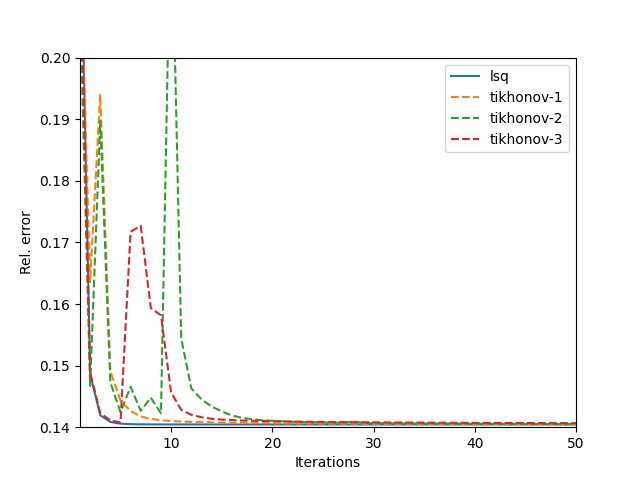
\includegraphics[width=\linewidth]{media/tikhonov-chart.png}
\end{minipage}
\begin{minipage}{0.25\textwidth}
    \centering
\begin{tabular}{l|l}
           & Time  \\ \hline
svd & 1.49s \\
tikhonov-1 & 0.21s \\
tikhonov-2 & 0.21s \\
tikhonov-3 & 0.22s
\end{tabular}
\end{minipage}
    \caption{Comparison between the ALS algorithm when the Tikhonov regularization is used and when not. The dashed lines
    represent different executions of the algorithm and the continuous line represents an iteration of the
    algorithm when using the least squares method for solving \ref{eq:als_lsq}. The TN used
    is a TT with an objective tensor of shape $(8,8,16,8,8)$ and ranks $R = (8,8,8,8)$.
    We can see that
    since in some cases when the linear system is near to zero, the Tikhonov regularization makes the relative
    error skyrocket. With enough iterations the Tikhonov regularization achieves the same
    relative error as the LSQ method. Source: own elaboration.
    Source: own elaboration.}
    \label{fig:als-convergence-tiknov}
\end{figure}
It is also worth noting that from the graph of \figref{fig:als-convergence-tiknov} can't go below
a certain relative error. In this case this value is approximately $0.140439$. This is because the SVD Factorization
method approaches to the solution that minimizes the \gls{LSQ} problem for each core, and as we have seen
it is guaranteed that it minimizes \ref{eq:als_lsq}. 

In practice we will use the Tikhonov regularization for approximating this relative error barrier since it gives us what
is the minimum relative error that we would get with the current \gls{TNS}. In practice, instead 5 iterations of the \gls{SVD} method
we will do 5 iteratios of the Tikhonov regularization method and get the minimum of the relative error that we got during these iterations
since it is way more faster.

% TODO: Potser caldria jugar una mica amb l'algoritme i motivar la següent secció!

\subsection{Backpropagation} \label{backpropagation}

Since our problem of finding tensor cores is defined by minimizing a loss function, a valid idea would be
to apply backpropagation.

In this subsection we will give another way of finding the tensor cores $\mathcal{G}_1, \dots, \mathcal{G}_n$, but with 
backpropagation. The backpropagation algorithm is one of the core algorithms of deep learning. It consists on
trying to find the variation that each parameter does to the loss function by exploiting the chain rule and
then do some optimization with the gradient, such as gradient descent. We will now explain briefly the backpropagation
algorithm in the context of tensor networks.

% (TODO: Citar).

Suppose that we have a set $D$ (a dataset), and a loss function ${\pi: D \times \mathbb{R}^{N_1 \times N_2 \times \cdots \times N_n} \rightarrow \mathbb{R}_+}$
The core idea behind backpropagation is to tune the parameters in a way that
we minimize $\pi_D$. We do this by computing the gradient of all of the parameters of each $\mathcal{G}_i$ and moving 
the parameters in the same direction as the gradient.

In the case that $D = \{T_0\}$ the backpropagation problem is the same as finding the best TNS that represents $T_0$, and if
for example, dataset has more tensors, it can be applied for example as a deep learning problem, as we will see later in chapter 5.

Let $d = T_0$. We want to compute the gradient of
\begin{equation}
\pi(T_0, \mathcal{C}_G(\mathcal{G}_1, \dots, \mathcal{G}_n))
\label{eq:simple-grad}
\end{equation}
Suppose that we reorder $\mathcal{G}_1, \dots, \mathcal{G}_n$ in a sense that the contractions for evaluating the tensor
network become first contracting $\mathcal{G}_n$ and $\mathcal{G}_{n-1}$, then the resulting tensor with $\mathcal{G}_{n-2}$
and so on. The function in $\ref{eq:simple-grad}$ becomes
\begin{equation}
    \pi(T_0, \matchal{C}(\mathcal{G}_1, \mathcal{C}( \mathcal{G}_2, \mathcal{C}(\dots, \mathcal{C}(\mathcal{G}_{n-1}, \mathcal{G}_n))))
    \label{eq:extended-grad}
\end{equation}

Let $X_n = \mathcal{C}(\mathcal{G}_{n-1}, \mathcal{G}_n)$ and let $X_{k} = \mathcal{C}(\mathcal{G}_k, X_{k+1})$ for all $1 \leqslant k \leqslant n - 1$.
We can rewrite \ref{eq:extended-grad} as $\pi(T_0, X_1)$.

We would want to find the derivative of $\mathcal{G}_k$ respect of the loss function $\pi$. Consider the intermidiate
contraction $$X_k = \mathcal{C}(\mathcal{G}_k, X_{k+1})$$
Applying the chain rule we get

\begin{equation}
    \frac{\partial \pi}{\partial \mathcal{G}_k} = \frac{\partial \pi}{\partial X_1} \cdot \frac{\partial X_1}{\partial X_2} \cdots
    \frac{\partial X_{k-1}}{\partial \mathcal{G}_{k}}
\end{equation}

The partial derivative of the core tensor $\mathcal{G}_k$ respect to the loss function tells us in which 

If we want to compute the derivative of the loss function respect to an individual element $\mathcal{G}_k^{i_1, \dots, i_d}$
of the core tensor, using again the chain rule as before we get:

\begin{equation}
    \frac{\partial \pi}{\partial \mathcal{G}_k^{i_1, \dots, i_d}} = \sum_{b_1, \dots, b_m} \frac{\partial \pi}{\partial X_k^{b_1, \dots, b_m}} \cdot 
    \frac{\partial X_k^{b_1, \dots, b_m}}{\partial \mathcal{G}_i^{i_1, \dots, i_d}}
\end{equation}

So, we just have seen that by computing the partials of each intermidiate contraction we can obtain the partial derivative of the loss function
respect to each individual parameter of the core tensor.

After knowing each derivative, we can compute the gradient of $\pi$ in respect to all entries of the core tensors
\begin{equation}
    \nabla \pi = \left( \frac{\partial \pi}{\partial \mathcal{G}_1}, \frac{\partial \pi}{\parital \mathcal{G}_2}, \dots, \frac{\partial \pi}{\partial \mathcal{G}_n} \right)
\end{equation}
With each entry $\displaymath\frac{\partial \pi}{\partial \mathcal{G}_i}$ being a tensor as the same shape of $\mathcal{G}_i$. We can reshape $\nabla \pi$
as a vector of the form
\begin{equation}
    \nabla \pi = \left(\frac{\partial \pi}{\partial \mathcal{G}_1^{a_1, \dots, a_p}}, \dots, \frac{\partial \pi}{\partial \mathcal{G}_n^{b_1, \dots, b_m}} \right)
\end{equation}
Once we computed $\nabla \pi$, now we have an idea that in a local environment, how adjusting each entry of each core tensor affects
on the change of the loss function $\pi$. Let ${w = (\vectorize{\mathcal{G}_1}, \dots, \vectorize{\mathcal{G}_n})}$ be a vector
containing all the entries of the core tensors arrenged in order. Then, we can update each core tensor by "descending" by the
gradient $\nabla \pi$ i.e updating $w$ by a tiny amount on the direction that minimizes the value of the loss function
\begin{equation}
w^* = w - \eta \cdot \nabla \pi(w)
\label{eq:grad-descent}
\end{equation}
Where $\eta$ is a small positive number called the learning rate. If we keep iterating as in \ref{eq:grad-descent}, eventually
$w$ will reach a local minima of the loss function.

We implemented this algorithm using the PyTorch python library, since it has a built-in auto differentiation engine called \verb/torch.autograd/. For 
for every operation that we apply to any PyTorch parameter, it remembers the operations that has been applied to the tensor and then it is able
to compute the gradient of all of our computations \cite{AutomaticDifferentiationTorchautograd}.

% TODO
On \cref{core-finding-algorithms} we can find a comparison between the ALS and the backpropagation algorithms between some tensor network.
As we can observe in
\figref{fig:ap-table-backprop}, on most cases the TN-ALS surpasses the backpropagation
algorithm for finding core tensors with less relative error.

\section{Structure search}

In this section we will describe the TnALE algorithm, that aims to solve problem (\ref{item:problem-2}).

% TODO: Connectar això com deu mana. 
On the last section we supposed that we had found some optimal $G$ and $R$ for representing $T$, and then we 
described some algorithms for finding the cores $\mathcal{G}_1, \dots, \mathcal{G}_n$. In this section,
we will try to find these optimal $(G, R)$.

This problem is known as the \textit{tensor network structure search problem} and its objective 
is to find the most optimal tensor network that 
compresses our objective $T$ while maintaining the expressivity of the network, i.e that the network
is capable to represent a closer result to the actual objective. 

We will define the \textbf{loss function} $\mathcal{L}: \mathbb{G} \times \mathbb{F}_G \rightarrow \mathbb{R}_+$ as
$$\mathcal{L}(G,R) = \phi(G, R) + \lambda \cdot O(G, R) $$
Where $\mathbb{G}$ is the space of all simple connected graphs of $n$ nodes, ${R = (r_1, \dots, r_K) \in \mathbb{F}_G \subseteq
\mathbb{Z}_+^K}$ are the ranks of the tensor network, $\phi(G, R)$ represents a function that determines the complexity of the
tensor network, $\lambda > 0$ is a tuning parameter and $O: \mathbb{G} \times \mathbb{F}_G \rightarrow \mathbb{R}_+$ is the 
\textbf{evaluation function} defined as:
\begin{equation}
    O(G, R) = \min_{\mathcal{Z} \in TNS(G,R)} \pi_D (\mathcal{Z})
    \label{eq:tnale-min-obj}
\end{equation}

We will define the tensor network structure search problem as solving the following discrete optimization problem:
\begin{equation}
    \min_{(G, R) \in \mathbb{G} \times \mathbb{F}_G} \mathcal{L}(G, R)
\label{eq:tnss}
\end{equation}

We can see that minimizing the loss function involves solving a multi-objective minimization problem
since ideally we would want to minimize $\phi$ and $O$. The $\lambda$ parameter applies linear scalarization
for adjusting which solution of the set of the Pareto optimal solutions that our algorithms will want to converge to.

The intuition behind presenting this optimization problem this way is that since the evaluation function depends on the tuning parameter $\lambda$
we can adjust a balance between giving priority to how expressive is the network or on 
simplifying its complexity. We will pich $\phi$ as the \textbf{complexity function} as a function $\phi : \mathbb{G} \times \mathbb{F}_G \rightarrow \mathbb{R}_+$
In our case, we will pick $\phi$ as:

$$\phi(G, R) = \left(\frac{\size(T)}{\size(\mathcal{G}_1) \cdot \size(\mathcal{G}_2) \cdots \size(\mathcal{G}_n)} - 1\right)^{-1}$$

If a candidate structure satisfies that $0 < \size(T) < \size(\mathcal{G}_1) \cdot \size(\mathcal{G}_2) \cdots \size(\mathcal{G}_n)$
then we will directly discard it, since $T$ itself is a better compression. For other values such that $\size(T) > \size(\mathcal{G}_1) \cdots \size(\mathcal{G}_n)$, $O$ is
well defined.

We call the problem \ref{eq:tnss} as Tensor Network Structure Selection (\gls{TN-SS}). TN-SS is a very generalized problem.
There has been a lot of research on solving it under certain conditions:
\begin{itemize}
    \item Tensor Network Rank Selection (\gls{TN-RS}), it restricts $G$ to be a fixed graph, and its objective is to find the
tensor network ranks $R \in \mathbb{F}_G$.
\item Tensor Network Permutation Selection (\gls{TN-PS}) fixes the ranks $R$ and search over the set
of all the simple graphs that are isomorphic to $G$.
\item Lastly, Tensor Network Topology Selection (\gls{TN-TS}) searches over the set of all simple graphs of $N$ vertices and
        the tensor ranks $R$ are fixed
\end{itemize}

In this chapter we will present the tensor network structure search algorithm \gls{TnALE}
introduced by Li et. al. on \cite{liAlternatingLocalEnumeration2023a}.

\subsection{The TnALE algorithm}

The purpose of the \gls{TnALE} algorithm is to solve \ref{eq:tnss} by locally alternating the discrete parameters that define $(G, R)$.

We will start by describing the algorithm itself, and then we will present all the theory for proving its convergence.

The idea behind the TnALE algorithm is very simple: pick a random graph and random ranks $G$ and $R$ and then, for each iteration modifiy
the rank $R_1$ a certain value and then pick the one that minimizes the loss function. Then do the same
for $R_2$ and so on until $R_c$. Then, update $G$ by adding or removing some edges and stay with the structure that is minimizes the loss function.
Then modify $R_c, R_{c_1}, \dots R_2$ as before.

\begin{figure}[H]
    \centering
    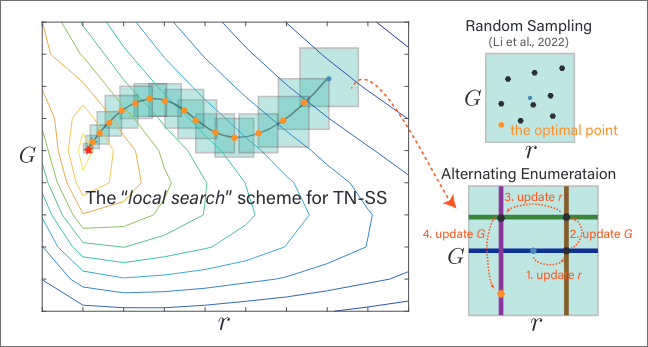
\includegraphics[width=0.75\linewidth]{media/tnale-schema.png}
    \caption{A representation of the TnALE algorithm and the difference of its sampling respect to the \gls{TNLS} algorithm \cite{liPermutationSearchTensor2022}. $r$ and $G$
    denote the structure related variables and each square represents a neighborhood of a given point in the iteration of \gls{TnALE}. Source: \cite{liAlternatingLocalEnumeration2023}}
\end{figure}

Once this first pass is finished, the graph $G$ is modified and each "local neighborhood" of the graph $G$ is evaluated.
Once again we save the best evaluation overwritting $G$ and $R$.

Lastly, we do the first pass of varying the ranks $R_1, \dots, R_c$ but in the reverse order $R_c, \dots, R_1$.
Doing this "round-trip" over the search of the ranks empirically results in a faster convergence rate to the
optimal \gls{TNS} structure.

\begin{figure}[H]
    \centering
\begin{tikzcd}
R_1 \arrow[r] & R_2 \arrow[r]   & \dots \arrow[r] & R_n \arrow[d] \\
R_2 \arrow[u] & \dots \arrow[l] & R_n \arrow[l]   & G \arrow[l]  
\end{tikzcd}
\caption{The "round-trip" of updating the optimal structure. Source: own elaboration}
\end{figure}


\begin{algorithm}[h]
    \caption{Tensor Network Alternating Local Enumeration (Tn-ALE)}

    \hspace*{\algorithmicindent} \textbf{Input}: A starting point $(G^{(0)}, R^{(0)})$ with $R^{(0)} = (R_1^{(0)}, \dots, R_K^{(0)})^T \in \mathbb{Z}_+^K$ 
    and a rank-related radius $r \in \mathbb{Z}_+$ and the number of "round-trips" $D$ \\ 
    \hspace*{\algorithmicindent} \textbf{Output}: The optimal $(G, R)$ that minimizes \refeq{eq:tnss}

    \begin{algorithmic}[1]
        \State Initialize $(G, R) = (G^{(0)}. R^{(0)})$ with $R = (R_1, \dots, R_K)^T$
        \For {$d = 1, \dots D$}
            \For {$k = 1, \dots K$}
                \For {$i = -r, \dots, 0, \dots r$}
                    \State Copy $(\bar{G}, \bar{R}) \leftarrow (G, R)$
                    \State Update $(\bar{G}, \bar{R})$ by $\bar{R_k} = R_k + r$
                    \State $h(i) \leftarrow O(G, R)$ \qquad \verb/# We can apply linear interpolation/
                \EndFor
                \State Update $(G, R)$ by $R_k = \argmin_i h(i)$
            \EndFor
            \State Take the neighborhood of $G$ as $N(G)$
            \ForAll {$G' \in N(G)$}
            % TODO: Aran del futur posa el que has canviat del algoritme
                \State Update $(G, R)$ by $G = G'$ (Insert or delete an element of $R$ if necessary)
                \State $h(G') \leftarrow O(G, R)$
            \EndFor
            \State Update $(G, R)$ by $G = \argmin_{G'} h(G')$
            \For {$k = K, K-1, \dots 2$}
                \For {$i = -r, \dots, 0, \dots r$}
                    \State Copy $(\bar{G}, \bar{R}) \leftarrow (G, R)$
                    \State Update $(\bar{G}, \bar{R})$ by $\bar{R_k} = R_k + r$
                    \State $h(i) \leftarrow O(G, R)$ \qquad  \verb/# We can apply linear interpolation/

                \EndFor
                \State Update $(G, R)$ by $R_k = \argmin_i h(i)$
            \EndFor
        \EndFor
        \State \Return $(G, R)$

    \end{algorithmic}

    \label{alg:tn-ale}
\end{algorithm}

In Alg. \ref{alg:tn-ale} the pseudocode of \gls{TnALE} is given. During the next subsection, we will need to introducte some theory of
gradient-less optimization for proving the convergence of the \gls{TnALE} algorithm.

Keep in mind that for each time we try to vary some rank $R_k$ or the graph $G$ we will need to evaluate \eqref{eq:tnale-min-obj}, and it 
can be computationally very expensive. In the case that we are varying a rank (See steps 7 and 21 of Alg. \ref{alg:tn-ale}), we can 
approximate $O(G, R)$ by doing a linear interpolation between evaluating at the points
$R_k - r, R_k, R_k + r$. Since by increasing ranks empirically yields 
to a better representation of the objective tensor \cite{liAlternatingLocalEnumeration2023} and therefore we get less relative error
(and the other way around is generally also true).

We will now formally prove that the \gls{TnALE} algorithm converges. For that, we will need to introduce the gradientless descent.

\subsection{Gradientless optimization}

What we want to see in this subsection is to extend the notion of the gradient onto 
discrete functions to then be able to apply a discrete gradient descent over our loss function.

We will start by rewriting the loss function \eqref{eq:tnss} in a more general form. We define $\mathbb{P}$ as the
set of all functions of the form $p : \mathbb{Z}_+^K \rightarrow \mathbb{K}_+^L$
\begin{equation}
\min_{x \in \mathbb{Z}_+^K, p \in \mathbb{P}} f_p(x) := f \circ p(x)
\label{eq:min_grad}
\end{equation}
Where $f_p : \mathbb{Z}_+^L \rightarrow \mathbb{R}_+$ is a generalization of the loss function, and $p : \mathbb{Z}_+^K \rightarrow \mathbb{Z}_+^L \in \mathbb{P}$
correspond to the topology-related variable $(G, R)$.

We can show that our tensor network structure search problem corresponds to a concrete case of this general form: since $G$ is completly defined by its adjacency matrix $A$ which is defined as
$$A_{ij} := \begin{cases}
    1 & \text{if }\;(i, j) \in E \\
    0 & \text{otherwise}
\end{cases}$$
We can encode the ranks $R$ on the adjacency matrix by setting on each edge its corresponding rank:
$$A_{ij} := \begin{cases}
    R_{(i,j)} & \text{if}\;(i, j) \in E \\
    0 & \text{otherwise}
\end{cases}$$
Where $R_{(i,j)}$ denotes the rank of the edge $(i.j)$. We will denote this matrix as $A_R$

\begin{example}
    Let $G = P_4$ and $R = (1,2,3)$. We associate the edges of $G$ with the ranks $R$ as
    $R_{(1, 2)} = r_1 = 1$, $R_{(2, 3)} = r_2 = 2$ and $R_{(3, 4)} = r_3 = 3$. We consider $\TNS(G; R)$.
    The adjacency matrix of $G$ and the encoded rank matrix of $\TNS(G;R)$ is, respectively:
    $$A = \begin{pmatrix}
        0 & 1 & 0 & 0 \\
        1 & 0 & 1 & 0 \\
        0 & 1 & 0 & 1 \\
        0 & 0 & 1 & 0 \\
    \end{pmatrix} \qquad
    A_R = \begin{pmatrix}
        0 & 1 & 0 & 0 \\
        1 & 0 & 2 & 0 \\
        0 & 2 & 0 & 3 \\
        0 & 0 & 3 & 0 \\
    \end{pmatrix}$$
\end{example}

Given $G$ and $R$, we can encode $x \in \mathbb{R}_+^K$ as a vector with the rank of each edge of the graph and
$p \in \mathbb{P}$ as a permutation matrix. By varying only $p$ we get all the permutations of the graph $G$, 
and by $x$ we get vary the ranks of the edges.

\begin{example}
\iffalse
$$A^1_R = \begin{pmatrix}
    0 & {\color{teal} 1} & {\color{teal} 0} & {\color{teal} 0} \\
    1 & 0 & {\color{teal}2} & {\color{teal} 0} \\
0 & 2 & 0 & {\color{teal}3} \\
        0 & 0 & 3 & 0 \\
    \end{pmatrix} \Leftrightarrow p_1(x) = \begin{pmatrix}
        1 & 0 & 0 & 0 & 0 & 0 \\
        0 & 1 & 0 & 0 & 0 & 0 \\
        0 & 0 & 1 & 0 & 0 & 0 \\
        0 & 0 & 0 & 1 & 0 & 0 \\
        0 & 0 & 0 & 0 & 1 & 0 \\
        0 & 0 & 0 & 0 & 0 & 1 \\
        \end{pmatrix} \begin{pmatrix}
        1 \\ 0 \\ 0 \\ 2 \\ 0 \\ 3
        \end{pmatrix} = \begin{pmatrix}
        1 \\ 0 \\ 0 \\ 2 \\ 0 \\ 3
    \end{pmatrix}$$

$$A^2_R = \begin{pmatrix}
    0 & {\color{teal}0} & {\color{teal}0} & {\color{teal}3} \\
    0 & 0 & {\color{teal}1} & {\color{teal}0} \\
    0 & 1 & 0 & {\color{teal}2} \\
        3 & 0 & 2 & 0 \\
    \end{pmatrix} \Leftrightarrow p_1(x) = \begin{pmatrix}
        0 & 0 & 0 & 1 & 0 & 0 \\
        0 & 1 & 0 & 0 & 0 & 0 \\
        0 & 0 & 0 & 0 & 1 & 0 \\
        0 & 0 & 0 & 0 & 0 & 1 \\
        1 & 0 & 0 & 0 & 0 & 0 \\
        0 & 0 & 1 & 0 & 0 & 0 \\
        \end{pmatrix} \begin{pmatrix}
        1 \\ 0 \\ 0 \\ 2 \\ 0 \\ 3
        \end{pmatrix} = \begin{pmatrix}
        0 \\ 0 \\ 3 \\ 1 \\ 0 \\ 2
    \end{pmatrix}$$
    \label{ex:graph-k-correspondance}
\fi

$$A^1_R = \begin{pmatrix}
    0 & {\color{teal} 1} & {\color{teal} 0} & {\color{teal} 0} \\
    1 & 0 & {\color{teal}2} & {\color{teal} 0} \\
0 & 2 & 0 & {\color{teal}3} \\
        0 & 0 & 3 & 0 \\
    \end{pmatrix} \Longleftrightarrow p_1(x) = \begin{pmatrix}
        1 & 0 & 0 & 2 & 0 & 3
    \end{pmatrix}^T$$

$$A^2_R = \begin{pmatrix}
    0 & {\color{teal}0} & {\color{teal}0} & {\color{teal}3} \\
    0 & 0 & {\color{teal}1} & {\color{teal}0} \\
    0 & 1 & 0 & {\color{teal}2} \\
        3 & 0 & 2 & 0 \\
    \end{pmatrix} \Longleftrightarrow p_1(x) =
        = \begin{pmatrix}
        0 & 0 & 3 & 1 & 0 & 2
    \end{pmatrix}$$
    \label{ex:graph-k-correspondance}
\end{example}

So, our problem is now a particular case of \eqref{eq:min_grad}. We can now apply theory of gradientless
optimizations in the real domain.


% TODO: moure

The goal of this section is to try to extend the gradient and its properties into discrete valued functions $f: \mathbb{Z}_+^L \rightarrow \mathbb{R}$.
It is based on the theory that Golovin et. al. present on \cite{golovinGradientlessDescentHighDimensional2019}, and also on the discussion
of the \gls{TnALE} algorithm itself in the appendix of \cite{liAlternatingLocalEnumeration2023}.
We will end this chapter by proving that if we take some assumptions of $f$ like 
being convex and also smooth we can prove that the \gls{TnALE} algorithm can converge. For that, we will define what
is a discrete gradient, what is $\alpha$-strong convergence and $(\beta_1, \beta_2)$-smoothness, we will prove some properties
about strong convergence and smoothness.

% TODO: Omplir amb que faràs més endavant en aquesta secció.
Before we begin, since we will be working with vectors of $\mathbb{Z}_+^L$, we will introduce a norm for them:
\begin{definition}
    The $l^2$ norm of a vector $x = (x_1, \dots, x_n)^T$ is defined as
    $$ \|x\|_2 = \sqrt{\sum_{i=1}^n |x_i|^2}$$
\end{definition}

From now on, if $x$ is a vector we will represent $\|x\|$ as $\|x\|_2$. We can now start by defining the concept of finite gradient:

\begin{definition}
    For any function $f: \mathbb{Z}_+^L \rightarrow \mathbb{R}$ its finite gradient $\nabla f : \mathbb{Z}_+^L \rightarrow \mathbb{R}$ at a point
    $x \in \mathbb{L}_+^L$ is defined as
    $$\Delta f(x) = [ f(x + e_1) - f(x), \dots, f(x + e_L) - f(x) ]^T$$
\end{definition}

With $e_i$ being the unit vector of $\mathbb{Z}_+^L$ defined with the $i$-th entry being $1$ and the rest of entries zeros.

% TODO: Afegir drawing del que es un finite gradient

\begin{lemma}
    Let $x \in \mathbb{Z}_+^L$. Then $\Delta \|x\|_2^2 = 2x + \textbf{1}$ where $\textbf{1}$ denotes the unit vector of $\mathbb{Z}_+^L$ that all of its entries are $1$.
    \begin{proof}
        $$\Delta \|x\|_2^2 = \Delta \left( \sum_{i=1}^L |x_i|^2 \right) = \sum_{i=1}^L \Delta |x_i|^2 = \sum_{i=1}^L 2 x_i + e_i = 2 x + \textbf{1}$$
        Where in the penultimate equality we used that
        $$\Delta |x_i|^2 = |x_i + e_i|^2 - |x_i|^2 = |x_i|^2 + 2 \langle x_i, e_i \rangle + |e_i|^2 - |x_i|^2 = 2 \langle x_i, e_i \rangle + e_i = 2x_i + e_i$$
    \end{proof}
\end{lemma}

Now we will extend the strong convexity using the finite gradient. Recalling, a differentiable function $f: X \subseteq \mathbb{R}^n \rightarrow \mathbb{R}$ is 
convex if and only if for all $x, y \in X$
$$f(y) \geqslant f(x) - \langle \Delta f(x), y - x \rangle$$
Where $\Delta f(x)$ denotes the gradient of $f$. If $f$ also satisfies that
\begin{equation}
f(y) \geqslant f(x) + \langle \Delta f(x) - \frac{\alpha}{2} \textbf{1}, y - x \rangle + \frac{\alpha}{2} \|y - x\|^2_2
\label{eq:strong-convex}
\end{equation}
For some $\alpha \geqslant 0$ e say that $f$ is $\alpha$-strongly convex.
\begin{definition}
    We say that $f: \mathbb{Z}_+^L \rightarrow \mathbb{R}$ is $\alpha$-strongly convex with $\alpha \geqslant 0$ if it
    satisfies \refeq{eq:strong-convex} with $\Delta f(x)$ being the finite gradient for all $x, y \in \mathbb{Z}_+^L$ if the
    inequality holds for $\alpha = 0$, we will say that $f$ is convex.
\end{definition}
We will prove now some properties of $\alpha$-strongly convex functions. The following lemma
gives us the equivalence between $\alpha$-stronglt convex functions and convex functions:
\begin{lemma}
    $f : \mathbb{Z}_+^L$ is an $\alpha$-strongly convex function iff $g(x) = f(x) - \displaymath\frac{\alpha}{2} \|x\|^2_2$ is convex $\forall x \in \mathbb{Z}_+^L$
    \begin{proof}
        $(\Rightarrow)$ The first statement is equivalent to proving
        \begin{equation}
            g(y) \geqslant g(x) + \langle \Delta g(x), y - x \rangle \quad \forall x, y \in \mathbb{Z}_+^L
            \label{eq:g-lemma-sconv}
        \end{equation}
        Applying that $f(x)$ is $\alpha$-strongly convex we get that
        \begin{align*}
            g(y) - g(x) - & \langle \Delta g(x), y - x \rangle = f(y) - \frac{\alpha}{2}\|y\|^2_2 - f(x) + \frac{\alpha}{2}\|x\|^2_2 - \langle \Delta g(x), y - x \rangle \\
                          & = f(y) - \frac{\alpha}{2}\|y\|^2_2 - f(x) + \frac{\alpha}{2}\|x\|^2_2 - \langle \Delta f(x) - \alpha (2x + \textbf{1}), y - x \rangle \\
                          & = f(y) - f(x) - \langle \Delta f(x) - \frac{\alpha}{2} \textbf{1}, y - x \rangle - \frac{\alpha}{2}\|y\|_2^2 + \frac{\alpha}{2}\|x\|_2^2 + \frac{\alpha}{2} \langle 2x, y - x \rangle \\
                          & \geqslant \frac{\alpha}{2} \|y-x\|_2^2 - \frac{\alpha}{2} \|y\|_2^2 + \frac{\alpha}{2} \|x\|_2^2 + \frac{\alpha}{2} \langle 2x, y - x \rangle \\
                          & = \frac{\alpha}{2} \left( \|y-x\|^2_2 - \|y\|_2^2 - \|x\|_2^2 + 2\langle x, y \rangle \right) = 0
        \end{align*} 

        $(\Leftarrow)$ From \refeq{eq:g-lemma-sconv} we get
        \begin{align*}
            & f(y) - \frac{\alpha}{2} \|y\|_2^2 \geqslant f(x) - \frac{\alpha}{2} \|x\|_2^2 + \langle \Delta f(x) - \frac{\alpha}{2} (2x + \textbf{1}) , y - x \rangle \\
            \Leftrightarrow \; & f(y) \geqslant f(x) - \frac{\alpha}{2} (\|x\|_2^2 + \|y\|_2^2) + \langle \Delta f(x) - \frac{\alpha}{2} \textbf{1}, y - x \rangle - \frac{\alpha}{2} \langle 2x, y - x \rangle \\
            \Leftrightarrow \; & f(y) \geqslant f(x) + \langle \Delta f(x) - \frac{\alpha}{2} \textbf{1}, y - x \rangle + \frac{\alpha}{2}\|y - x\|^2_2
        \end{align*}
        The last inequality gives us that $f$ is $\alpha$-strongly convex.
    \end{proof}
    \label{lem:g-convex}
\end{lemma}


The following lemma tells us that $\alpha$-strongly convex functions have a more strict inequality of the
monotone gradient property (a function is convex iff its gradient is monotone) than convex functions. 
\begin{lemma}
    Given $f$ an $\alpha$-strongly convex function in $\mathbb{Z}_+^L$, then:
    \begin{enumerate}
        \item $\langle \Delta f(x) - \Delta f(y), x - y \rangle \geqslant \alpha \|x - y\|^2_2 \quad \forall x, y \in \mathbb{Z}_+^L$
        \item $\|\Delta f(x) - \Delta f(y)\|_2 \geqslant \alpha \|x - y\|_2 \quad \forall x, y \in \mathbb{Z}_+^L$
    \end{enumerate}
    \begin{proof}
        Let $g(x)$ be the same as in \lemref{lem:g-convex}. To prove $(1)$, we know that 
        $$\langle \Delta g(x) - \Delta g(y), x - y \rangle \geqslant 0, \forall x, y \in \mathbb{Z}^L_+$$ by the monotone gradient property
        of the convexity, which is true in both continuous and discrete scenarios. By substituting $\Delta g(x)$ we get that
        $$ \langle \Delta f(x) - \frac{\alpha}{2} (2x + \textbf{1}) - \Delta f(y) + \frac{\alpha}{2}(2y + \textbf{1}), x - y \rangle \geqslant 0$$
        Simplifying we obtain that for all $x, y \in \mathbb{Z}_+^L$
        \begin{equation}
            \langle \Delta f(x) - \Delta f(y), x - y \rangle \geqslant \alpha \|x- y\|^2_2
            \label{eq:grad-monotony}
        \end{equation}
        For proving (2) Consider the following inequality:
        $$\|\Delta f(x) - \Delta f(y)\|_2 \|x - y\|_2 \geqslant \langle \Delta f(x) - \Delta f(y) , x - y \rangle \geqslant \alpha \|x- y\|^2_2$$
        Where in the first inequality we used the Cauchy-Swartz inequality and the last inequality follows from \eqref{eq:grad-monotony}
    \end{proof}
\end{lemma}



The following lemma tells us that if we have a $\beta$-Lipschitz discrete function, the gradient is bounded. This
will be one of the main assumptions that we will make about our loss function.
\begin{lemma}
    If $\|f(x) - f(y)\|_2 \leqslant \beta \|x - y\|$ for all $x, y \in \mathbb{Z}_+^L$ then the norm of the finite gradient
    is bounded by $\beta$ i.e $\|\Delta f(x)\|_\infty = \max(|\Delta f(x)_1|, \dots, |\Delta f(x)_L|) \leqslant \beta$
    \begin{proof}
        Denote $\Delta f(x)_i$ the $i$-th entry of $\Delta f(x)$. Then for all $1 \leqslant i \leqslant L$,
        $$|\Delta f(x)_i| = |f(x + e_i) - f(x)| \leqslant \beta \|x + e_i - x \| = \beta$$
    \end{proof}
\end{lemma}

\begin{definition}
    We say $f$ is $(\beta_1, \beta_2)$-smooth for $\beta_1, \beta_2 > 0$ if
    \begin{enumerate}
    \item $|f(x) - f(y)| \leqslant \beta \|x - y\|_2$ for all $x, y \in \mathbb{Z}_+^L$
    \item The function $l(x) := \frac{\beta_2}{2} \|x\|^2_2 - f(x)$ is convex
    \end{enumerate}
\end{definition}

The first item makes $f$ to a $\beta_1$-Lipschitz function implying the "continuity" of the function, while the second
item ensures an upper bound to the change of the gradient, because of the following lemma:
\begin{lemma}
    If $l(x) = \frac{\beta_2}{2} \|x\|^2_2 - f(x)$ is convex, then $\forall x, y \in \mathbb{Z}_+^L$ the following
    inequality satisfies:
    $$ \langle \Delta f(x) - \Delta f(y), x - y \rangle \leqslant \beta \| x - y \|^2_2 $$
    \begin{proof}
        By the convexity of $l(x)$ we get that
        $$l(y) \geqslant l(x) + \langle \Delta l(x), y - x \rangle$$
        Similarly we get
        $$l(x) \leqslant l(y) + \langle \Delta l(y), x - y \rangle$$
        Summing the two inequalities, we get that
        $$l(y) + l(x) \geqslant l(x) + l(y) + \langle \Delta l(y) - \Delta l(x), x - y \rangle$$
        And therefore
        $$\langle \Delta l(x) - \Delta l(y), x - y \rangle \geqslant 0$$
        Applying $l(x)$ we get that
        $$ \langle \beta(2x + \textbf{1}) - \Delta f(x) - \beta(2y + \textbf{1}) + \Delta f(y), x - y \rangle \geqslant 0$$
        And by simplifying the inequality we have that
        $$\langle \Delta f(x) - \Delta f(y), x - y \rangle \leqslant \beta \|x - y\|_2^2$$
    \end{proof}
\end{lemma}
\subsection{Proof of the convergence of the TnALE algorithm}

After presenting $\alpha$-strongly convex functions and $(\beta_1, \beta_2)$-smooth functions, in this
subsection we will now prove that by setting the assumptions that our original problem from \ref{eq:min_grad}
the function $f_p$ is $\alpha$-strongly convex and $(\beta_1, \beta_2)$-smooth with $0 \leqslant \alpha \leqslant \beta_1 \leqslant \beta_2 \leqslant 1$ and
that the minimum point of the discrete gradient which will be a fixed point of the \gls{TnALE} algorithm does in fact exists and
that its gradient is bounded by a very small factor.

We will start by defining the sub-level set of a function at a point. This definition will be useful for
later proving that the \gls{TnALE} algorithm can descend:

\begin{definition}[Sub-level set] The level set of $f$ at a point $x \in \mathbb{Z}_+^L$ is defined as
    the set $\mathbb{L}_x(f) = \{y \in \mathbb{Z}_+^L : f(y) = f(x)\}$ The sub-level set of $f$ at a point
    $x$ is defined as the set $\mathbb{L}_x^{\downarrow} = \{y \in \mathbb{Z}_+^L : f(y) \leqslant f(x) \}$
\end{definition}


Now, with the following lemma we will see that we can always find a neighbourhood that is contained
inside $\mathbb{L}_x^\downarrow$, this will mean that we would be able to find a succession of points $(x_n)_{n=1}^\infty$ such
that each $f(x_i) \leqslant f(x_j)$ if $i > j$

\begin{lemma}
    Let $f : \mathbb{Z}_+^L \rightarrow \mathbb{R}$ be a $\alpha$-strongly convex, $(\beta_1, \beta_2)$-smooth and
    that its minimum value $f(x^*)$ satisfies that $\|\frac{\beta_2}{2} \textbf{1} - \Delta f(x^*)\| \leqslant \gamma$ where
    $\gamma$ is a constant and $0 \leqslant \gamma \leqslant \alpha$. Then $\forall x \in \mathbb{Z}_+^L$ there exists
    a $L$-dimensional cube which is of edge length $\frac{2(\alpha - \gamma)}{\beta_2 \sqrt{L}} \|x - x^*\|$, tangent at
    $x$ and inside the sub-level set $\mathbb{L}_x^\downarrow (f)$
    \label{lem:cube}
\end{lemma}
The proof of this lemma can be found at lemma B.8 from the appendix of \cite{liAlternatingLocalEnumeration2023}
\begin{lemma}[Convex combination in the discrete domain]
    Suppose that $q = \theta x + (1 - \theta) y$ for all $x, y \in \mathbb{Z}_+^L$ and $\theta \in [0,1]$ and that
    there is a $\hat q \in \mathbb{Z}^L_+$ such that if $\Lambda = q - \hat q$ and we suppose that $f$ is $\alpha$-strongly convex then
    $$\theta f(x) + (1 - \theta)f(y) \geqslant f(\hat q) + \langle \Delta f(\hat q) - \frac{\alpha}{2}\textbf{1}, \Lambda \rangle + \frac{\alpha}{2} \|\Lambda\|^2_2$$
    \label{lem:convex-combi}
\end{lemma}

% TODO: ?
Note that this lemma justifies that we can use the linear interpolation trick when evaluating tensor networks, since
by picking $\hat q$ as the local minimum when varying one parameter of the rank $R_i$, since we are moving across one line
all of our real evaluations that we are skipping will be bounded below our linear interpolation.
    \begin{proof}
        By the definition of the $\alpha$-strong convexity we get
        $$f(x) \geqslant f(\hat q) + \left\langle \Delta f(\hat q) - \frac{\alpha}{2}\textbf{1}, x - \hat q \right\rangle + \frac{\alpha}{2} \| x - \hat q \|^2_2$$
        $$f(y) \geqslant f(\hat q) + \left\langle \Delta f(\hat q) - \frac{\alpha}{2}\textbf{1}, y - \hat q \right\rangle + \frac{\alpha}{2} \| y - \hat q \|^2_2$$
        And therefore,
        \begin{align*}
            \theta f(x) + (1 - \theta) f(y) &\geqslant f(\hat q) + \left\langle \Delta f(\hat q) - \frac{\alpha}{2} \textbf{1}, \Lambda  \right\rangle +
        \frac{\alpha}{2} (\theta \|x\|^2 + (1- \theta) \|y\|^2 + \|\hat q\|^2 - 2 \langle q, \hat q \rangle ) \\
                                            &\geqslant f(\hat q) + \left\langle \Delta f(\hat q) - \frac{\alpha}{2} \textbf{1}, \Lambda \right\rangle
                                            + \frac{\alpha}{2} (\|q\|^2 + \|\hat q\|^2 - 2\langle q, \hat q \rangle) \\
                                            &= f(\hat q) + \left\langle \Delta f(\hat q) - \frac{\alpha}{2} \textbf{1}, \Lambda \right\rangle + \frac{\alpha}{2} \|\Lambda\|^2
        \end{align*}
    \end{proof}

\begin{theorem}
    Let $f: \mathbb{Z}_+^K \rightarrow \mathbb{R}_+$ is $\alpha$-strongly convex, $(\beta_1, \beta_2)$-smooth
    and let the minimum of \refeq{eq:min_grad} be $(p^*, x^*)$. Assume that $f$ satisifies $\| \Delta f_{p^*} (x^*) - \frac{\beta_2}{2} \textbf{1} \|_2 \leqslant \gamma$
    where $0 \leqslant \gamma < \alpha \leqslant \beta_1 \leqslant \beta_2 \leqslant 1$.

    Then, if we let $p$ fixed as $p^*$, and $0 \leqslant \theta \leqslant 1$ and for any $x$ with $\|x - x^*\|$_\infty \leqslant c$
    we can find a neighborhood $B_\infty (x, r_X)$ where $r_X \geqslant \theta c + \frac{1}{2}$ such that there exists an element
    $y \in B_\infty (x, r_X)$ satisfying
    $$f_{p^*}(y) - f_{p^*}(x^*) \leqslant (1 - \theta) (f_{p^*}(x) - f_{p^*}(x^*)) + \frac{7}{8}K$$
    \label{thm:ale-convergence}
\end{theorem}
\begin{proof}
    Since we are letting $p$ to be fixed as $p^*$, the general problem
$\displaymath\min_{x \in \mathbb{Z}_+^K, p \in \mathbb{P}} f_p(x)$ can be simplified and equivalently rewritten as $\displaymath\min_{x \in \mathbb{Z}_+^K} f(x)$
Where $f: \mathbb{Z}^K_+ \rightarrow \mathbb{R}_+$ represents the objective function.
By \lemref{lem:convex-combi} we have
$$f(\hat q) - f(x^*) \leqslant (1 - \theta) (f(x) - f(x^*)) + \left\langle \frac{\alpha}{2} \textbf{1} - \Delta f(\hat q), \Delta \right\rangle - \frac{\alpha}{2} \|\Delta \|^2
$$
Now we will see that there exists an element $y$ inside a neighborhood $B(x, r_x)$ with $r_x \in \mathbb{R}_+$ such that $y$
also belongs to the sub-level cube tangent at $\hat q$ from \lemref{lem:cube} so that the inequality $f(y) \leqslant f(\hat q)$ holds.
We will prove the existance of this point $y$ by showing that the intersection
between the sub-level cube tangent at $\hat q$ and $B(x, r_x)$ is not empty. For that
we will find the distance between $\hat q$ and $x$ satisfies that
$$\|x - \hat q\|_\infty = \|x - q + \Lambda\|_\infty \leqslant \| x - q \|_\infty + \| \Lambda \|_\infty = 
\theta \|x - x^*\|_\infty + \|\Lambda \|_\infty \leqslant \theta c + \frac{1}{2}
$$
The last inequality follows from $\|\Lambda \| \leqslant \frac{1}{2}$ which holds because we can always find $\hat q \in \mathbb{Z}_+^K$ by
rounding the entries of $q$ to its closest integers. Therefore we have proven that if $r_x \geqslant \theta c + \frac{1}{2}$ the intersection of the 
sub-level cube tangent at $\hat q$ and $B(x, r_x)$ is not empty, proving the existance of the point $y$.

Lastly, if we take an element $y$ from the intersection we get that
\begin{align*}
    f(y) - f(x^*) &\leqslant f(\hat q) - f(x^*) \leqslant (1 - \theta) (f(x) - f(x^*)) + \left\langle \frac{\alpha}{2} \textbf{1} - \Delta f(\hat q), \Lambda \right\rangle - \frac{\alpha}{2} \| \Lambda \|^2 \\
                  &\leqslant (1 - \theta) (f(x) - f(x^*)) + \left| \left\langle \frac{\alpha}{2} \textbf{1}, \Lambda \right\rangle \right| + |\langle \Delta f(\hat q), \Lambda \rangle| + \frac{\alpha}{2} \| \Lambda \|^2 \\
                  &\leqslant (1 - \theta) (f(x) - f(x^*)) + \frac{\alpha}{4} K + \| \Delta f(\hat q) \|_\infty \| \Lambda \|_1 + \frac{\alpha}{2} \|\Lambda \|^2 \\
                  &\leqslant (1 - \theta) (f(x) - f(x^*)) + \frac{\alpha}{4}K + \frac{\beta_1}{2}K + \frac{\alpha}{8} K \\
                  &\leqslant (1-\theta) (f(x) - f(x^*)) + \frac{3\alpha + 4\beta_1}{8}K \\
                  &\leqslant (1-\theta) (f(x) - f(x^*)) + \frac{7}{8} K
\end{align*}
The inequality of the fourth line follows from $\|\Delta f(x)\|_\infty \leqslant \beta_1$ and from $\|\Lambda \|_\infty \leqslant \frac{1}{2}$
and the last line comes from that $\alpha \leqslant \beta_1 \leqslant 1$
\end{proof}

The assumption of the satisfaction of the 
inequality $\|\Delta f_{p^*}(x^*) - \frac{\beta_2}{2} \textbf{1}\|_2 \leqslant \gamma$ implies that
$\Delta f_{p^*}(x^*)$ should be sufficiently smaller than the constant vector $\frac{\beta_2}{2} \textbf{1}$, which
can be understood as a discrete version of the zero-gradient stationary points of the continuous domain.

The constant $K$ that appears on the proof is due to the fact that $\|\Lambda \|_1 \leqslant K\|\Lambda \|_\infty \leqslant K/2$ and that
$\|\Lambda\|_2 \leqslant K\|\Lambda \|_\infty \leqslant \sqrt{K}/2$. This gives us that the norms $\|\Lambda \|_1$ and $\|\Lambda \|_2$ can become
larger as the dimension $K$ grows, which it is inevitable except if $\|\Lambda \|_\infty=0$, which implies as we defined $\Lambda$ the conventional
convex optimizitation over the continuous domain.

Keeping all of the assumption of $f$, we can prove that local sampling methods, in concrete, \gls{TnALE} converges:
\begin{corollary}
    Let $(x_n)_{n=0}^\infty$ be a succession of $\mathbb{Z}_+^K$ with $x_0$ randomly chosen. Suppose that $p^*$ is known and
    that $x_n$ is equal to the $y$ of \thmref{thm:ale-convergence} for all $n> 0$. Then, if $\Omega(1/K) \leqslant \theta \leqslant 1$, i.e
    $\theta$ scales at least as $1/K$, we have that
    $$\lim_{n \to \infty} (f_{p^*} (x_n) - f_{p^*}(x^*)) = O(1)$$
    \begin{proof}
        Let $C_K = (7/8)K$. By \thmref{thm:ale-convergence},
        \begin{align*}
            f_{p^*}(x_n) - f_{p^*}(x^*) &\leqslant (1- \theta) (f_{p^*} (x_{n-1}) - f_{p^*}(x^*)) + C_K \\
                                        &\leqslant (1 - \theta)^2 (f_{p^*}(x_{n-2}) - f_{p^*}(x^*)) + C_K + C_K(1 - \theta) \\
                                        &\leqslant (1 - \theta)^3 (f_{p^*}(x_{n-3}) - f_{p^*}(x^*)) + C_K + C_K(1 - \theta) + C_K(1- \theta)^2 \\
                                        &\leqslant \dots \\
                                        &\leqslant (1-\theta)^n (f_{p^*}(x_{0}) - f_{p^*}(x^*)) + C_K \sum_{m=1}^n (1 - \theta)^{m - 1}
        \end{align*}
        Using that $\Omega(1/K) \leqslant \theta \leqslant 1$ we get that
        $$\lim_{n \to \infty} (f_{p^*}(x_n) - f_{p^*}(x^*)) \leqslant \lim_{n \to \infty} (1 - \theta)^n (f_{p^*}(x_0) - f_{p^*}(x^*))+ C_K \sum_{m=1}^n (1 - \theta)^{m-1}$$
        $$ = 0 + C_K \frac{1}{\theta} = K \frac{7}{8 \theta} \leqslant O(1)$$
        Since in the last equality the term $\theta$ scales at least as $1/K$, therefore everything does not scale
        depending in $K$ or $\theta$, making the limit converge to some constant.
    \end{proof}
\end{corollary}

And with this corollary we have proven that the \gls{TnALE} algorithm converges. On the last corollary we have taken in account that $K$ could also grow during
the limit. In our case $K$ would be the fixed value of our dimension that depends on the number of nodes from the graph space $\mathbb{G}$ that we are
considering (See \exref{ex:graph-k-correspondance}).

In this chapter we have seen how to search optimal structures of tensor networks that guarantee that
when we search the optimal cores these minimize a loss function $\pi_D$. For achieving this we have
seen first that if we fix the tensor network structure to some graph and ranks $(G, R)$ we can 
apply the TN-ALS algorithm or we can use backpropagation for obtaining the cores
$\mathcal{G}_1, \dots, \mathcal{G}_n$ that minimize the loss function fixed $(G, R)$.

Then, we have presented the TnALE algorithm, which objective is to give a general solution to the
\gls{TN-RS}, \gls{TN-PS} and \gls{TN-TS} problems, giving us an optimal tensor network structure $(G, R)$ and saving
some evaluations when testing for tensor network structure candidates.

Finally, we have proved that under certain assumptions about the loss function, the TnALE algorithm
does converge to a certain structure. We have presented gradientless optimization theory to prove this fact.

On the following chapter we will see some applications of all of these algorithms combined. We will use them
to compress some images and we will also use them for compressing the weights of fully connected neural network layers.

\iffalse
\section{Evaluation function}

The last piece on our algorithm is now how to evaluate our loss function from \refeq{eq:loss_function}.
In this section we will try to give a good approximation of
$$\min_{\mathcal{Z} \in \TNS(G,R)} \pi_D (\mathcal{Z})$$
fixed some $G \in \mathbb{G}$ and $R \in \mathbb{F}_G$.
\fi


% TODO:
% Suposo que començar per dir quines parts del graf caldria tallar maybe???
% Fer més representacions gràfiques de segons quina demostració com més clar quedi tot millor
% \begin{itemize}
% \item Descriure $G$-ranks
% \item Algorismes per aproximar TNS per $G$-ranks propers i mínims si es pot fer
% \item Algun algorisme per trobar heuristicament els $G$-ranks adequats? (suposo q depen de compressió ratio i l'error relatiu)
% \item Com podem trobar un $G$ adequat?
% \item Estratègies per contraure tensors més ràpidament? (DRMG?)
% \item Algorismes, part pràctica en C/C++
% \item Fer moltes gràfiques
% \item Fer aplicacions per machine learning, etc.
% \item Fixar la mathematical subject classification
% \end{itemize}

\chapter{Applying TN low-rank approximations on FCNN}

\section{Neural networks}


Neural networks are modeled after how real neurons work, but in a simplified manner \cite{ExplainedNeuralNetworks2017}: each neural network contains a set of neurons which are split in
different layers. A fully connected neural network is composed on 3 different parts: an \textbf{input layer}, a central part with some layers 
called \textbf{hidden layers} and an \textbf{output layer}. The idea of neural networks is that they recieve an encoded input through
the input layer and this input will be successively processed by the hidden layers and then it will return a certain result
through the output layer. (See \figref{fig:fcnn})

\begin{figure}[H]
    \centering
    \begin{tikzpicture} 

    \node(i2)[draw, shape=circle, minimum size=0.5cm] at (0,-1) {};
    \node(i3)[draw, shape=circle, minimum size=0.5cm] at (0,0) {};
    \node(i4)[draw, shape=circle, minimum size=0.5cm] at (0,1) {};
    \node(i5)[draw, shape=circle, minimum size=0.5cm] at (0,2) {};
    \node(i6)[draw, shape=circle, minimum size=0.5cm] at (0,3) {};
    \node(i7)[draw, shape=circle, minimum size=0.5cm] at (0,4) {};

    \node(l2)[draw, shape=circle, minimum size=0.5cm] at (2,3) {};
    \node(l3)[draw, shape=circle, minimum size=0.5cm] at (2,2) {};
    \node(l4)[draw, shape=circle, minimum size=0.5cm] at (2,1) {};
    \node(l5)[draw, shape=circle, minimum size=0.5cm] at (2,0) {};

    \node(p2)[draw, shape=circle, minimum size=0.5cm] at (4,3) {};
    \node(p3)[draw, shape=circle, minimum size=0.5cm] at (4,2) {};
    \node(p4)[draw, shape=circle, minimum size=0.5cm] at (4,1) {};
    \node(p5)[draw, shape=circle, minimum size=0.5cm] at (4,0) {};

    \node(o2)[draw, shape=circle, minimum size=0.5cm] at (6,-1) {};
    \node(o3)[draw, shape=circle, minimum size=0.5cm] at (6,0) {};
    \node(o4)[draw, shape=circle, minimum size=0.5cm] at (6,1) {};
    \node(o5)[draw, shape=circle, minimum size=0.5cm] at (6,2) {};
    \node(o6)[draw, shape=circle, minimum size=0.5cm] at (6,3) {};
    \node(o7)[draw, shape=circle, minimum size=0.5cm] at (6,4) {};


    \foreach \x in {i2, i3, i4, i5, i6, i7}
        \foreach \y in {l2, l3, l4, l5}
        {
            \draw[-{Stealth[scale=1]}] (\x) -- (\y);
        }

    \foreach \x in {p2, p3, p4, p5}
        \foreach \y in {l2, l3, l4, l5}
        {
            \draw[-{Stealth[scale=1]}] (\y) -- (\x);
        }

    \foreach \x in {p2, p3, p4, p5}
        \foreach \y in {o2, o3, o4, o5, o6, o7}
        {
            \draw[-{Stealth[scale=1]}] (\x) -- (\y);
        }

    \node(t1) at (0, 5) {Input};
    \node(t2) at (6, 5) {Output};
    \node(t3) at (3, 4) {Hidden};
    \end{tikzpicture}

    \caption{A representation of a fully connected neural network. Each dot is a neuron and each edge represents a connection. Source: own elaboration}
    \label{fig:fcnn}
\end{figure}

Let $n_1, \dots, n_L$ be the number of neurons on each layer. Each layer first does a pre-activation stage when it takes into account
the activation of the previous layer. If it is the input layer, this becomes the input itself. Then
each neuron adds some weights to the output of each neuron of the previous layer and it adds a bias to all of them.

The preactivation of the entire layer is computed by:
$$z^{(l)} = W^{(l)} a^{(l - 1)} + b^{(l)}$$
Where $z^{(l)} \in \mathbb{R}^{n_l}$ is a vector with each element being
the pre-activation of each neuron of the layer, $W^{(l)} \in \mathbb{R}^{n_l \times n_{l-1}}$ is a matrix encoding all the weights of each connection
between the networks of the current layer with the previous one,
$a^{(l - 1)} \in \mathbb{R}^{l - 1}$ is a vector containing in each element the activation of the neurons of the previous layer
and $b^{(l)} \in \mathbb{R}^{n_l}$ is the bias of each neuron of the layer $l$. Once the preactivation is computed, the activation of a neuron is defined by composing the preactivation
with some non-linear activation function $\sigma : \mathbb{R} \rightarrow \mathbb{R}$:
$$a^{(l)} = \sigma(z^{(l)})$$
Where in $\sigma(z^{(l)})$ is the vector resulting of applying $\sigma$ to each element of $z^{(l)}$ and each element
of the vector $a^{(l)}$ corresponds to the activation of each neuron. Some examples of common activation functions are
the Sigmoid, ReLU $R(x)$, and the hiperbolic tangent functions defined as:
$$\text{Sigmoid}(x) = \frac{1}{1 + e^{-x}} \qquad \text{ReLU}(x) = \max(x, 0) \qquad \tanh(x) = \frac{1-e^{-2x}}{1+e^{-2x}}$$

So, one can explicitly write a \gls{FCNN} as a composite function
$$N(x; \Theta) = \sigma^{(L)}(W^{(L)} \cdot \sigma^{(L - 1)}( W^{(L-1)} \dots \sigma^{(1)}(W^{(1)} x + b^{(1)}) + b^{(2)} \dots ) + b^{(L)})$$
Where $\Theta = \{W^{(l)}, b^{(l)}\}_{l=1}^L$ denotes the set of all adjustable parameters of the network.
By varying $\Theta$ we can change the outputs that $N(x; \Theta)$. The
parameters start at some given values and then they are adjusted usually using the backpropagation algorithm, the idea behind the backpropagation
algorithm is very similar as we have  
described in the Subsection \ref{backpropagation}: we will have a dataset $D$ with a series of pairs of inputs and outputs $(x_i, y_i)$ and we
will define some loss function $\pi_D : \mathbb{R}^{n_l} \rightarrow \mathbb{R}_+$ that measures the error of the output of the neural network $N(x)$ respect of the desired output $y_i$.

Then, exploiting the chain rule we can compute the contribution of each parameter to the total loss function $\dfrac{\delta \pi}{\delta W^{(l)}_{i, j}}$
and $\dfrac{\delta \pi}{\delta b^{(l)}_i}$. While computing these derivatives, we start by the layer $l-1$ and then
compute the layer $l-2$ until we get to the input layer of neurons, while we can reuse the partial derivatives of the previous
computed parameters.

Once we have all the partial derivatives computed, we can get the gradient of all the parameters and we "descent" onto the direction of
the partial derivatives, i.e, we update the parameters of the network as
$$W^{(l)} \leftarrow W^{(l)} - \eta \frac{\partial \pi_D}{\partial W^{(l)}}$$
$$b^{(l)} \leftarrow b^{(l)} - \eta \frac{\partial \pi_D}{\partial b^{(l)}}$$
Where $\eta$ is the learning rate. The compression that we will do is that we will reshape the matrices $W^{(l)}$ as tensors
of higher order (say for example of order $d_l$) and then represent these reshaped matrices as the element of a tensor network state
$\TNS(G; R)$. Since obtaining the representation consists of evaluating the core tensors through the contraction
mapping $\mathcal{C}(\mathcal{G}_1, \dots, \mathcal{G}_n)$, we can apply the chain rule and compute the partial derivative of the
loss function respect to each parameter of each core. In this way we can find the cores of the tensor network while training the neural network.



Another approach on compressing the neural network is to compress the weight matrices $W^{(l)}$ once the neural network is already trained using the
TN-ALS algorithm. On (TODO: Citar resultado apendice) we see the results of these two different methods.



\chapter{Conclusions}

In this thesis we have formally constructed the tensor product space, we reviewed
the basics of tensor algebra, we have presented tensor networks and tensor network states and we have seen
that it is posible for some tensor networks to express a tensor with less rank than its usual tensor rank.
Then, we have given some algorithms for computing the cores of the tensor networks and we have also presented
algorithms that search over the space of possible tensor networks for a optimal structure. Finally, we have
applied these algorithms for compressing images and neural networks.

Further research on this topic would include implementing other algorithms that improve
the tensor network structure search, such as finding the tensor structures using program synthesis which
Zhang et. al. in \cite{guoTensorNetworkStructure2025} claim that is superior to \gls{TnALE}. Finding how the structure
found by this algorithm improves compression on neural networks would be a good experiment.

Another interesting topic that could be also researched is about representing big tensors by splitting its parameters
into multiple low-dimension tensors and then applying the tensor network low-rank approximation with these, since
we have found that computing the core tensors for big tensors is very computationally expensive.

Finally, I would like to add some words about how hard it has been 
as a total non initiated to write this thesis since all of it is based
on recent research papers, and they are quite often not very explanatory and
are very summarized. However, I liked researching on the topic of tensor networks, and I would like
to do some more research on the topic of this thesis.

\iffalse
Fent servir un s\'{\i}mil geom\`etrico-cartogr\`afic, aquesta mem\`oria constitueix un mapa a escala planet\`aria de la demostraci\'o de la conjectura feble de Goldbach presentada per Helfgott i un mapa a escala continental de la verificaci\'o num\`erica d'aquesta. Estudis posteriors i m\'es profunds haurien de permetre elaborar mapes de menor escala.
La naturalesa dels nombres primers ens ha portat per molts racons diferents de les Matem\`atiques; en no imposar-nos restriccions en la forma de pensar, hem pogut gaudir del viatge i assolir els objectius que ens vam plantejar a l'inici del projecte i anar m\'es enll\`a, sobretot en el camp de la computaci\'o i la manipulaci\'o de grans volums de dades num\`eriques.
Una gran part dels coneixements b\`asics que hem hagut de fer servir han estat treballats en les assignatures de M\`etodes anal\'{\i}tics en teoria de nombres i d'An\`alisi harm\`onica i teoria del senyal, que s\'on optatives de quart curs del Grau de Ma\-te\-m\`a\-ti\-ques. Altres els hem hagut d'aprendre durant el desenvolupant del projecte. S'ha realitzat una tasca de recerca bibliogr\`afica important, consultant recursos antics i moderns, tant en format digital com en format paper.
\fi

\normalfont


\newpage

\addcontentsline{toc}{chapter}{Bibliography}
\printbibliography

\appendix
\chapter{Experiments and results}

The following experiments were performed on PyTorch running on CUDA on a system
equipped with a AMD Ryzen 7 3700X 3.6GHz CPU, an NVIDIA GeForce RTX 2080 Super with 8GB of VRAM and
32GB of RAM.

\section{Core finding algorithms} \label{core-finding-algorithms}
In this section we will compare the TN-ALS algorithm and the backpropagation algorithm in finding the cores that
best represent a pseudorandom tensor $T$ across different tensor network structures. To make the experiment reproducible,
we will sample high oscilatory functions to form the objective tensors

\begin{figure}[H]

\begin{adjustwidth}{-30pt}{-30pt}
    \begin{minipage}[t]{0.32\linewidth}
        \centering
        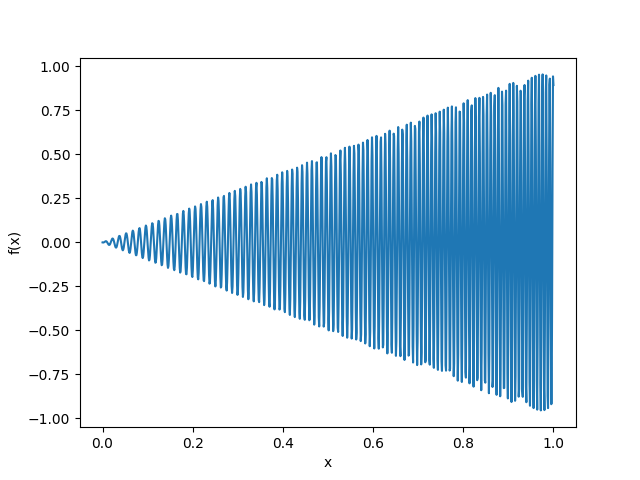
\includegraphics[width=\linewidth]{media/f.png}
        \caption*{$f(x) = x\sin(200 (x+1)^2)$}
    \end{minipage}
    \begin{minipage}[t]{0.32\linewidth}
        \centering
        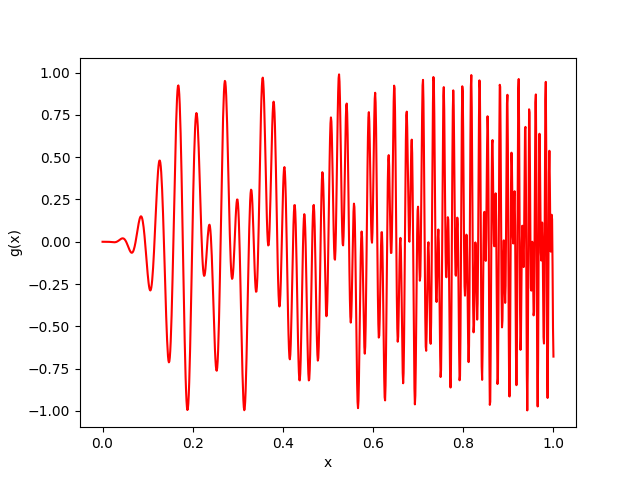
\includegraphics[width=\linewidth]{media/g.png}
        \caption*{$g(x)=250x^3 \cos(150x)$}
    \end{minipage}
    \begin{minipage}[t]{0.32\linewidth}
        \centering
        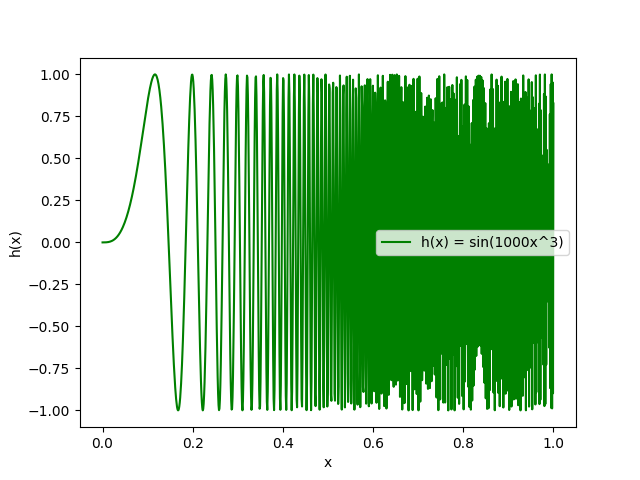
\includegraphics[width=\linewidth]{media/h.png}
        \caption*{$h(x)=\sin(1000x^3)$}
    \end{minipage}
\end{adjustwidth}
    \caption{The three high oscilatory functions that we will use to represent objective tensors}
\end{figure}

We will pick each function and we will evaluate it over the interval $[0,1]$ by uniformly picking $N$ samples. We will construct the
vectors 
$$v_F = \left( f\left(\frac{i}{N}\right) \right)_{i=1}^N \qquad
v_G = \left( g\left(\frac{i}{N}\right) \right)_{i=1}^N \qquad
v_H = \left( h\left(\frac{i}{N}\right) \right)_{i=1}^N \qquad$$
And we will reshape this tensors onto a shape $N_1 \times \cdots \times N_n$ such that $\prod_{i=1}^n N_i = N$
$$
T_F = \reshape(v_F, (1), (N_1, \dots, N_n)) \qquad
T_G = \reshape(v_G, (1), (N_1, \dots, N_n))$$
$$T_H = \reshape(v_H, (1), (N_1, \dots, N_n))$$

We tested $6$ different tensor network structures. The graphs $G_1, \dots, G_6$ are as defined in \ref{fig:ap-graphs}
the ranks of each graph are $R_1 = (5, 5, 5)$, $R_2 = (10, 10, 10)$, $R_3 = (7,7,7,7,7)$, $R_4 = (7,7,7,7,7,7)$,
$R_5 = (12, 12, 12 ,12)$ and $R_6 = (3,3,3,3,3,3,3,3,3,3,3,3,3,3,3)$.

The results of the experiment are shown in \figref{fig:ap-table-backprop}.

\begin{figure}[H]
    \begin{minipage}[t]{0.32\linewidth}
        \centering
        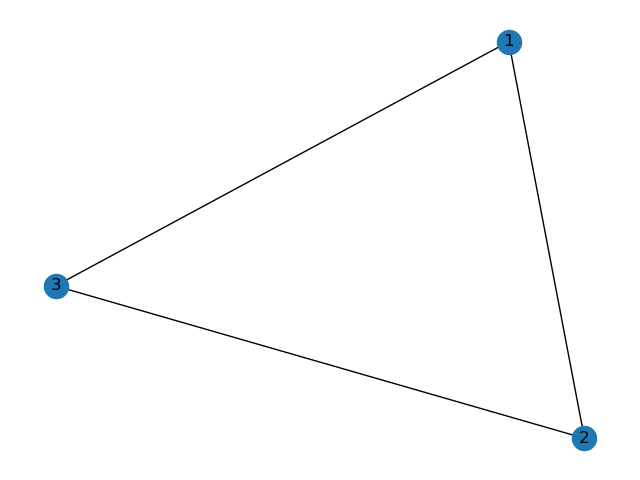
\includegraphics[width=\linewidth]{media/graph-backprop-1.png}
        \caption*{$G_1$}
    \end{minipage}
    \begin{minipage}[t]{0.32\linewidth}
        \centering
        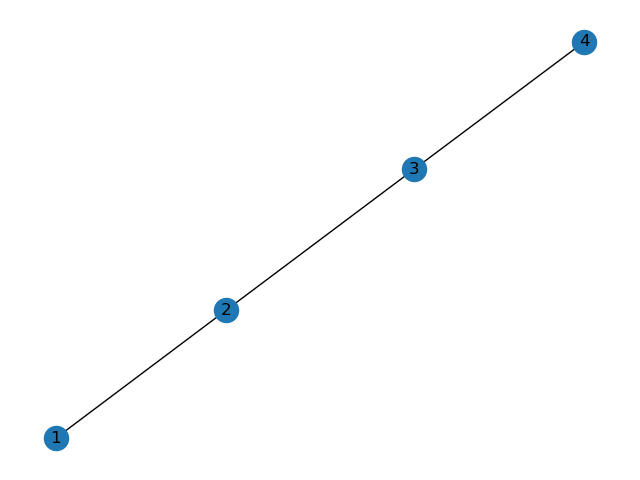
\includegraphics[width=\linewidth]{media/graph-backprop-2.png}
        \caption*{$G_2$}
    \end{minipage}
    \begin{minipage}[t]{0.32\linewidth}
        \centering
        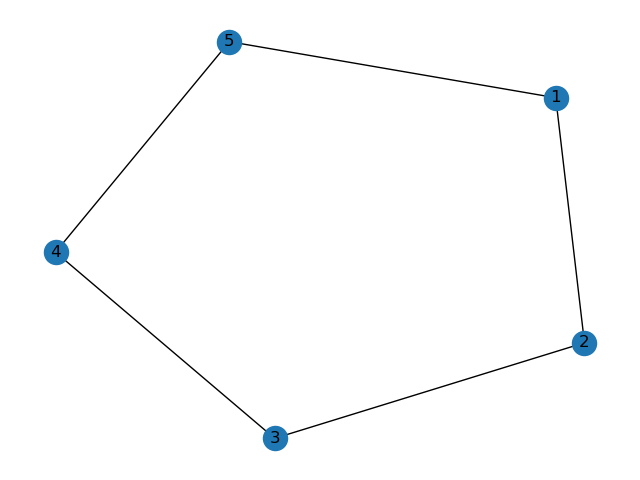
\includegraphics[width=\linewidth]{media/graph-backprop-3.png}
        \caption*{$G_3$}
    \end{minipage}

   \begin{minipage}[t]{0.32\linewidth}
        \centering
        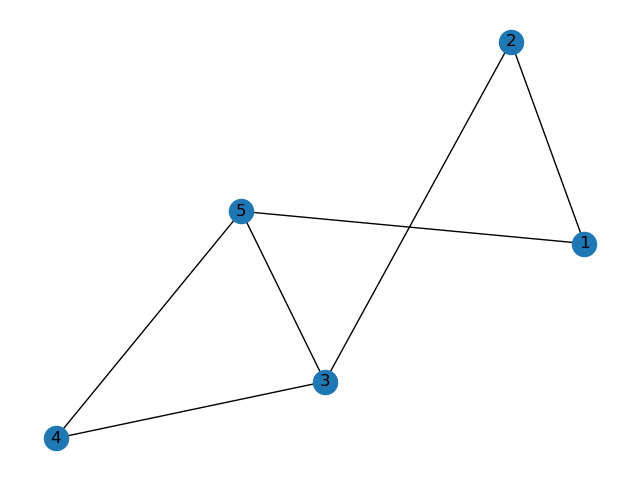
\includegraphics[width=\linewidth]{media/graph-backprop-4.png}
        \caption*{$G_4$}
    \end{minipage}
    \begin{minipage}[t]{0.32\linewidth}
        \centering
        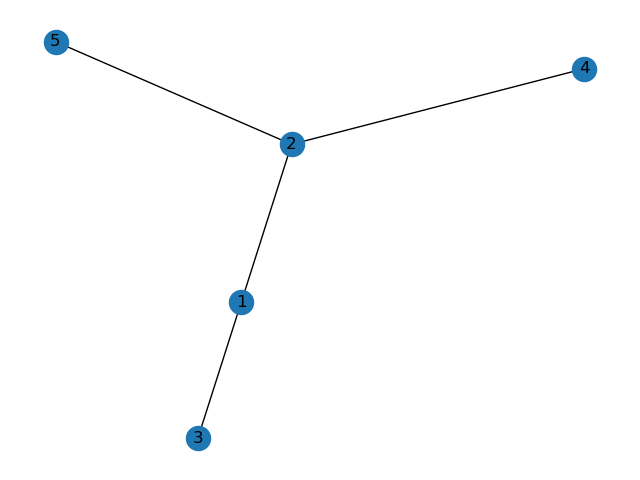
\includegraphics[width=\linewidth]{media/graph-backprop-5.png}
        \caption*{$G_5$}
    \end{minipage}
    \begin{minipage}[t]{0.32\linewidth}
        \centering
        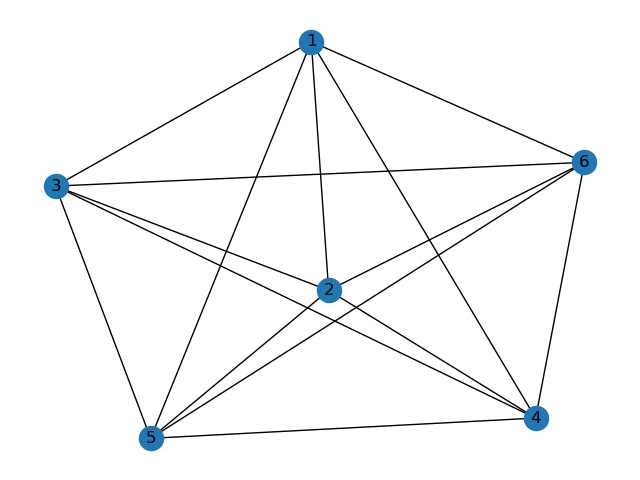
\includegraphics[width=\linewidth]{media/graph-backprop-6.png}
        \caption*{$G_6$}
    \end{minipage}
    \caption{The graphs $G_1, \dots, G_6$ used for each test. Source: own elaboration.}
    \label{fig:ap-graphs}
\end{figure}

\begin{figure}
    \centering
\renewcommand{\arraystretch}{1.25}
\begin{tabular}{lllllll}
\hline
          &          & Time & CR & $T_F$ Rel. Error & $T_G$ Rel. Error & $T_H$ Rel. Error\\ \hline
    $(G_1, R_1)$ & TN-ALS   & 5s & $1.34$ & $\mathbf{6.9456 \times 10^{-3}}$            & $\mathbf{1.0652 \times 10^{-2}}$            & $7.9986 \times 10^{-2}$           \\
                 & Backprop &  & & $2.1491 \times 10^{-2}$                     & $5.0026 \times 10^{-2}$                     & $\mathbf{6.1857 \times 10^{-2}}$          \\ \hline
    $(G_2, R_2)$ & TN-ALS   & 5s & $4.55$ & $\mathbf{1.9582 \times 10^{-4}}$            & $\mathbf{8.9858 \times 10^{-5}}$        & $\mathbf{0.113449}$           \\
                 & Backprop & &  & $2.8724 \times 10^{-2}$                     & $2.8724 \times 10^{-2}$                     & $0.115987$           \\ \hline
    $(G_3, R_3)$ & TN-ALS   & 5s & $40.82$ & $\mathbf{4.7541 \times 10^{-3}}$            & $\mathbf{9.5917 \times 10^{-3}}$        & $\mathbf{4.4717 \times 10^{-2}}$           \\
                 & Backprop & & & $3.1899 \times 10^{-2}$                     & $4.9388 \times 10^{-2}$                     & $4.5730 \times 10^{-2}$           \\ \hline
    $(G_4, R_4)$ & TN-ALS   & 5s & $12$ & $\mathbf{7.1427 \times 10^{-4}}$            & $\mathbf{1.6699 \times 10^{-3}}$        & $\mathbf{1.1705 \times 10^{-2}}$           \\
                 & Backprop & & & $8.3855 \times 10^{-2}$                     & $8.7846 \times 10^{-2}$                     & $4.5468 \times 10^{-2}$           \\ \hline
    $(G_5, R_5)$ & TN-ALS   & 5s & $5.24$ & $\mathbf{4.5774 \times 10^{-2}}$            & $\mathbf{6.8181 \times 10^{-2}}$        & $0.203061$           \\
                 & Backprop & & & $5.3277 \times 10^{-2}$                     & $7.4776 \times 10^{-2}$                     & $\mathbf{0.200155}$           \\ \hline
    $(G_6, R_6)$ & TN-ALS   & 10s & $68.59$ & $\mathbf{1.9251 \times 10^{-3}}$           & $\mathbf{2.4820 \times 10^{-3}}$        & $\mathbf{2.0864 \times 10^{-2}}$           \\
                 & Backprop & & & $0.880255$                                 & $0.751659$                                  & $0.572296$         \\ \hline
\end{tabular}

\caption{Relative error obtained by running the TN-ALS algorithm and the backpropagation algorithm for approximating
    the tensors $T_F, T_G$ and $T_H$ fot the same fixed amount of time. The CR column denotes the compression ratio of each structure.
In each test the result with less relative error is marked in bold test. Source: own elaboration}
\label{fig:ap-table-backprop}
\end{figure}

\section{Structure search and image compression}

On the next experiment we evaluated the performance of the \gls{TnALE} algorithm and the optimal structures that it finds. The objective tensor
that we will approximate will be the intensity values of the pixels of an image.

An RGB image is a set of $n \times m$ pixels. Each pixel contains
three channels (red, green and blue) in which a color is represented. 
For simplicity, in this experiment we will only encode grayscale images since grayscale images
only need to store the intensity value of each pixel. Therefore, we can encode a channel as
as a tensor $T \in \mathbb{R}^{n \times m}$ with each of its values
being on the interval $[0,1] \subset \mathbb{R}$.

First, we could make the order of the tensor $T$ higher by reshaping accordingly the divisors of $n$ or $m$. For example,
if we have a $128 \times 128$ image, we could reshape $T$ as tensor of $\mathbb{R}^{8 \times 8 \times 4 \times 8 \times 8 }$

Then reshaping, for each channel we could pick a graph $G^{(0)}$ with the number of nodes being equal as the order of the tensors. Following our example,
$G$ should have $6$ nodes. We can also pick some initial ranks $R^{(0)} = (R_1, \dots, R_c)$. Then we can apply the ALS algorithm for
finding some cores $\mathcal{G}_1, \dots, \mathcal{G}_6$ that once contracted following $G^{(0)}$ will yield to a good approximation
of $T$

Now, we apply the \gls{TnALE} algorithm for finding if there is a more optimal structure than $(G^{(0)}, R^{(0)})$. Once we found a good
structure candidate $(G^*, R^*)$ we then perform the TnALS algorithm using this structure.

Then, to recover the channel back we contract all the core tensors and then undo the reshape operation to recover the matrix that
encodes the image channel. Following our example, we would reshape the tensor $T \in \mathbb{R}^{ 8 \times 8 \times 4 \times 8 \times 8}$
obtained by contracting the cores found by TnALS into a matrix of $\mathbb{R}^{128 \times 128}$.

The main objective of this experiment is to demonstrate the compression capabilities of the optimal structure of the \gls{TnALE} algorithm by
doing image compression. For measuring the error we used the relative error of the objective tensor representing the grayscale channel
of the original tensor respect to the tensor that the contraction of the cores yields.

In this experiment we compressed the image \verb|files/fruits.png| grayscaled and resized as a $128 \times 128$ image.
We fixed $5$ initial pairs of initial structures $(G^{(1)}, R^{(1)}), \dots, (G^{(5)}, R^{(5)})$.
For each structure we first computed the core tensors using the TnALS algorithms directly, and then
we made the \gls{TnALE} algorithm find a better structure by varying $\lambda \in \{0.25, 0.5, 1, 2, 4, 8, 12\}$. We use the
\gls{TnALE} algorithm two times: first, we make broad search by doing $3$ iterations of it with radius $5$ that are able to modify
the topology of the original graph $G_0$. We made that if the algorithm decided to add an edge, it will try doing so by putting initial
ranks $\{1, 2, 5\}$. Then, we do again the \gls{TnALE} algorithm with $3$ iterations with radius $2$ and we let $G$ fixed so that
the structure can be relaxed to adjust its ranks. On both \gls{TnALE} calls we use the
\gls{TnALS} algorithm with $5$ iterations applying the Tikhonov factor for faster computation and
for getting the minimum relative error by 
picking the minimum value of the relative error in these $5$ iterations.
After we have found an optimal structure, we finally perform the TnALS algorithm with $200$ iterations. 

The starting graphs $G^{(1)},\dots , G^{(5)}$ that we have picked can be seen in the first row of \figref{fig:ap-lots-of-graphs}.
We will also describe explicitly the order of the starting edges $E^{(1)}, \dots, E^{(5)}$ and the starting ranks $R^{(1)}, \dots, R^{(5)}$: 

\begin{itemize}
    \item $E^{(1)} = ((1,2), (2, 3), (3, 4), (4, 5))$ \\ 
        $R^{(1)} = (8,8,8,8)$
    \item $E^{(2)} = ((1,2), (2, 3), (3, 4), (4, 5), (5, 1))$ \\
        $R^{(2)} = (8,8,8,8,8)$
    \item $E^{(3)} = ((1,2), (2, 3), (3, 4), (4, 5), (5, 1), (3, 5), (1, 4))$ \\
        $R^{(3)} = (6,6,6,6,6,6,6)$
    \item $E^{(4)} = ((1,2), (2, 3), (3, 4), (4, 5), (5, 1), (1, 4), (5, 2), (3, 5))$ \\
        $R^{(4)} = (4,4,4,4, 4,4,4,4)$
    \item $E^{(5)} = ((1,2), (2, 3), (3, 4), (4, 5), (5, 1), (5, 2), (5, 3), (4, 1), (4, 2), (3, 1))$ \\
        $R^{(5)} = (3,3,4,3,3,4,3,3,4,3)$
\end{itemize}

The final ranks that produced each execution can be found inside the text files of the folder \verb|files/img-compression/|

\begin{figure}[h]
\begin{adjustwidth}{-30pt}{-30pt}
    \centering

\begin{tabular}{lllllll}
\hline
                     &                  & CR     & Rel. Error & TN-ALS & TN-ALE First Pass & TN-ALE Second Pass \\ \hline
$(G^{(1)}, R^{(1)})$ & Original         & 11.63  & 0.13159    & 3.08s  &                   &                    \\
                     & $\lambda = 0.25$ & 455.11 & 0.19703    & 3.08s  & 4.84s             & 0.23s              \\
                     & $\lambda = 0.5$  & 105.02 & 0.16981    & 1.95s  & 6.65s             & 1.56s              \\
                     & $\lambda = 1$    & 34.13  & 0.13397    & 2.45s  & 7.49s             & 2.97s              \\
                     & $\lambda = 2$    & 23.81  & 0.12605    & 2.40s  & 9.81s             & 2.99s              \\
                     & $\lambda = 4$    & 10.06  & 0.10416    & 3.24s  & 22.85s            & 4.66s              \\
                     & $\lambda = 8$    & 4.61   & 0.07901    & 6.43s  & 55.36s            & 10.77s             \\
                     & $\lambda = 12$   & 2.16   & 0.05304    & 14.10s & 122.91s           & 20.13s             \\ \hline
$(G^{(2)}, R^{(2)})$ & Original         & 7.11   & 0.09592    & 3.56s  &                   &                    \\
                     & $\lambda = 0.25$ & 455.11 & 0.19703    & 1.39s  & 5.65s             & 0.64s              \\
                     & $\lambda = 0.5$  & 50.56  & 0.14933    & 2.09s  & 6.07s             & 2.92s              \\
                     & $\lambda = 1$    & 32.51  & 0.13736    & 2.29s  & 6.68s             & 3.63s              \\
                     & $\lambda = 2$    & 18.62  & 0.12109    & 2.77s  & 8.55s             & 4.22s              \\
                     & $\lambda = 4$    & 9.62   & 0.10570    & 3.45s  & 17.28s            & 4.98s              \\
                     & $\lambda = 8$    & 3.52   & 0.07178    & 8.65s  & 190.7s            & 11.59s             \\
                     & $\lambda = 12$   & 2.12   & 0.05678    & 15.39s & 143.14s           & 29.29s             \\ \hline
$(G^{(3)}, R^{(3)})$ & Original         & 2.58   & 0.06481    & 9.81s  &                   &                    \\
                     & $\lambda = 0.25$ & 240.94 & 0.18556    & 1.81s  & 6.55s             & 3.20s              \\
                     & $\lambda = 0.5$  & 102.4  & 0.16595    & 2.15s  & 6.51s             & 2.44s              \\
                     & $\lambda = 1$    & 47.08  & 0.14801    & 2.40s  & 8.67s             & 4.29s              \\
                     & $\lambda = 2$    & 18.12  & 0.12340    & 2.76s  & 17.66s            & 5.79s              \\
                     & $\lambda = 4$    & 12.41  & 0.11887    & 3.18s  & 15.78s            & 5.15s              \\
                     & $\lambda = 8$    & 3.53   & 0.07238    & 10.19s & 61.14s            & 22.02s             \\
                     & $\lambda = 12$   & 2.11   & 0.04997    & 21.57s & 284.93s           & 29.51s             \\ \hline
$(G^{(4)}, R^{(4)})$ & Original         & 4.26   & 0.08985    & 5.46s  &                   &                    \\
                     & $\lambda = 0.25$ & 113.78 & 0.17616    & 2.03s  & 11.63s            & 2.39s              \\
                     & $\lambda = 0.5$  & 89.04  & 0.16479    & 1.92s  & 11.59s            & 2.62s              \\
                     & $\lambda = 1$    & 40.96  & 0.14096    & 2.26s  & 11.62s            & 2.78s              \\
                     & $\lambda = 2$    & 24.38  & 0.13249    & 2.45s  & 11.99s            & 3.11s              \\
                     & $\lambda = 4$    & 11.91  & 0.11154    & 3.11s  & 12.73s            & 6.07s              \\
                     & $\lambda = 8$    & 3.28   & 0.06162    & 6.84s  & 28.71s            & 13.91s             \\
                     & $\lambda = 12$   & 2.75   & 0.06293    & 8.81s  & 70.02s            & 17.61s             \\ \hline
$(G^{(5)}, R^{(5)})$ & Original         & 3.92   & 0.07800    & 6s     &                   &                    \\
                     & $\lambda = 0.25$ & 204.8  & 0.18553    & 1.95s  & 13.86s            & 3.58s              \\
                     & $\lambda = 0.5$  & 70.62  & 0.15677    & 2.14s  & 13.89s            & 3.97s              \\
                     & $\lambda = 1$    & 39.38  & 0.14342    & 2.38s  & 13.96s            & 4.92s              \\
                     & $\lambda = 2$    & 16.38  & 0.12128    & 2.92s  & 14.62s            & 5.46s              \\
                     & $\lambda = 4$    & 9.57   & 0.10488    & 3.39s  & 14.78s            & 6.38s              \\
                     & $\lambda = 8$    & 6.82   & 0.09066    & 3.89s  & 21.7s             & 12.79s             \\
                     & $\lambda = 12$   & 2.33   & 0.05597    & 10.43s & 58.08s            & 22.48s            
\end{tabular}

\end{adjustwidth}

\caption{Table containing the results of the TnALE evaluation compressing the pepper.png image. Source: own elaboration}
\label{fig:ap-lots-of-numbers}
\end{figure}

% Figura molt gran
\begin{figure}[h]

\begin{adjustwidth}{-3cm}{-3cm}

    \centering
    \def\arraystretch{1.15}
\begin{tabular}{>{\centering\arraybackslash}m{1.5cm} m{2.5cm} m{2.5cm} m{2.5cm} m{2.5cm} m{2.5cm}}
        & \centering $G^{(1)}$ & \centering $G^{(2)}$ & \centering $G^{(3)}$ & \centering $G^{(4)}$ & \centering $G^{(5)}$ & \\ \hline
        Orig. &
        \rule{0pt}{0.01cm} 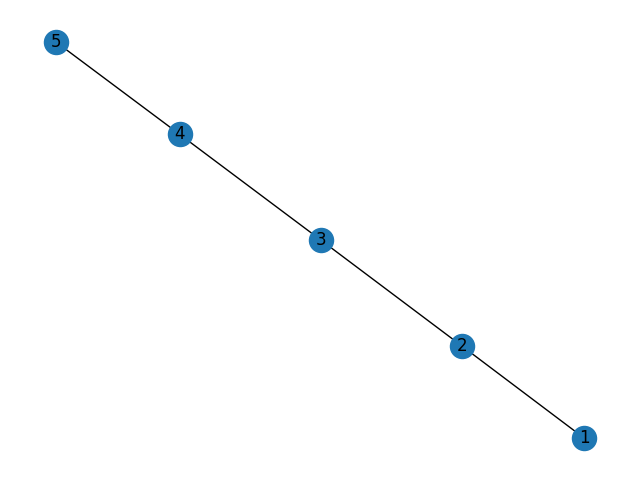
\includegraphics[width=\linewidth]{media/tnale/graph-1.png} \rule{0pt}{0.01cm} & 
        \rule{0pt}{0.01cm} 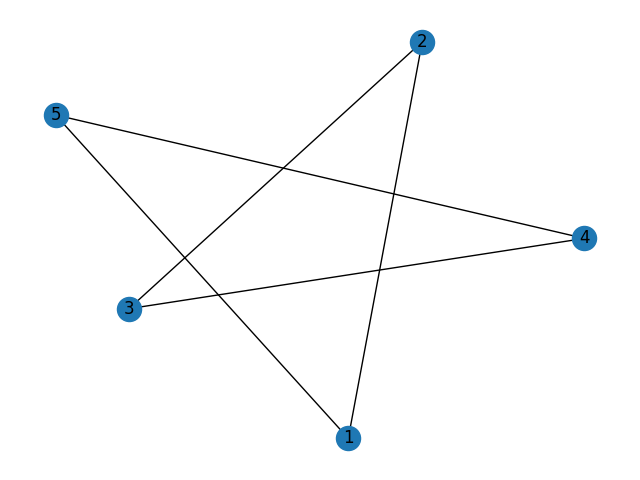
\includegraphics[width=\linewidth]{media/tnale/graph-2.png} \rule{0pt}{0.01cm} &
        \rule{0pt}{0.01cm} 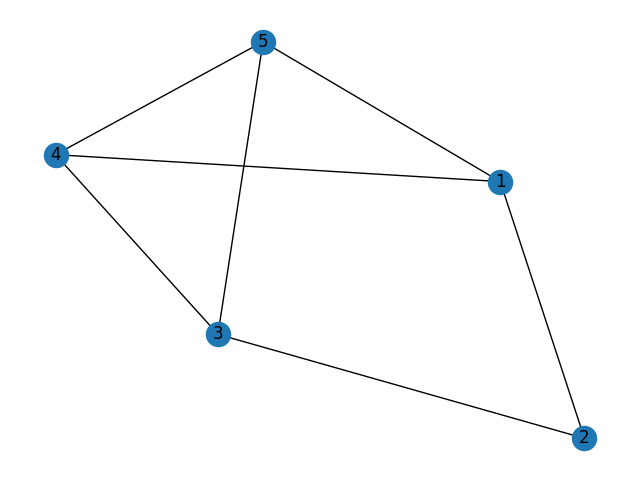
\includegraphics[width=\linewidth]{media/tnale/graph-3.png} \rule{0pt}{0.01cm} & 
        \rule{0pt}{0.01cm} 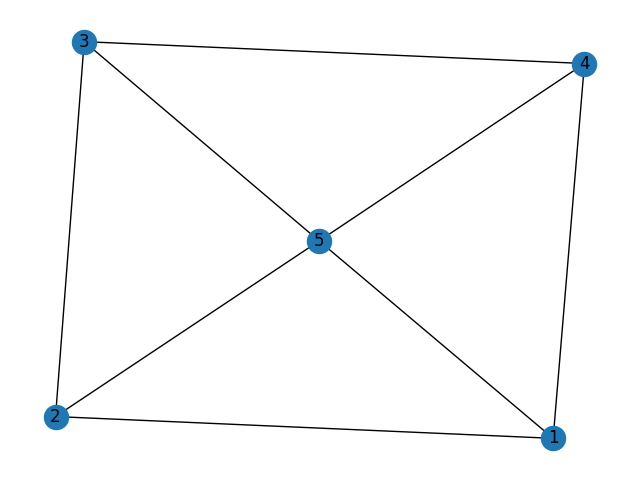
\includegraphics[width=\linewidth]{media/tnale/graph-4.png} \rule{0pt}{0.01cm} &
        \rule{0pt}{0.01cm} 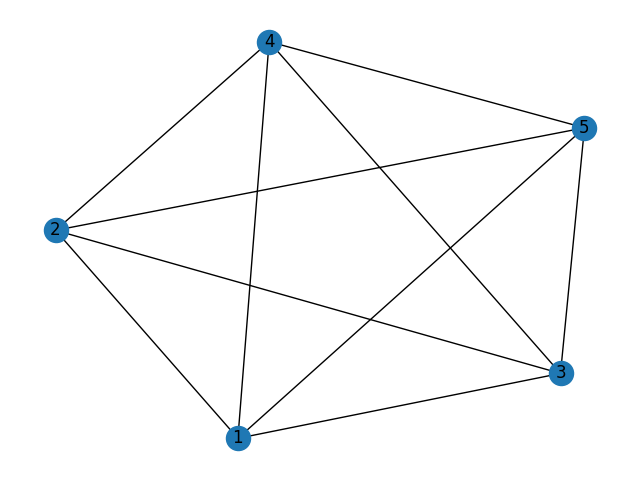
\includegraphics[width=\linewidth]{media/tnale/graph-5.png} \rule{0pt}{0.01cm} \\ \hline
        $\lambda = 0.25$ &
        \rule{0pt}{0.01cm} 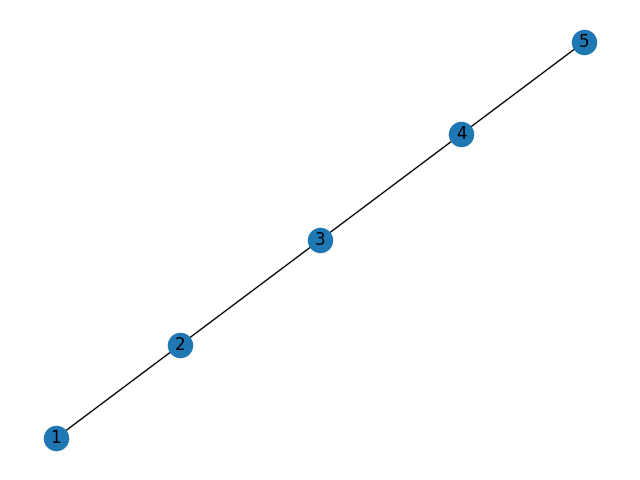
\includegraphics[width=\linewidth]{media/tnale/graph-1-tnale-0.25.png} \rule{0pt}{0.01cm} &
        \rule{0pt}{0.01cm} 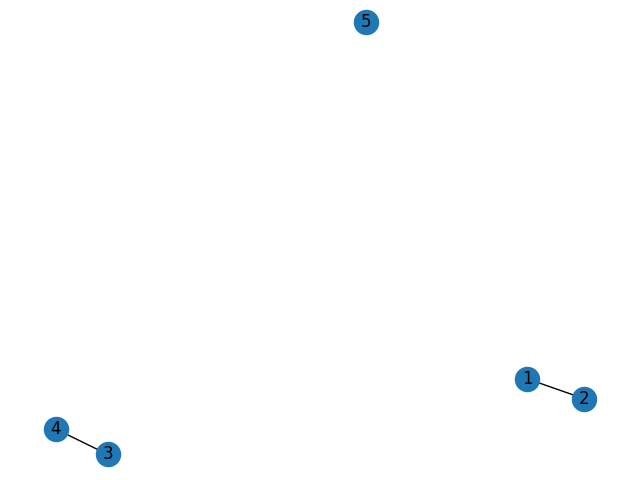
\includegraphics[width=\linewidth]{media/tnale/graph-2-tnale-0.25.png} \rule{0pt}{0.01cm} &
        \rule{0pt}{0.01cm} 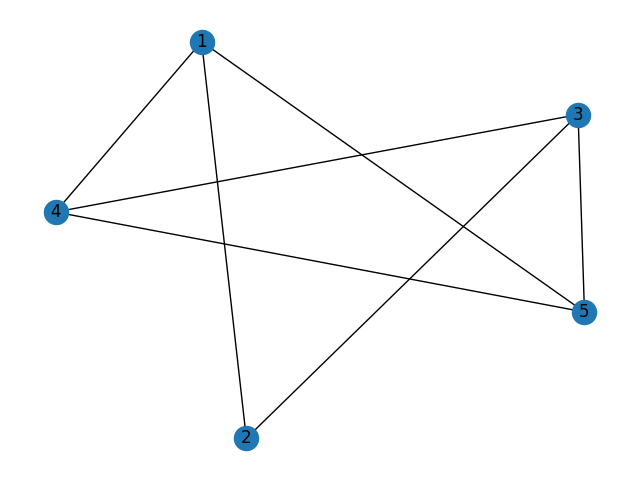
\includegraphics[width=\linewidth]{media/tnale/graph-3-tnale-0.25.png} \rule{0pt}{0.01cm} & 
        \rule{0pt}{0.01cm} 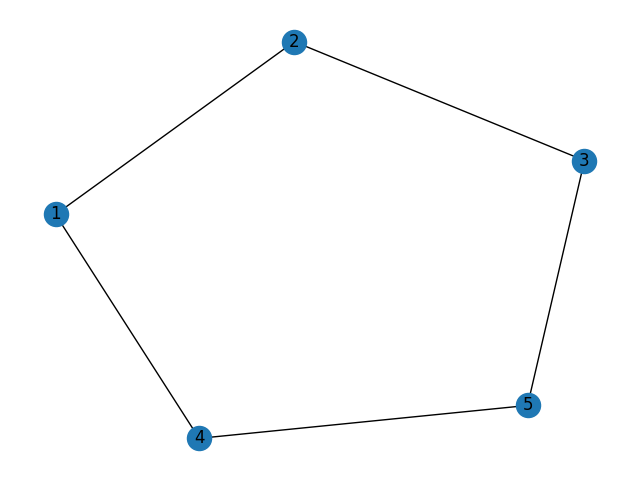
\includegraphics[width=\linewidth]{media/tnale/graph-4-tnale-0.25.png} \rule{0pt}{0.01cm} &
        \rule{0pt}{0.01cm} 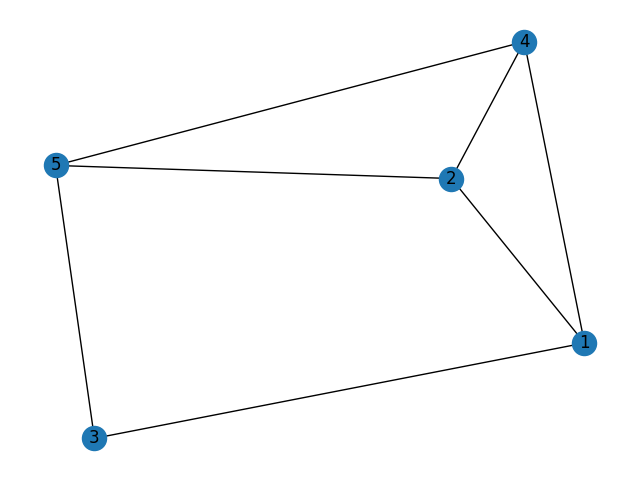
\includegraphics[width=\linewidth]{media/tnale/graph-5-tnale-0.25.png} \rule{0pt}{0.01cm} \\ \hline
        $\lambda = 0.5$ &
        \rule{0pt}{0.01cm} 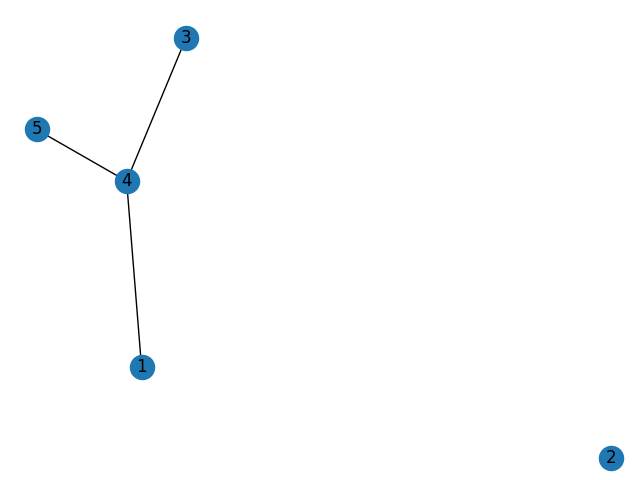
\includegraphics[width=\linewidth]{media/tnale/graph-1-tnale-0.5.png} \rule{0pt}{0.01cm}&
        \rule{0pt}{0.01cm} 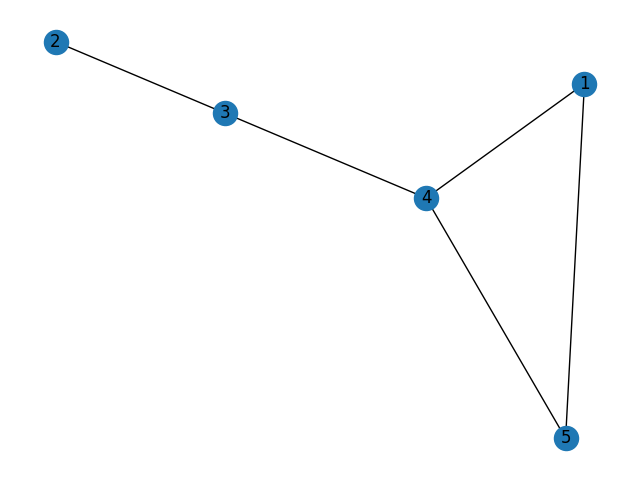
\includegraphics[width=\linewidth]{media/tnale/graph-2-tnale-0.5.png} \rule{0pt}{0.01cm}&
        \rule{0pt}{0.01cm} 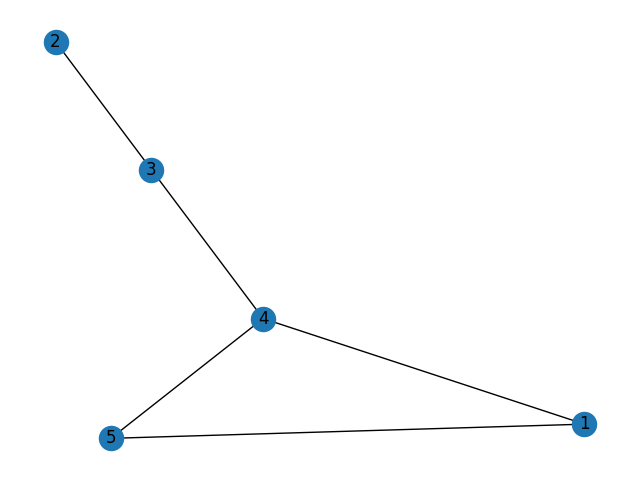
\includegraphics[width=\linewidth]{media/tnale/graph-3-tnale-0.5.png} \rule{0pt}{0.01cm}& 
        \rule{0pt}{0.01cm} 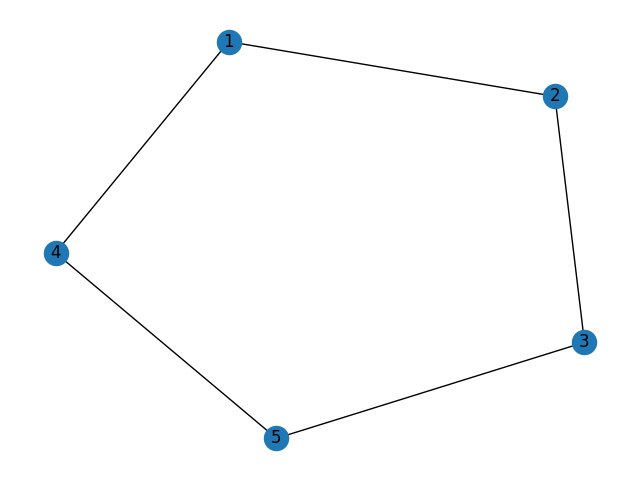
\includegraphics[width=\linewidth]{media/tnale/graph-4-tnale-0.5.png} \rule{0pt}{0.01cm}&
        \rule{0pt}{0.01cm} 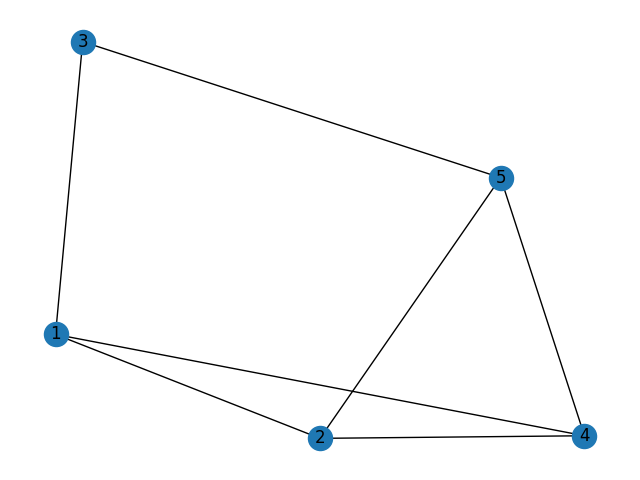
\includegraphics[width=\linewidth]{media/tnale/graph-5-tnale-0.5.png} \rule{0pt}{0.01cm}\\ \hline
        $\lambda = 1$ &
        \rule{0pt}{0.01cm} 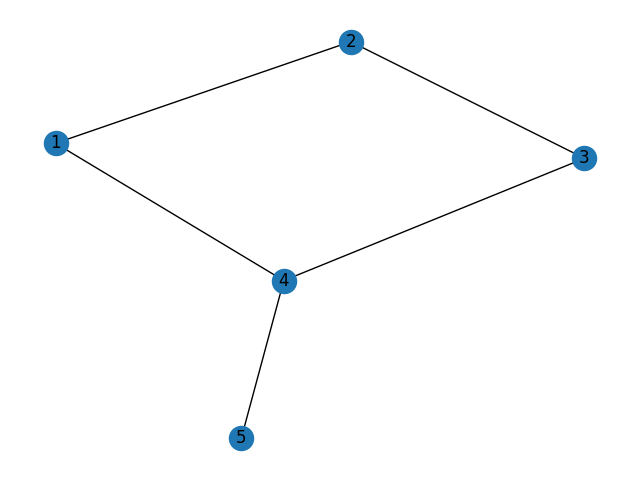
\includegraphics[width=\linewidth]{media/tnale/graph-1-tnale-1.png} \rule{0pt}{0.01cm}&
        \rule{0pt}{0.01cm} 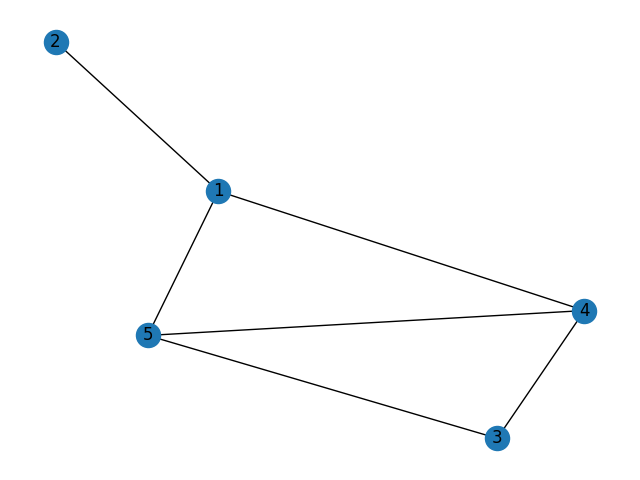
\includegraphics[width=\linewidth]{media/tnale/graph-2-tnale-1.png} \rule{0pt}{0.01cm}&
        \rule{0pt}{0.01cm} 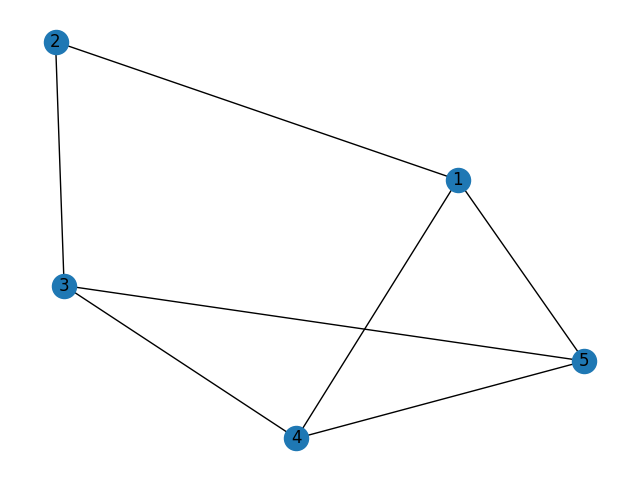
\includegraphics[width=\linewidth]{media/tnale/graph-3-tnale-1.png} \rule{0pt}{0.01cm}& 
        \rule{0pt}{0.01cm} 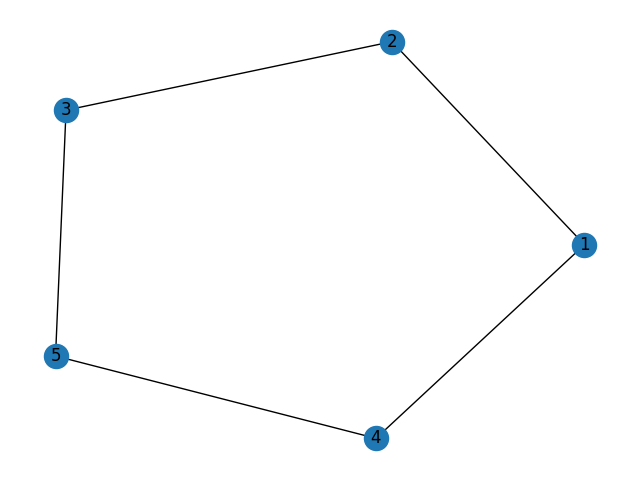
\includegraphics[width=\linewidth]{media/tnale/graph-4-tnale-1.png} \rule{0pt}{0.01cm}&
        \rule{0pt}{0.01cm} 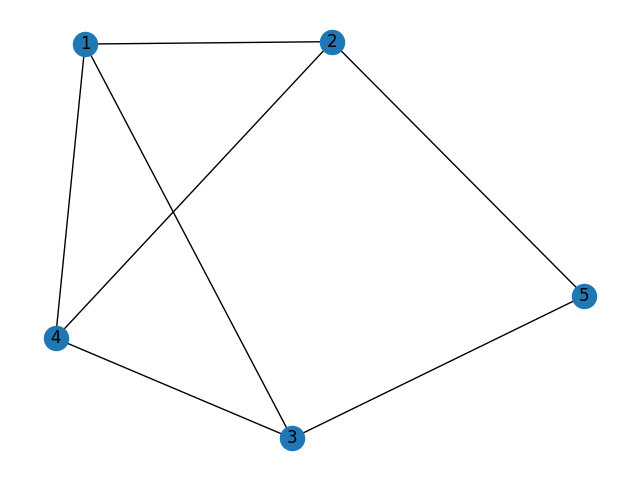
\includegraphics[width=\linewidth]{media/tnale/graph-5-tnale-1.png} \rule{0pt}{0.01cm}\\ \hline
        $\lambda = 2$ &
        \rule{0pt}{0.01cm} 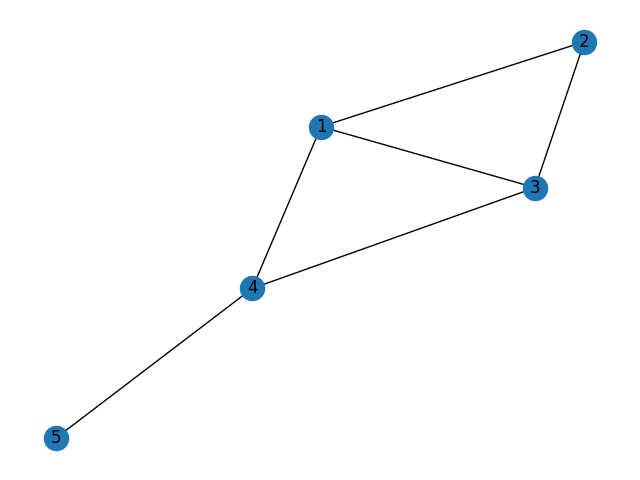
\includegraphics[width=\linewidth]{media/tnale/graph-1-tnale-2.png} \rule{0pt}{0.01cm}&
        \rule{0pt}{0.01cm} 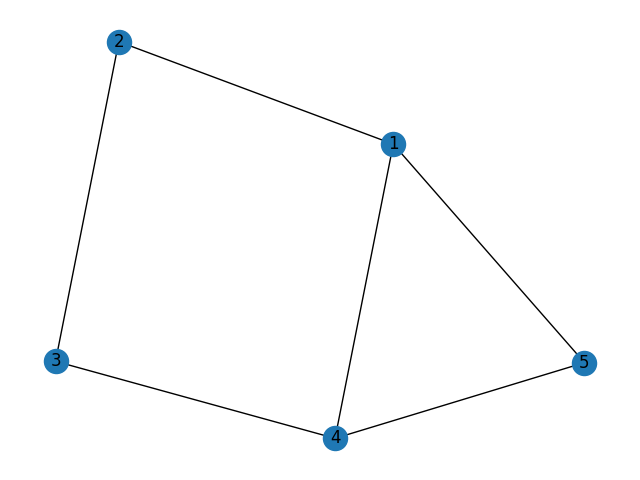
\includegraphics[width=\linewidth]{media/tnale/graph-2-tnale-2.png} \rule{0pt}{0.01cm}&
        \rule{0pt}{0.01cm} 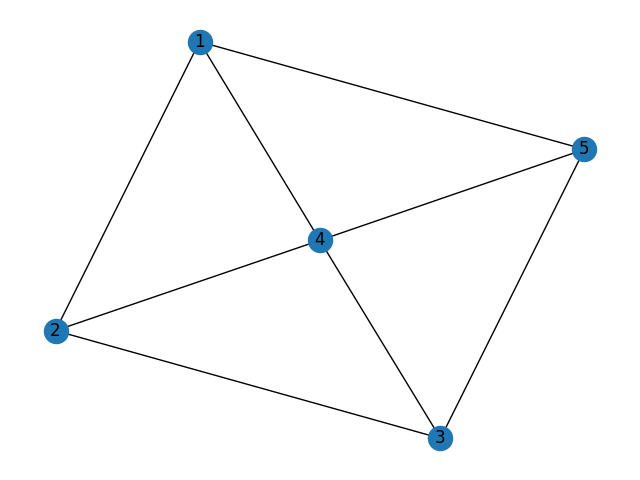
\includegraphics[width=\linewidth]{media/tnale/graph-3-tnale-2.png} \rule{0pt}{0.01cm}& 
        \rule{0pt}{0.01cm} 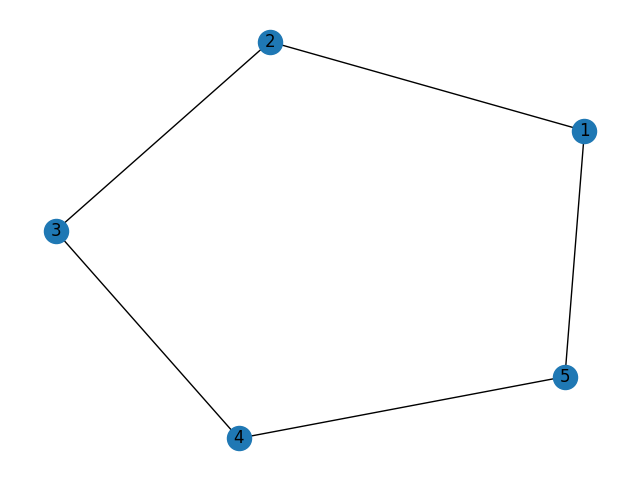
\includegraphics[width=\linewidth]{media/tnale/graph-4-tnale-2.png} \rule{0pt}{0.01cm}&
        \rule{0pt}{0.01cm} 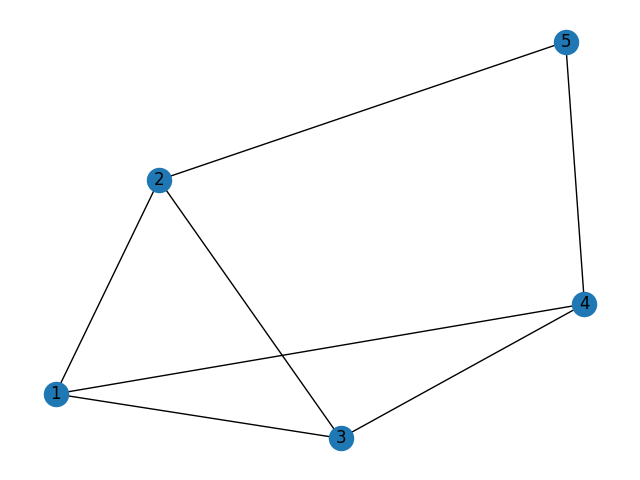
\includegraphics[width=\linewidth]{media/tnale/graph-5-tnale-2.png} \rule{0pt}{0.01cm}\\ \hline
        $\lambda = 4$ &
        \rule{0pt}{0.01cm} 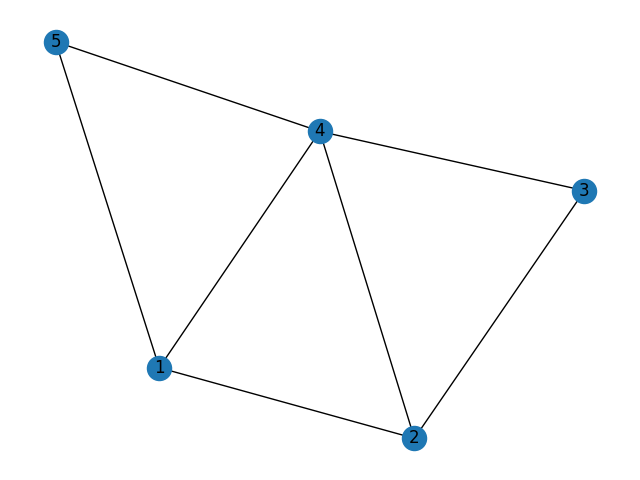
\includegraphics[width=\linewidth]{media/tnale/graph-1-tnale-4.png} \rule{0pt}{0.01cm}&
        \rule{0pt}{0.01cm} 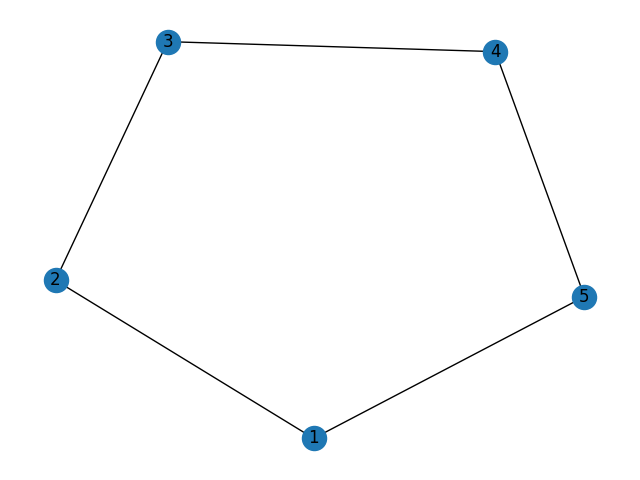
\includegraphics[width=\linewidth]{media/tnale/graph-2-tnale-4.png} \rule{0pt}{0.01cm}&
        \rule{0pt}{0.01cm} 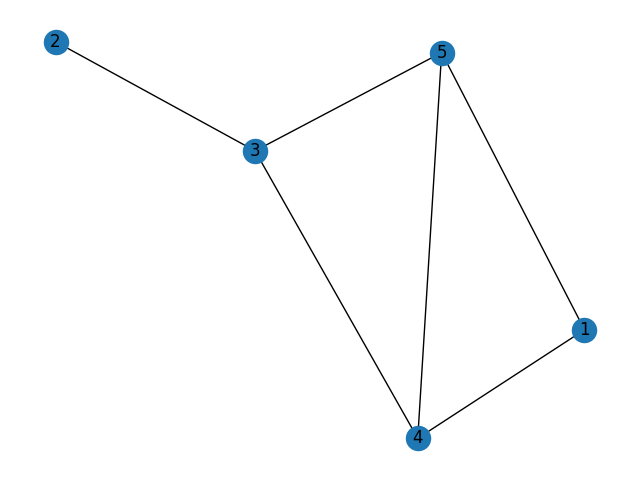
\includegraphics[width=\linewidth]{media/tnale/graph-3-tnale-4.png} \rule{0pt}{0.01cm}& 
        \rule{0pt}{0.01cm} 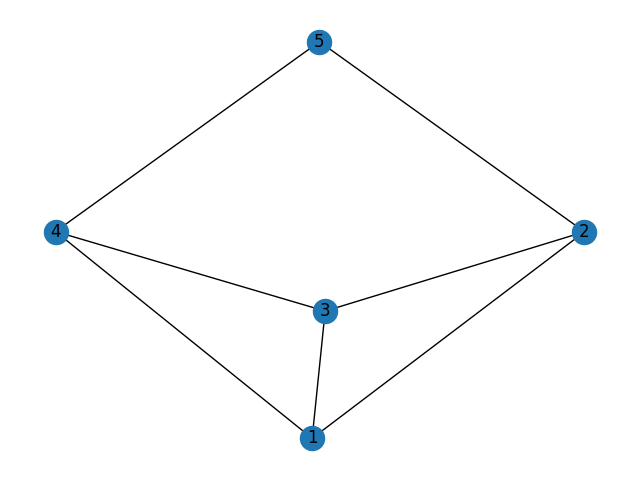
\includegraphics[width=\linewidth]{media/tnale/graph-4-tnale-4.png} \rule{0pt}{0.01cm}&
        \rule{0pt}{0.01cm} 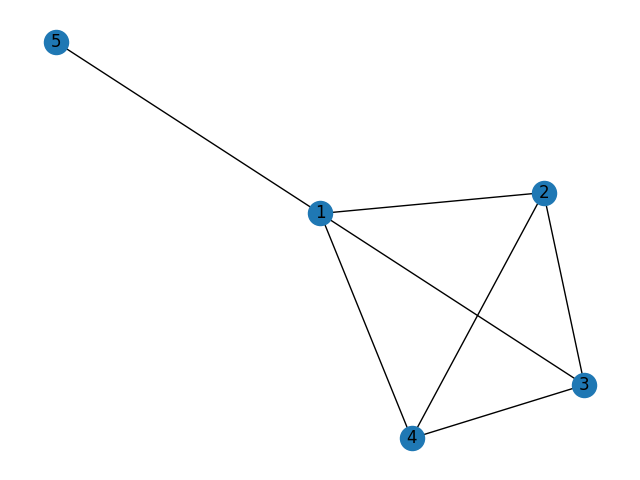
\includegraphics[width=\linewidth]{media/tnale/graph-5-tnale-4.png} \rule{0pt}{0.01cm}\\ \hline
        $\lambda = 8$ &
        \rule{0pt}{0.01cm} 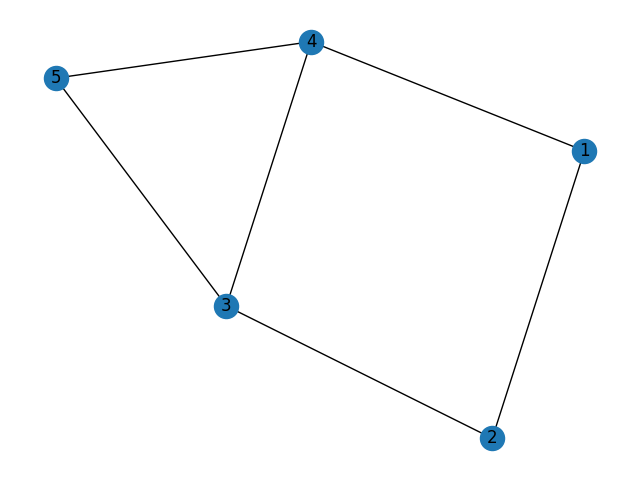
\includegraphics[width=\linewidth]{media/tnale/graph-1-tnale-8.png} \rule{0pt}{0.01cm}&
        \rule{0pt}{0.01cm} 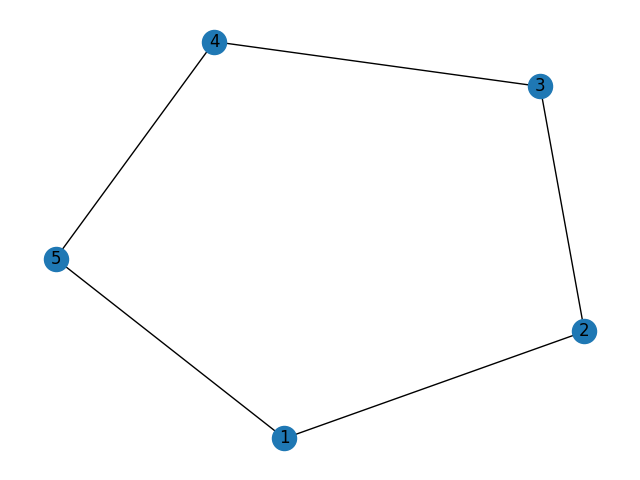
\includegraphics[width=\linewidth]{media/tnale/graph-2-tnale-8.png} \rule{0pt}{0.01cm}&
        \rule{0pt}{0.01cm} 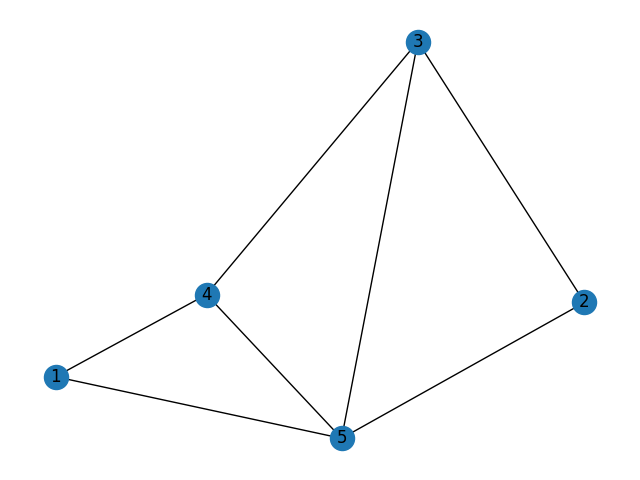
\includegraphics[width=\linewidth]{media/tnale/graph-3-tnale-8.png} \rule{0pt}{0.01cm}& 
        \rule{0pt}{0.01cm} 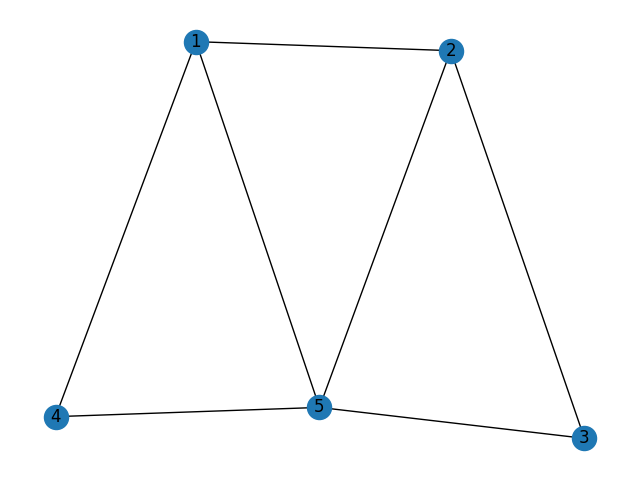
\includegraphics[width=\linewidth]{media/tnale/graph-4-tnale-8.png} \rule{0pt}{0.01cm}&
        \rule{0pt}{0.01cm} 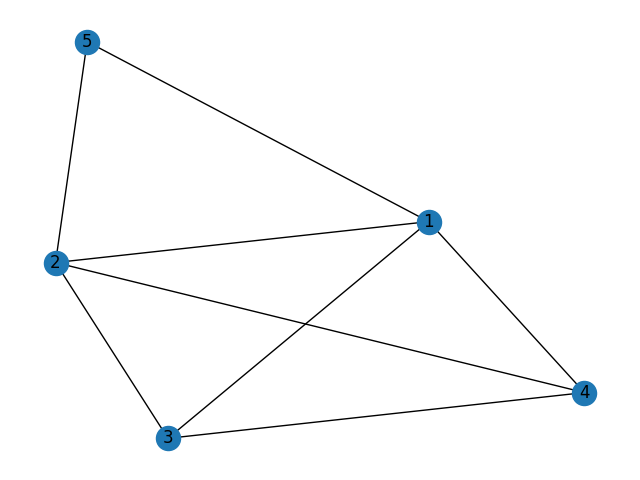
\includegraphics[width=\linewidth]{media/tnale/graph-5-tnale-8.png} \rule{0pt}{0.01cm}\\ \hline
        $\lambda = 12$ &
        \rule{0pt}{0.01cm} 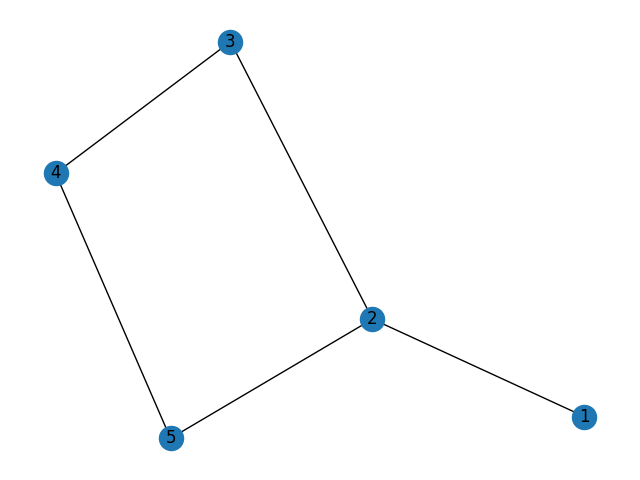
\includegraphics[width=\linewidth]{media/tnale/graph-1-tnale-12.png} \rule{0pt}{0.01cm}&
        \rule{0pt}{0.01cm} 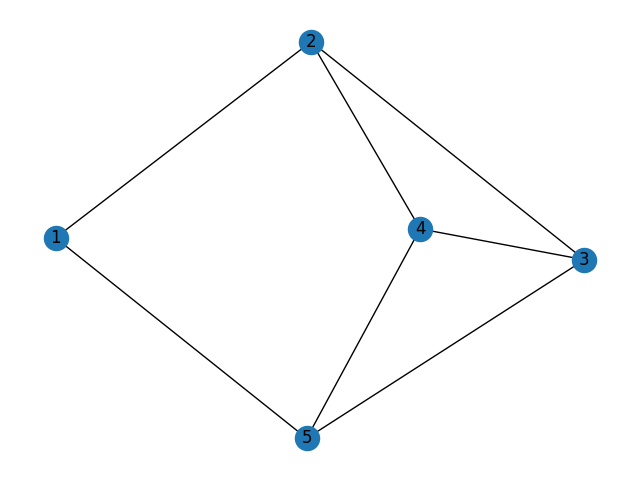
\includegraphics[width=\linewidth]{media/tnale/graph-2-tnale-12.png} \rule{0pt}{0.01cm}&
        \rule{0pt}{0.01cm} 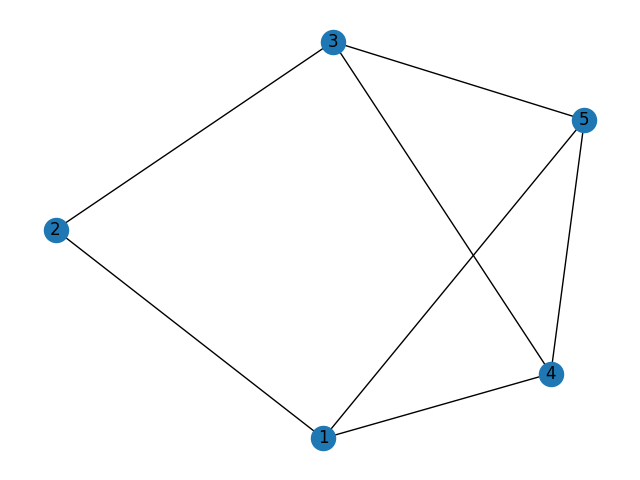
\includegraphics[width=\linewidth]{media/tnale/graph-3-tnale-12.png} \rule{0pt}{0.01cm}& 
        \rule{0pt}{0.01cm} \includegraphics[width=\linewidth]{media/tnale/graph-4-tnale-12.png} \rule{0pt}{0.01cm}&
        \rule{0pt}{0.01cm} \includegraphics[width=\linewidth]{media/tnale/graph-5-tnale-12.png} \rule{0pt}{0.01cm}\\
   \end{tabular}
\end{adjustwidth}

    \caption{The structures $G^*$ found by the TnALE algorithm. Source: own elaboration.}
    \label{fig:ap-lots-of-graphs}
\end{figure}




\begin{figure}[h]

\begin{adjustwidth}{-3cm}{-3cm}

    \centering
\begin{tabular}{>{\centering\arraybackslash}m{1.5cm} m{2.5cm} m{2.5cm} m{2.5cm} m{2.5cm} m{2.5cm}}
        & \centering $G^{(1)}$ & \centering $G^{(2)}$ & \centering $G^{(3)}$ & \centering $G^{(4)}$ & \centering $G^{(5)}$ & \\
        Orig. &
        \includegraphics[width=\linewidth]{media/tnale/AAAfruits-comp1.png} &
        \includegraphics[width=\linewidth]{media/tnale/AAAfruits-comp2.png} &
        \includegraphics[width=\linewidth]{media/tnale/AAAfruits-comp3.png} & 
        \includegraphics[width=\linewidth]{media/tnale/AAAfruits-comp4.png} &
        \includegraphics[width=\linewidth]{media/tnale/AAAfruits-comp5.png} \\
        
        $\lambda = 0.25$ &
        \includegraphics[width=\linewidth]{media/tnale/AAAfruits-comp1-ale-0.25.png} &
        \includegraphics[width=\linewidth]{media/tnale/AAAfruits-comp2-ale-0.25.png} &
        \includegraphics[width=\linewidth]{media/tnale/AAAfruits-comp3-ale-0.25.png} & 
        \includegraphics[width=\linewidth]{media/tnale/AAAfruits-comp4-ale-0.25.png} &
        \includegraphics[width=\linewidth]{media/tnale/AAAfruits-comp5-ale-0.25.png} \\

        $\lambda = 0.5$ &
        \includegraphics[width=\linewidth]{media/tnale/AAAfruits-comp1-ale-0.5.png} &
        \includegraphics[width=\linewidth]{media/tnale/AAAfruits-comp2-ale-0.5.png} &
        \includegraphics[width=\linewidth]{media/tnale/AAAfruits-comp3-ale-0.5.png} & 
        \includegraphics[width=\linewidth]{media/tnale/AAAfruits-comp4-ale-0.5.png} &
        \includegraphics[width=\linewidth]{media/tnale/AAAfruits-comp5-ale-0.5.png} \\

        $\lambda = 1$ &
        \includegraphics[width=\linewidth]{media/tnale/AAAfruits-comp1-ale-1.png} &
        \includegraphics[width=\linewidth]{media/tnale/AAAfruits-comp2-ale-1.png} &
        \includegraphics[width=\linewidth]{media/tnale/AAAfruits-comp3-ale-1.png} & 
        \includegraphics[width=\linewidth]{media/tnale/AAAfruits-comp4-ale-1.png} &
        \includegraphics[width=\linewidth]{media/tnale/AAAfruits-comp5-ale-1.png} \\
        
        $\lambda = 2$ &
        \includegraphics[width=\linewidth]{media/tnale/AAAfruits-comp1-ale-2.png} &
        \includegraphics[width=\linewidth]{media/tnale/AAAfruits-comp2-ale-2.png} &
        \includegraphics[width=\linewidth]{media/tnale/AAAfruits-comp3-ale-2.png} & 
        \includegraphics[width=\linewidth]{media/tnale/AAAfruits-comp4-ale-2.png} &
        \includegraphics[width=\linewidth]{media/tnale/AAAfruits-comp5-ale-2.png} \\
         
        $\lambda = 4$ &
        \includegraphics[width=\linewidth]{media/tnale/AAAfruits-comp1-ale-4.png} &
        \includegraphics[width=\linewidth]{media/tnale/AAAfruits-comp2-ale-4.png} &
        \includegraphics[width=\linewidth]{media/tnale/AAAfruits-comp3-ale-4.png} & 
        \includegraphics[width=\linewidth]{media/tnale/AAAfruits-comp4-ale-4.png} &
        \includegraphics[width=\linewidth]{media/tnale/AAAfruits-comp5-ale-4.png} \\
        
        $\lambda = 8$ &
        \includegraphics[width=\linewidth]{media/tnale/AAAfruits-comp1-ale-8.png} &
        \includegraphics[width=\linewidth]{media/tnale/AAAfruits-comp2-ale-8.png} &
        \includegraphics[width=\linewidth]{media/tnale/AAAfruits-comp3-ale-8.png} & 
        \includegraphics[width=\linewidth]{media/tnale/AAAfruits-comp4-ale-8.png} &
        \includegraphics[width=\linewidth]{media/tnale/AAAfruits-comp5-ale-8.png} \\
        
        $\lambda = 12$ &
        \includegraphics[width=\linewidth]{media/tnale/AAAfruits-comp1-ale-12.png} &
        \includegraphics[width=\linewidth]{media/tnale/AAAfruits-comp2-ale-12.png} &
        \includegraphics[width=\linewidth]{media/tnale/AAAfruits-comp3-ale-12.png} & 
        \includegraphics[width=\linewidth]{media/tnale/AAAfruits-comp4-ale-12.png} &
        \includegraphics[width=\linewidth]{media/tnale/AAAfruits-comp5-ale-12.png} \\
   \end{tabular}
\end{adjustwidth}


    \caption{The images produced by the contraction of the core tensors that the TnALS algorithm
    produced from the optimal structure that TnALE found for each value of $\lambda$ for each structure on
    \figref{fig:ap-lots-of-graphs}. Source: own elaboration.}
    \label{fig:ap-lots-of-fruits}
\end{figure}

% TODO: Treure conclusions d'això, però posar-ho al chapter 5

\section{Neural Network compression}

For this experiment we trained a classifier over the MNIST dataset. Using fully connected neural networks.
The MNIST dataset consists in total of two sets of images: one of 60,000 training images and another set of 10,000 testing images.
Each image has  


The architecture of the overall model can be seen in \ref{fig:neural-architecture}. Then, we compress each weight
layer using a defined tensor network structure. The input layer contains 784 neurons, the first hidden layer
contains 180 neurons, the second hidden layer 100 neurons and the output layer contains 10 neurons, which their output
determine the guess of the network.

For this experiment, we first trained the FCNN without compression. Then, we picked some arbitrary
TNSs structures $(G_1, R_1), (G_2, R_2), (G_3, R_3)$ for compressing the weight layers $W^{(1)}, W^{(2)}$ and $W^{(3)}$
respectively. We did the following reshapes for compressing these matrices:
\begin{itemize}
    \item $W^{(1)} \in \mathbb{R}^{784 \times 180} \rightarrow \mathcal{W}_1 = \reshape(W^{(1)}, (7,7,4,4,4,9,5))$
    \item $W^{(2)} \in \mathbb{R}^{180 \times 100} \rightarrow \mathcal{W}_2 = \reshape(W^{(2)}, (4,9,5,10,10))$
    \item $W^{(3)} \in \mathbb{R}^{100 \times 10} \rightarrow \mathcal{W}_3 = \reshape(W^{(3)}, (10,10,2,5))$
\end{itemize}

and levaing the biases intact. We picked $G_1, G_2, G_3$ as $C_7, C_5$ and $C_4$ respectively (all of them are \gls{TR} decompositions). The initial ranks
are:

\begin{itemize}
    \item $R^{(1)} = (7,7,7,7,7,7,7)$
    \item $R^{(2)} = (10,10,10,10,10)$
    \item $R^{(3)} = (7,7,7,7)$
\end{itemize}
Giving an initial \gls{CR} of $22.61$.

Then, we applied the \gls{TnALE} algorithm only for the first and second layers with a compression of lambda $\lambda$ being the same on each layer. For the
\gls{TnALE} structure evaluation we used used the backpropagation algorithm with 1s of max execution time. 
We trained the neural networks using the backpropagation algorithm. For the training itself,
we applied the backpropagation algorithm iterating $15$ times
over the training set. We used the cross entropy loss function for measuring the accuracy of the networks, and also
we tested them over a validation set after the training is complete. The results can be seen in \figref{fig:ap-table-backprop}.

\begin{figure}[H]
    \centering
\renewcommand{\arraystretch}{1.25}
\begin{tabular}{llllll}
\hline
            & CR & N. Params & Loss & Training Acc. & Validation Acc. \\ \hline
    LeNeT       & 1 & 160400 & 0.0187 & 0.9959 & 0.9775  \\
    LeNetTN     & 22.61 & 7510 & 0.1028 & 0.9606 & 0.9610 \\ \hline
    LeNetTN+ALE $\lambda = 0.1$ & 107.39 & 1771 & 1.5858 & 0.4078 & 0.4067 \\
    LeNetTN+ALE $\lambda = 0.25$ & 27.07 & 6193 &  0.7311 & 0.7850 & 0.7860 \\
    LeNetTN+ALE $\lambda = 0.5$ & 11.06 & 14753 & 0.6031 & 0.8502 & 0.8558 \\
    LeNetTN+ALE $\lambda = 0.75$ & 7.23 & 22416 & 0.0805 & 0.9742 & 0.9687 \\
    LeNetTN+ALE $\lambda = 1$ & 3.82 & 42247 & 0.0493 & 0.9840 & 0.9748 \\
    LeNetTN+ALE $\lambda = 2$ & 1.78 & 89761 & 0.0415 & 0.9856 & 0.9718 \\
\end{tabular}

\caption{Relative error obtained by running the TN-ALS algorithm and the backpropagation algorithm for approximating
    the tensors $T_F, T_G$ and $T_H$ fot the same fixed amount of time. The CR column denotes the compression ratio of each structure.
In each test the result with less relative error is marked in bold test. Source: own elaboration}
\label{fig:ap-table-backprop}
\end{figure}

%\section{Tensor contractions}

%\begin{definition}[Tensor contraction]
%    (https://math.stackexchange.com/questions/1792230/coordinate-free-notation-for-tensor-contraction)
%\end{definition}

%Let $T \in \mathbb{V}_1 \otimes \cdots \otimes \mathbb{V}_k \otimes \cdots \otimes \mathbb{V}_p \otimes \mathbb{W}_1^* \otimes \cdots
%\otimes \mathbb{W}_l \otimes \cdots \otimes \mathbb{W}_q$

 
%\chapter{Experimental results}
\end{document} 
